% Options for packages loaded elsewhere
\PassOptionsToPackage{unicode}{hyperref}
\PassOptionsToPackage{hyphens}{url}
%
\documentclass[
]{book}
\usepackage{amsmath,amssymb}
\usepackage{lmodern}
\usepackage{iftex}
\ifPDFTeX
  \usepackage[T1]{fontenc}
  \usepackage[utf8]{inputenc}
  \usepackage{textcomp} % provide euro and other symbols
\else % if luatex or xetex
  \usepackage{unicode-math}
  \defaultfontfeatures{Scale=MatchLowercase}
  \defaultfontfeatures[\rmfamily]{Ligatures=TeX,Scale=1}
\fi
% Use upquote if available, for straight quotes in verbatim environments
\IfFileExists{upquote.sty}{\usepackage{upquote}}{}
\IfFileExists{microtype.sty}{% use microtype if available
  \usepackage[]{microtype}
  \UseMicrotypeSet[protrusion]{basicmath} % disable protrusion for tt fonts
}{}
\makeatletter
\@ifundefined{KOMAClassName}{% if non-KOMA class
  \IfFileExists{parskip.sty}{%
    \usepackage{parskip}
  }{% else
    \setlength{\parindent}{0pt}
    \setlength{\parskip}{6pt plus 2pt minus 1pt}}
}{% if KOMA class
  \KOMAoptions{parskip=half}}
\makeatother
\usepackage{xcolor}
\IfFileExists{xurl.sty}{\usepackage{xurl}}{} % add URL line breaks if available
\IfFileExists{bookmark.sty}{\usepackage{bookmark}}{\usepackage{hyperref}}
\hypersetup{
  pdftitle={NIvis},
  hidelinks,
  pdfcreator={LaTeX via pandoc}}
\urlstyle{same} % disable monospaced font for URLs
\usepackage{color}
\usepackage{fancyvrb}
\newcommand{\VerbBar}{|}
\newcommand{\VERB}{\Verb[commandchars=\\\{\}]}
\DefineVerbatimEnvironment{Highlighting}{Verbatim}{commandchars=\\\{\}}
% Add ',fontsize=\small' for more characters per line
\usepackage{framed}
\definecolor{shadecolor}{RGB}{248,248,248}
\newenvironment{Shaded}{\begin{snugshade}}{\end{snugshade}}
\newcommand{\AlertTok}[1]{\textcolor[rgb]{0.94,0.16,0.16}{#1}}
\newcommand{\AnnotationTok}[1]{\textcolor[rgb]{0.56,0.35,0.01}{\textbf{\textit{#1}}}}
\newcommand{\AttributeTok}[1]{\textcolor[rgb]{0.77,0.63,0.00}{#1}}
\newcommand{\BaseNTok}[1]{\textcolor[rgb]{0.00,0.00,0.81}{#1}}
\newcommand{\BuiltInTok}[1]{#1}
\newcommand{\CharTok}[1]{\textcolor[rgb]{0.31,0.60,0.02}{#1}}
\newcommand{\CommentTok}[1]{\textcolor[rgb]{0.56,0.35,0.01}{\textit{#1}}}
\newcommand{\CommentVarTok}[1]{\textcolor[rgb]{0.56,0.35,0.01}{\textbf{\textit{#1}}}}
\newcommand{\ConstantTok}[1]{\textcolor[rgb]{0.00,0.00,0.00}{#1}}
\newcommand{\ControlFlowTok}[1]{\textcolor[rgb]{0.13,0.29,0.53}{\textbf{#1}}}
\newcommand{\DataTypeTok}[1]{\textcolor[rgb]{0.13,0.29,0.53}{#1}}
\newcommand{\DecValTok}[1]{\textcolor[rgb]{0.00,0.00,0.81}{#1}}
\newcommand{\DocumentationTok}[1]{\textcolor[rgb]{0.56,0.35,0.01}{\textbf{\textit{#1}}}}
\newcommand{\ErrorTok}[1]{\textcolor[rgb]{0.64,0.00,0.00}{\textbf{#1}}}
\newcommand{\ExtensionTok}[1]{#1}
\newcommand{\FloatTok}[1]{\textcolor[rgb]{0.00,0.00,0.81}{#1}}
\newcommand{\FunctionTok}[1]{\textcolor[rgb]{0.00,0.00,0.00}{#1}}
\newcommand{\ImportTok}[1]{#1}
\newcommand{\InformationTok}[1]{\textcolor[rgb]{0.56,0.35,0.01}{\textbf{\textit{#1}}}}
\newcommand{\KeywordTok}[1]{\textcolor[rgb]{0.13,0.29,0.53}{\textbf{#1}}}
\newcommand{\NormalTok}[1]{#1}
\newcommand{\OperatorTok}[1]{\textcolor[rgb]{0.81,0.36,0.00}{\textbf{#1}}}
\newcommand{\OtherTok}[1]{\textcolor[rgb]{0.56,0.35,0.01}{#1}}
\newcommand{\PreprocessorTok}[1]{\textcolor[rgb]{0.56,0.35,0.01}{\textit{#1}}}
\newcommand{\RegionMarkerTok}[1]{#1}
\newcommand{\SpecialCharTok}[1]{\textcolor[rgb]{0.00,0.00,0.00}{#1}}
\newcommand{\SpecialStringTok}[1]{\textcolor[rgb]{0.31,0.60,0.02}{#1}}
\newcommand{\StringTok}[1]{\textcolor[rgb]{0.31,0.60,0.02}{#1}}
\newcommand{\VariableTok}[1]{\textcolor[rgb]{0.00,0.00,0.00}{#1}}
\newcommand{\VerbatimStringTok}[1]{\textcolor[rgb]{0.31,0.60,0.02}{#1}}
\newcommand{\WarningTok}[1]{\textcolor[rgb]{0.56,0.35,0.01}{\textbf{\textit{#1}}}}
\usepackage{longtable,booktabs,array}
\usepackage{calc} % for calculating minipage widths
% Correct order of tables after \paragraph or \subparagraph
\usepackage{etoolbox}
\makeatletter
\patchcmd\longtable{\par}{\if@noskipsec\mbox{}\fi\par}{}{}
\makeatother
% Allow footnotes in longtable head/foot
\IfFileExists{footnotehyper.sty}{\usepackage{footnotehyper}}{\usepackage{footnote}}
\makesavenoteenv{longtable}
\usepackage{graphicx}
\makeatletter
\def\maxwidth{\ifdim\Gin@nat@width>\linewidth\linewidth\else\Gin@nat@width\fi}
\def\maxheight{\ifdim\Gin@nat@height>\textheight\textheight\else\Gin@nat@height\fi}
\makeatother
% Scale images if necessary, so that they will not overflow the page
% margins by default, and it is still possible to overwrite the defaults
% using explicit options in \includegraphics[width, height, ...]{}
\setkeys{Gin}{width=\maxwidth,height=\maxheight,keepaspectratio}
% Set default figure placement to htbp
\makeatletter
\def\fps@figure{htbp}
\makeatother
\setlength{\emergencystretch}{3em} % prevent overfull lines
\providecommand{\tightlist}{%
  \setlength{\itemsep}{0pt}\setlength{\parskip}{0pt}}
\setcounter{secnumdepth}{5}
\usepackage{booktabs}
\ifLuaTeX
  \usepackage{selnolig}  % disable illegal ligatures
\fi
\usepackage[]{natbib}
\bibliographystyle{apalike}

\title{NIvis}
\author{}
\date{\vspace{-2.5em}2022-10-18}

\begin{document}
\maketitle

{
\setcounter{tocdepth}{1}
\tableofcontents
}
\hypertarget{introduction}{%
\chapter{Introduction}\label{introduction}}

\hypertarget{downloading-and-preparing-example-data}{%
\chapter{Downloading and preparing example data}\label{downloading-and-preparing-example-data}}

\begin{Shaded}
\begin{Highlighting}[]
\ControlFlowTok{if}\NormalTok{(}\SpecialCharTok{!}\FunctionTok{require}\NormalTok{(NIcalc))\{}
\NormalTok{  devtools}\SpecialCharTok{::}\FunctionTok{install\_github}\NormalTok{(}\StringTok{"NINAnor/NIcalc"}\NormalTok{, }\AttributeTok{build\_vignettes =}\NormalTok{ F)}
\NormalTok{\}}
\FunctionTok{library}\NormalTok{(NIcalc)}
\end{Highlighting}
\end{Shaded}

Fill in your username (NINA email) and password.

\begin{Shaded}
\begin{Highlighting}[]

\NormalTok{myUser }\OtherTok{\textless{}{-}} \StringTok{"user@nina.no"} \CommentTok{\# insert NINA email}
\NormalTok{myPwd  }\OtherTok{\textless{}{-}} \StringTok{""} \CommentTok{\# secret password}
\end{Highlighting}
\end{Shaded}

Choose which indicator(s) you want, use the NIcalc ``importDatasetApi'' function to retrieve data from the database and save the dataset locally.

\begin{Shaded}
\begin{Highlighting}[]
\NormalTok{indicator }\OtherTok{\textless{}{-}} \FunctionTok{c}\NormalTok{(}\StringTok{"Dikesoldogg"}\NormalTok{,}
               \StringTok{"Jerv"}\NormalTok{,}
               \StringTok{"Elg"}\NormalTok{,}
               \StringTok{"Lomvi"}\NormalTok{,}
               \StringTok{"Havørn"}\NormalTok{,}
               \StringTok{"Lange"}\NormalTok{)}
\end{Highlighting}
\end{Shaded}

\begin{Shaded}
\begin{Highlighting}[]
\ControlFlowTok{for}\NormalTok{(i }\ControlFlowTok{in}\NormalTok{ indicator)\{}
\NormalTok{indicatorImport }\OtherTok{\textless{}{-}} \ConstantTok{NULL}
\NormalTok{indicatorImport }\OtherTok{\textless{}{-}}\NormalTok{ NIcalc}\SpecialCharTok{::}\FunctionTok{importDatasetApi}\NormalTok{(}
  \AttributeTok{username =}\NormalTok{ myUser,}
  \AttributeTok{password =}\NormalTok{ myPwd,}
  \AttributeTok{indic =}\NormalTok{ i,}
  \AttributeTok{year =} \FunctionTok{c}\NormalTok{(}\StringTok{"1990"}\NormalTok{,}\StringTok{"2000"}\NormalTok{,}\StringTok{"2010"}\NormalTok{,}\StringTok{"2014"}\NormalTok{,}\StringTok{"2019"}\NormalTok{))}

\FunctionTok{assign}\NormalTok{(}\FunctionTok{paste0}\NormalTok{(i, }\StringTok{"\_import"}\NormalTok{), indicatorImport)}
\NormalTok{\}}
\end{Highlighting}
\end{Shaded}

\begin{Shaded}
\begin{Highlighting}[]
\NormalTok{path }\OtherTok{\textless{}{-}} \StringTok{"P:/41201612\_naturindeks\_2021\_2023\_database\_og\_innsynslosning/temp/"}

\ControlFlowTok{for}\NormalTok{(i }\ControlFlowTok{in}\NormalTok{ indicator)\{}
\NormalTok{  temp }\OtherTok{\textless{}{-}} \FunctionTok{get}\NormalTok{(}\FunctionTok{paste0}\NormalTok{(i, }\StringTok{"\_import"}\NormalTok{))}
  \FunctionTok{saveRDS}\NormalTok{(temp, }\FunctionTok{paste0}\NormalTok{(path, i, }\StringTok{"\_import.rds"}\NormalTok{))}
\NormalTok{\}}

\ControlFlowTok{for}\NormalTok{(i }\ControlFlowTok{in}\NormalTok{ indicator)\{}
\NormalTok{  temp }\OtherTok{\textless{}{-}} \FunctionTok{paste0}\NormalTok{(path, i, }\StringTok{"\_import.rds"}\NormalTok{)}
  \FunctionTok{assign}\NormalTok{(i, }\FunctionTok{readRDS}\NormalTok{(temp))}
\NormalTok{\}}
\end{Highlighting}
\end{Shaded}

Next, I need to assemble the data set. This shouldn't be necessary since all the data is already present. But One thing I notices was that for jerv, the distribution familiy and parameters only appear after assembling.

\begin{Shaded}
\begin{Highlighting}[]
\CommentTok{\# Spesify all of Norway incl the five regions, som NIunits:}
\NormalTok{myNIunits }\OtherTok{\textless{}{-}} \FunctionTok{c}\NormalTok{(}\AttributeTok{allArea =}\NormalTok{ T, }\AttributeTok{parts =}\NormalTok{ T, }\AttributeTok{counties =}\NormalTok{ F)}
\CommentTok{\# Include all BSunits (kommuner) irrespective of the proportion of the main ecosystems:}
\NormalTok{myPartOfTotal }\OtherTok{\textless{}{-}} \DecValTok{0}

\ControlFlowTok{for}\NormalTok{(i }\ControlFlowTok{in}\NormalTok{ indicator)\{}

\NormalTok{  temp }\OtherTok{\textless{}{-}} \FunctionTok{get}\NormalTok{(}\FunctionTok{paste0}\NormalTok{(i, }\StringTok{"\_import"}\NormalTok{))}
\NormalTok{  assemeble }\OtherTok{\textless{}{-}} \ConstantTok{NULL}
\NormalTok{  assemeble }\OtherTok{\textless{}{-}}\NormalTok{ NIcalc}\SpecialCharTok{::}\FunctionTok{assembleNiObject}\NormalTok{(}
    \AttributeTok{inputData =}\NormalTok{ temp,}
    \AttributeTok{predefNIunits =}\NormalTok{ myNIunits, }
    \AttributeTok{partOfTotal =}\NormalTok{ myPartOfTotal, }
    \AttributeTok{indexType =} \StringTok{"thematic"}\NormalTok{,}
    \AttributeTok{part =} \StringTok{"ecosystem"}\NormalTok{,}
    \AttributeTok{total =} \StringTok{"total"}\NormalTok{)  }
  
  \CommentTok{\# I dont se the output changing if I for example chose total = marine. Perhaps \textquotesingle{}part\textquotesingle{} and \textquotesingle{}total\textquotesingle{} only becomes an issue if partOfTotal != 0.}
  
  \FunctionTok{assign}\NormalTok{(}\FunctionTok{paste0}\NormalTok{(i, }\StringTok{"\_assemble"}\NormalTok{), assemeble)}

\NormalTok{\}}
\end{Highlighting}
\end{Shaded}

Save the files

\begin{Shaded}
\begin{Highlighting}[]

\ControlFlowTok{for}\NormalTok{(i }\ControlFlowTok{in}\NormalTok{ indicator)\{}
\NormalTok{  temp }\OtherTok{\textless{}{-}} \FunctionTok{get}\NormalTok{(}\FunctionTok{paste0}\NormalTok{(i, }\StringTok{"\_assemble"}\NormalTok{))}
  \FunctionTok{saveRDS}\NormalTok{(temp, }\FunctionTok{paste0}\NormalTok{(}\StringTok{"data/"}\NormalTok{, i, }\StringTok{"\_assemebled.rds"}\NormalTok{))}
\NormalTok{\}}
\end{Highlighting}
\end{Shaded}

Loading the datafiles back into R.

\begin{Shaded}
\begin{Highlighting}[]
\ControlFlowTok{for}\NormalTok{(i }\ControlFlowTok{in}\NormalTok{ indicator)\{}
\NormalTok{  temp }\OtherTok{\textless{}{-}} \FunctionTok{paste0}\NormalTok{(}\StringTok{"data/"}\NormalTok{, i, }\StringTok{"\_assemebled.rds"}\NormalTok{)}
  \FunctionTok{assign}\NormalTok{(i, }\FunctionTok{readRDS}\NormalTok{(temp))}
\NormalTok{\}}
\end{Highlighting}
\end{Shaded}

\begin{Shaded}
\begin{Highlighting}[]
\NormalTok{myYears }\OtherTok{\textless{}{-}} \FunctionTok{as.character}\NormalTok{(}\FunctionTok{c}\NormalTok{(}\DecValTok{1990}\NormalTok{,}\DecValTok{2000}\NormalTok{,}\DecValTok{2010}\NormalTok{,}\DecValTok{2014}\NormalTok{,}\DecValTok{2019}\NormalTok{))}


\ControlFlowTok{for}\NormalTok{(j }\ControlFlowTok{in}\NormalTok{ indicator)\{}
\FunctionTok{print}\NormalTok{(j)}

\NormalTok{  temp }\OtherTok{\textless{}{-}} \FunctionTok{get}\NormalTok{(j)}
\NormalTok{  temp2 }\OtherTok{\textless{}{-}} \FunctionTok{get}\NormalTok{(}\FunctionTok{paste0}\NormalTok{(j, }\StringTok{"\_import"}\NormalTok{))}
\NormalTok{  temp\_comb }\OtherTok{\textless{}{-}} \FunctionTok{data.frame}\NormalTok{(}\ConstantTok{NULL}\NormalTok{)}
\NormalTok{  myMat2 }\OtherTok{\textless{}{-}} \ConstantTok{NULL}
\NormalTok{  myMat2\_comb }\OtherTok{\textless{}{-}} \ConstantTok{NULL}
\NormalTok{  obstype }\OtherTok{\textless{}{-}} \ConstantTok{NULL}
  
  
\NormalTok{  obstype }\OtherTok{\textless{}{-}}\NormalTok{ temp}\SpecialCharTok{$}\NormalTok{referenceValues}\SpecialCharTok{$}\NormalTok{distributionFamilyName}
\NormalTok{  obstype[}\SpecialCharTok{!}\FunctionTok{is.na}\NormalTok{(obstype)] }\OtherTok{\textless{}{-}} \StringTok{"tradObs"}
\NormalTok{  obstype[}\FunctionTok{is.na}\NormalTok{(obstype)]  }\OtherTok{\textless{}{-}} \StringTok{"customObs"}
  
\NormalTok{myMatr }\OtherTok{\textless{}{-}}\NormalTok{ NIcalc}\SpecialCharTok{::}\FunctionTok{sampleObsMat}\NormalTok{(}
  \AttributeTok{ICunitId           =}\NormalTok{ temp}\SpecialCharTok{$}\NormalTok{referenceValues}\SpecialCharTok{$}\NormalTok{ICunitId, }
  \AttributeTok{value              =}\NormalTok{ temp}\SpecialCharTok{$}\NormalTok{referenceValues}\SpecialCharTok{$}\NormalTok{expectedValue,}
  \AttributeTok{distrib            =}\NormalTok{ temp}\SpecialCharTok{$}\NormalTok{referenceValues}\SpecialCharTok{$}\NormalTok{distributionFamilyName,}
  \AttributeTok{mu                 =}\NormalTok{ temp}\SpecialCharTok{$}\NormalTok{referenceValues}\SpecialCharTok{$}\NormalTok{distParameter1,}
  \AttributeTok{sig                =}\NormalTok{ temp}\SpecialCharTok{$}\NormalTok{referenceValues}\SpecialCharTok{$}\NormalTok{distParameter2,}
  \AttributeTok{customDistribution =}\NormalTok{ temp}\SpecialCharTok{$}\NormalTok{referenceValues}\SpecialCharTok{$}\NormalTok{customDistribution,}
  \AttributeTok{obsType            =}\NormalTok{ obstype,}
  \AttributeTok{nsim =}\DecValTok{1000}
\NormalTok{        )  }
  
\NormalTok{myMatr }\OtherTok{\textless{}{-}} \FunctionTok{as.data.frame}\NormalTok{(myMatr)}
\NormalTok{myMatr }\OtherTok{\textless{}{-}}\NormalTok{ myMatr }\SpecialCharTok{\%\textgreater{}\%}
\NormalTok{  tibble}\SpecialCharTok{::}\FunctionTok{add\_column}\NormalTok{(}\AttributeTok{.before=}\DecValTok{1}\NormalTok{,}
    \AttributeTok{ICunitID =} \FunctionTok{row.names}\NormalTok{(myMatr))}

\NormalTok{myMatr }\OtherTok{\textless{}{-}}\NormalTok{ myMatr }\SpecialCharTok{\%\textgreater{}\%}
\NormalTok{  tibble}\SpecialCharTok{::}\FunctionTok{add\_column}\NormalTok{(}\AttributeTok{.after =} \DecValTok{1}\NormalTok{,}
      \AttributeTok{year =} \ConstantTok{NA}\NormalTok{) }
  
\ControlFlowTok{for}\NormalTok{(i }\ControlFlowTok{in} \DecValTok{1}\SpecialCharTok{:}\FunctionTok{length}\NormalTok{(myYears))\{}
\FunctionTok{print}\NormalTok{(i)}

\NormalTok{obs }\OtherTok{\textless{}{-}} \ConstantTok{NULL}
\NormalTok{  obs }\OtherTok{\textless{}{-}}\NormalTok{ temp}\SpecialCharTok{$}\NormalTok{indicatorValues[[i]]}\SpecialCharTok{$}\NormalTok{distributionFamilyName}
\NormalTok{  obs[}\SpecialCharTok{!}\FunctionTok{is.na}\NormalTok{(obs)] }\OtherTok{\textless{}{-}} \StringTok{"tradObs"}
\NormalTok{  obs[}\FunctionTok{is.na}\NormalTok{(obs)]  }\OtherTok{\textless{}{-}} \StringTok{"customObs"}


\NormalTok{myMat }\OtherTok{\textless{}{-}}\NormalTok{ NIcalc}\SpecialCharTok{::}\FunctionTok{sampleObsMat}\NormalTok{(}
  \AttributeTok{ICunitId           =}\NormalTok{ temp}\SpecialCharTok{$}\NormalTok{indicatorValues[[i]]}\SpecialCharTok{$}\NormalTok{ICunitId, }
  \AttributeTok{value              =}\NormalTok{ temp}\SpecialCharTok{$}\NormalTok{indicatorValues[[i]]}\SpecialCharTok{$}\NormalTok{expectedValue,}
  \AttributeTok{distrib            =}\NormalTok{ temp}\SpecialCharTok{$}\NormalTok{indicatorValues[[i]]}\SpecialCharTok{$}\NormalTok{distributionFamilyName,}
  \AttributeTok{mu                 =}\NormalTok{ temp}\SpecialCharTok{$}\NormalTok{indicatorValues[[i]]}\SpecialCharTok{$}\NormalTok{distParameter1,}
  \AttributeTok{sig                =}\NormalTok{ temp}\SpecialCharTok{$}\NormalTok{indicatorValues[[i]]}\SpecialCharTok{$}\NormalTok{distParameter2,}
  \AttributeTok{customDistribution =}\NormalTok{ temp}\SpecialCharTok{$}\NormalTok{indicatorValues[[i]]}\SpecialCharTok{$}\NormalTok{customDistribution,}
  \AttributeTok{obsType            =}\NormalTok{ obs,}
  \AttributeTok{nsim               =} \DecValTok{1000}
          
\NormalTok{)}


\NormalTok{myMat2 }\OtherTok{\textless{}{-}} \FunctionTok{as.data.frame}\NormalTok{(myMat)}

\NormalTok{myMat2 }\OtherTok{\textless{}{-}}\NormalTok{ myMat2 }\SpecialCharTok{\%\textgreater{}\%}
\NormalTok{  tibble}\SpecialCharTok{::}\FunctionTok{add\_column}\NormalTok{(}\AttributeTok{.before=}\DecValTok{1}\NormalTok{,}
    \AttributeTok{ICunitID =} \FunctionTok{row.names}\NormalTok{(myMat))}

\NormalTok{myMat2 }\OtherTok{\textless{}{-}}\NormalTok{ myMat2 }\SpecialCharTok{\%\textgreater{}\%}
\NormalTok{  tibble}\SpecialCharTok{::}\FunctionTok{add\_column}\NormalTok{(}\AttributeTok{.after =} \DecValTok{1}\NormalTok{,}
    \AttributeTok{year =}\NormalTok{ myYears[i]) }

\NormalTok{myMat2\_comb }\OtherTok{\textless{}{-}} \FunctionTok{rbind}\NormalTok{(myMat2\_comb, myMat2)}

\NormalTok{ \}}

\NormalTok{comb }\OtherTok{\textless{}{-}} \FunctionTok{rbind}\NormalTok{(myMatr, myMat2\_comb)}

\NormalTok{comb }\OtherTok{\textless{}{-}}\NormalTok{ comb }\SpecialCharTok{\%\textgreater{}\%}
\NormalTok{  tibble}\SpecialCharTok{::}\FunctionTok{add\_column}\NormalTok{(}\AttributeTok{.after =} \DecValTok{1}\NormalTok{,}
    \AttributeTok{ICunitName =}\NormalTok{ temp2}\SpecialCharTok{$}\NormalTok{ICunits}\SpecialCharTok{$}\NormalTok{name[}\FunctionTok{match}\NormalTok{(}
\NormalTok{      comb}\SpecialCharTok{$}\NormalTok{ICunitID, temp2}\SpecialCharTok{$}\NormalTok{ICunits}\SpecialCharTok{$}\NormalTok{id)])}

\NormalTok{comb2 }\OtherTok{\textless{}{-}}\NormalTok{ comb[}\SpecialCharTok{!}\FunctionTok{is.na}\NormalTok{(comb}\SpecialCharTok{$}\NormalTok{year),]}
\NormalTok{comb3 }\OtherTok{\textless{}{-}}\NormalTok{ comb[}\FunctionTok{is.na}\NormalTok{(comb}\SpecialCharTok{$}\NormalTok{year),]}
\NormalTok{comb3}\SpecialCharTok{$}\NormalTok{ref\_mean }\OtherTok{\textless{}{-}} \FunctionTok{rowMeans}\NormalTok{(comb3[,}\SpecialCharTok{{-}}\FunctionTok{c}\NormalTok{(}\DecValTok{1}\SpecialCharTok{:}\DecValTok{3}\NormalTok{)])}

\NormalTok{combScaled }\OtherTok{\textless{}{-}}\NormalTok{ comb2 }\SpecialCharTok{\%\textgreater{}\%}
\NormalTok{  tidyr}\SpecialCharTok{::}\FunctionTok{pivot\_longer}\NormalTok{(}\AttributeTok{cols =} \FunctionTok{starts\_with}\NormalTok{(}\StringTok{"V"}\NormalTok{)) }

\NormalTok{combScaled }\OtherTok{\textless{}{-}}\NormalTok{ combScaled }\SpecialCharTok{\%\textgreater{}\%}
\NormalTok{  tibble}\SpecialCharTok{::}\FunctionTok{add\_column}\NormalTok{(}\AttributeTok{ref =}\NormalTok{ comb3}\SpecialCharTok{$}\NormalTok{ref\_mean[}
    \FunctionTok{match}\NormalTok{(combScaled}\SpecialCharTok{$}\NormalTok{ICunitID, comb3}\SpecialCharTok{$}\NormalTok{ICunitID)])}
\NormalTok{combScaled}\SpecialCharTok{$}\NormalTok{scaledIndicator }\OtherTok{\textless{}{-}}\NormalTok{ combScaled}\SpecialCharTok{$}\NormalTok{value}\SpecialCharTok{/}\NormalTok{combScaled}\SpecialCharTok{$}\NormalTok{ref}
\NormalTok{combScaled }\OtherTok{\textless{}{-}}\NormalTok{ dplyr}\SpecialCharTok{::}\FunctionTok{select}\NormalTok{(combScaled,}
                     \SpecialCharTok{{-}}\NormalTok{name,}
                     \SpecialCharTok{{-}}\NormalTok{value,}
                     \SpecialCharTok{{-}}\NormalTok{ref)}

\FunctionTok{assign}\NormalTok{(}\FunctionTok{paste0}\NormalTok{(j, }\StringTok{"\_bootstrapped\_raw"}\NormalTok{), comb)}
\FunctionTok{assign}\NormalTok{(}\FunctionTok{paste0}\NormalTok{(j, }\StringTok{"\_bootstrapped\_scaled"}\NormalTok{), combScaled)}

\NormalTok{\}}
\end{Highlighting}
\end{Shaded}

The reference values are also bootstrapped with uncertainties. These are coded as year = NA. We might, however, just end up using the row means.

Save the files

\begin{Shaded}
\begin{Highlighting}[]

\ControlFlowTok{for}\NormalTok{(i }\ControlFlowTok{in}\NormalTok{ indicator)\{}
\NormalTok{  temp }\OtherTok{\textless{}{-}} \FunctionTok{get}\NormalTok{(}\FunctionTok{paste0}\NormalTok{(i, }\StringTok{"\_bootstrapped\_raw"}\NormalTok{))}
\NormalTok{    temp }\OtherTok{\textless{}{-}} \FunctionTok{get}\NormalTok{(}\FunctionTok{paste0}\NormalTok{(i, }\StringTok{"\_bootstrapped\_scaled"}\NormalTok{))}

  \FunctionTok{saveRDS}\NormalTok{(temp, }\FunctionTok{paste0}\NormalTok{(}\StringTok{"data/"}\NormalTok{, i, }\StringTok{"\_bootstrapped\_raw.rds"}\NormalTok{))}
    \FunctionTok{saveRDS}\NormalTok{(temp, }\FunctionTok{paste0}\NormalTok{(}\StringTok{"data/"}\NormalTok{, i, }\StringTok{"\_bootstrapped\_scaled.rds"}\NormalTok{))}

\NormalTok{\}}
\end{Highlighting}
\end{Shaded}

\hypertarget{cross}{%
\chapter{Time series}\label{cross}}

\hypertarget{raw-data}{%
\section{Raw data}\label{raw-data}}

\begin{Shaded}
\begin{Highlighting}[]
\FunctionTok{library}\NormalTok{(plotly)}
\DocumentationTok{\#\# }\AlertTok{TODO}\DocumentationTok{ change to correct data source}
\NormalTok{passerinesImport }\OtherTok{\textless{}{-}} \FunctionTok{readRDS}\NormalTok{(}\StringTok{"data/passerinesImport.rds"}\NormalTok{)}

\NormalTok{dat}\OtherTok{=}\NormalTok{passerinesImport}\SpecialCharTok{$}\NormalTok{indicatorObservations}\SpecialCharTok{$}\NormalTok{indicatorValues }

\NormalTok{dat}\SpecialCharTok{$}\NormalTok{yearName}\OtherTok{=}\FunctionTok{as.numeric}\NormalTok{(dat}\SpecialCharTok{$}\NormalTok{yearName) }\CommentTok{\# convert character vector to numeric years}
\NormalTok{sum\_dat}\OtherTok{=}\NormalTok{dat }\SpecialCharTok{\%\textgreater{}\%} 
  \FunctionTok{group\_by}\NormalTok{(ICunitName, yearName) }\SpecialCharTok{\%\textgreater{}\%} 
  \FunctionTok{summarise}\NormalTok{(}\AttributeTok{mnExpected=}\FunctionTok{mean}\NormalTok{(expectedValue, }\AttributeTok{na.rm=}\ConstantTok{TRUE}\NormalTok{),}
            \AttributeTok{mnUpper=}\FunctionTok{mean}\NormalTok{(upperQuantile, }\AttributeTok{na.rm=}\ConstantTok{TRUE}\NormalTok{),}
            \AttributeTok{mnLower=}\FunctionTok{mean}\NormalTok{(lowerQuantile, }\AttributeTok{na.rm=}\ConstantTok{TRUE}\NormalTok{)) }\CommentTok{\# summerise the data to mean values}

\NormalTok{p}\OtherTok{=}\NormalTok{sum\_dat }\SpecialCharTok{\%\textgreater{}\%} 
  \FunctionTok{ggplot}\NormalTok{(}\FunctionTok{aes}\NormalTok{(}\FunctionTok{as.numeric}\NormalTok{(yearName), mnExpected, }\AttributeTok{col=}\NormalTok{ICunitName))}\SpecialCharTok{+}
  \FunctionTok{geom\_line}\NormalTok{()}\SpecialCharTok{+}
  \FunctionTok{geom\_pointrange}\NormalTok{(}\FunctionTok{aes}\NormalTok{(}\AttributeTok{x=}\FunctionTok{as.numeric}\NormalTok{(yearName), }\AttributeTok{y=}\NormalTok{mnExpected, }\AttributeTok{ymin=}\NormalTok{mnLower, }\AttributeTok{ymax=}\NormalTok{mnUpper))}\SpecialCharTok{+}
  \FunctionTok{geom\_point}\NormalTok{(}\AttributeTok{data=}\NormalTok{dat, }\FunctionTok{aes}\NormalTok{(}\FunctionTok{as.numeric}\NormalTok{(yearName), expectedValue, }\AttributeTok{alpha=}\FloatTok{0.2}\NormalTok{))}\SpecialCharTok{+}
  \FunctionTok{labs}\NormalTok{(}\AttributeTok{x=}\StringTok{"year"}\NormalTok{, }\AttributeTok{y=}\StringTok{"Expected value"}\NormalTok{)}\SpecialCharTok{+}
  \FunctionTok{theme\_NIseries}\NormalTok{()}
\NormalTok{p2}\OtherTok{=}\FunctionTok{ggplotly}\NormalTok{(p)}
\NormalTok{p2 }\SpecialCharTok{\%\textgreater{}\%} \FunctionTok{layout}\NormalTok{(}
  \AttributeTok{updatemenus =} \FunctionTok{list}\NormalTok{(}
    \FunctionTok{list}\NormalTok{(}
      \AttributeTok{type =} \StringTok{"list"}\NormalTok{,}
      \AttributeTok{label =} \StringTok{\textquotesingle{}Category\textquotesingle{}}\NormalTok{,}
      \AttributeTok{buttons =} \FunctionTok{list}\NormalTok{(}
        \FunctionTok{list}\NormalTok{(}\AttributeTok{method =} \StringTok{"restyle"}\NormalTok{,}
             \AttributeTok{args =} \FunctionTok{list}\NormalTok{(}\StringTok{\textquotesingle{}visible\textquotesingle{}}\NormalTok{, }\FunctionTok{c}\NormalTok{(}\ConstantTok{TRUE}\NormalTok{, }\ConstantTok{FALSE}\NormalTok{, }\ConstantTok{FALSE}\NormalTok{)),}
             \AttributeTok{label =} \StringTok{"Nord{-}Norge"}\NormalTok{),}
        \FunctionTok{list}\NormalTok{(}\AttributeTok{method =} \StringTok{"restyle"}\NormalTok{,}
             \AttributeTok{args =} \FunctionTok{list}\NormalTok{(}\StringTok{\textquotesingle{}visible\textquotesingle{}}\NormalTok{, }\FunctionTok{c}\NormalTok{(}\ConstantTok{FALSE}\NormalTok{, }\ConstantTok{TRUE}\NormalTok{, }\ConstantTok{FALSE}\NormalTok{)),}
             \AttributeTok{label =} \StringTok{"Norge"}\NormalTok{),}
        \FunctionTok{list}\NormalTok{(}\AttributeTok{method =} \StringTok{"restyle"}\NormalTok{,}
             \AttributeTok{args =} \FunctionTok{list}\NormalTok{(}\StringTok{\textquotesingle{}visible\textquotesingle{}}\NormalTok{, }\FunctionTok{c}\NormalTok{(}\ConstantTok{FALSE}\NormalTok{, }\ConstantTok{FALSE}\NormalTok{, }\ConstantTok{TRUE}\NormalTok{)),}
             \AttributeTok{label =} \StringTok{"Sør{-}Norge"}\NormalTok{)}
\NormalTok{      )}
\NormalTok{    )}
\NormalTok{  )}
\NormalTok{) }\CommentTok{\# Add drop down menus for the data}
\end{Highlighting}
\end{Shaded}

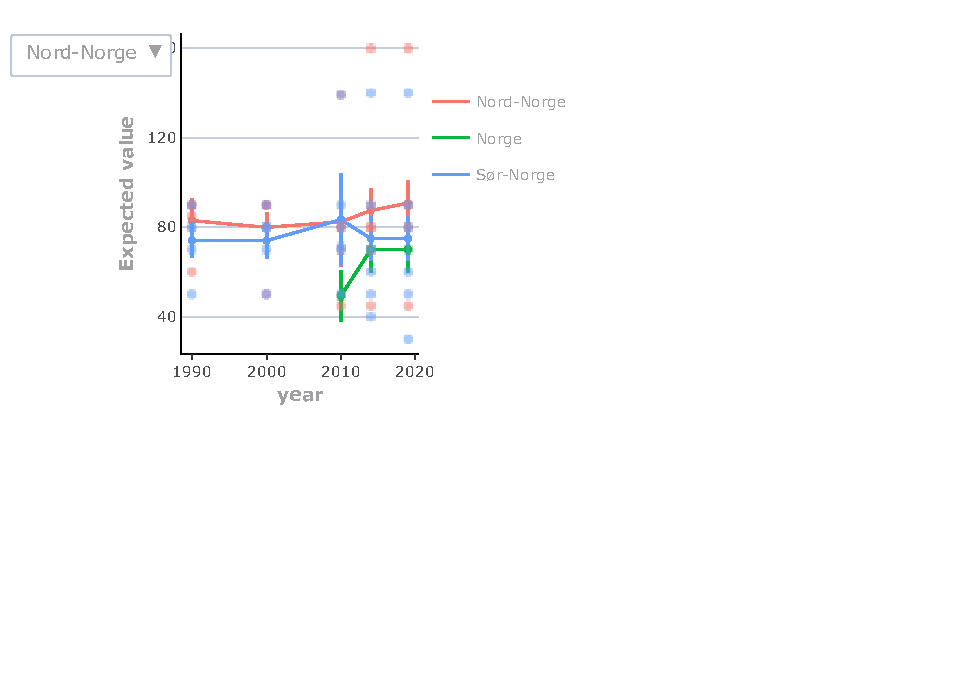
\includegraphics{02-time_series_files/figure-latex/raw data-1.pdf}

\hypertarget{scaled-data}{%
\section{Scaled data}\label{scaled-data}}

\begin{Shaded}
\begin{Highlighting}[]
\NormalTok{Elg\_assemebled}\OtherTok{\textless{}{-}} \FunctionTok{readRDS}\NormalTok{(}\StringTok{"data/Elg\_assemebled.rds"}\NormalTok{)}
\NormalTok{mycols}\OtherTok{=}\FunctionTok{c}\NormalTok{(}\StringTok{"ICunitName"}\NormalTok{ ,}\StringTok{"yearName"}\NormalTok{, }\StringTok{"expectedValue"}\NormalTok{,}\StringTok{"lowerQuantile"}\NormalTok{, }\StringTok{"upperQuantile"}\NormalTok{)}

\NormalTok{data\_list}\OtherTok{\textless{}{-}}\FunctionTok{lapply}\NormalTok{(Elg\_assemebled}\SpecialCharTok{$}\NormalTok{indicatorValues, }\ControlFlowTok{function}\NormalTok{(x) x}\SpecialCharTok{\%\textgreater{}\%} \FunctionTok{select}\NormalTok{(mycols))}

\NormalTok{dat}\OtherTok{\textless{}{-}}\FunctionTok{bind\_rows}\NormalTok{(data\_list, }\AttributeTok{.id =} \StringTok{"column\_label"}\NormalTok{)}

\CommentTok{\# plot}
\NormalTok{sum\_dat}\OtherTok{=}\NormalTok{dat }\SpecialCharTok{\%\textgreater{}\%} 
  \FunctionTok{group\_by}\NormalTok{(ICunitName, yearName) }\SpecialCharTok{\%\textgreater{}\%} 
  \FunctionTok{summarise}\NormalTok{(}\AttributeTok{mnExpected=}\FunctionTok{mean}\NormalTok{(expectedValue, }\AttributeTok{na.rm=}\ConstantTok{TRUE}\NormalTok{),}
            \AttributeTok{mnUpper=}\FunctionTok{mean}\NormalTok{(upperQuantile, }\AttributeTok{na.rm=}\ConstantTok{TRUE}\NormalTok{),}
            \AttributeTok{mnLower=}\FunctionTok{mean}\NormalTok{(lowerQuantile, }\AttributeTok{na.rm=}\ConstantTok{TRUE}\NormalTok{)) }\CommentTok{\# summerise the data to mean values}
\FunctionTok{source}\NormalTok{(}\StringTok{"R/ggplotTheme.R"}\NormalTok{)}
\NormalTok{p}\OtherTok{=}\NormalTok{sum\_dat }\SpecialCharTok{\%\textgreater{}\%} 
  \FunctionTok{ggplot}\NormalTok{(}\FunctionTok{aes}\NormalTok{(}\FunctionTok{as.numeric}\NormalTok{(yearName), mnExpected, }\AttributeTok{col=}\NormalTok{ICunitName))}\SpecialCharTok{+}
  \FunctionTok{geom\_line}\NormalTok{()}\SpecialCharTok{+}
  \FunctionTok{geom\_pointrange}\NormalTok{(}\FunctionTok{aes}\NormalTok{(}\AttributeTok{x=}\FunctionTok{as.numeric}\NormalTok{(yearName), }\AttributeTok{y=}\NormalTok{mnExpected, }\AttributeTok{ymin=}\NormalTok{mnLower, }\AttributeTok{ymax=}\NormalTok{mnUpper))}\SpecialCharTok{+}
  \FunctionTok{geom\_point}\NormalTok{(}\AttributeTok{data=}\NormalTok{dat, }\FunctionTok{aes}\NormalTok{(}\FunctionTok{as.numeric}\NormalTok{(yearName), expectedValue, }\AttributeTok{alpha=}\FloatTok{0.2}\NormalTok{))}\SpecialCharTok{+}
  \FunctionTok{labs}\NormalTok{(}\AttributeTok{x=}\StringTok{"year"}\NormalTok{, }\AttributeTok{y=}\StringTok{"Expected value"}\NormalTok{)}\SpecialCharTok{+}
  \FunctionTok{theme\_NIseries}\NormalTok{()}
\NormalTok{p2}\OtherTok{=}\FunctionTok{ggplotly}\NormalTok{(p)}
\NormalTok{p2 }\SpecialCharTok{\%\textgreater{}\%} \FunctionTok{layout}\NormalTok{(}
  \AttributeTok{updatemenus =} \FunctionTok{list}\NormalTok{(}
    \FunctionTok{list}\NormalTok{(}
      \AttributeTok{type =} \StringTok{"list"}\NormalTok{,}
      \AttributeTok{label =} \StringTok{\textquotesingle{}Category\textquotesingle{}}\NormalTok{,}
      \AttributeTok{buttons =} \FunctionTok{list}\NormalTok{(}
        \FunctionTok{list}\NormalTok{(}\AttributeTok{method =} \StringTok{"restyle"}\NormalTok{,}
             \AttributeTok{args =} \FunctionTok{list}\NormalTok{(}\StringTok{\textquotesingle{}visible\textquotesingle{}}\NormalTok{, }\FunctionTok{c}\NormalTok{(}\ConstantTok{TRUE}\NormalTok{, }\ConstantTok{FALSE}\NormalTok{, }\ConstantTok{FALSE}\NormalTok{, }\ConstantTok{FALSE}\NormalTok{, }\ConstantTok{FALSE}\NormalTok{, }\ConstantTok{FALSE}\NormalTok{, }\ConstantTok{FALSE}\NormalTok{, }\ConstantTok{FALSE}\NormalTok{, }\ConstantTok{FALSE}\NormalTok{, }\ConstantTok{FALSE}\NormalTok{, }\ConstantTok{FALSE}\NormalTok{, }\ConstantTok{FALSE}\NormalTok{, }\ConstantTok{FALSE}\NormalTok{, }\ConstantTok{FALSE}\NormalTok{, }\ConstantTok{FALSE}\NormalTok{, }\ConstantTok{FALSE}\NormalTok{, }\ConstantTok{FALSE}\NormalTok{, }\ConstantTok{FALSE}\NormalTok{)),}
             \AttributeTok{label =} \FunctionTok{unique}\NormalTok{(dat}\SpecialCharTok{$}\NormalTok{ICunitName)[}\DecValTok{2}\NormalTok{]),}
        \FunctionTok{list}\NormalTok{(}\AttributeTok{method =} \StringTok{"restyle"}\NormalTok{,}
             \AttributeTok{args =} \FunctionTok{list}\NormalTok{(}\StringTok{\textquotesingle{}visible\textquotesingle{}}\NormalTok{, }\FunctionTok{c}\NormalTok{(}\ConstantTok{FALSE}\NormalTok{, }\ConstantTok{TRUE}\NormalTok{, }\ConstantTok{FALSE}\NormalTok{, }\ConstantTok{FALSE}\NormalTok{, }\ConstantTok{FALSE}\NormalTok{, }\ConstantTok{FALSE}\NormalTok{, }\ConstantTok{FALSE}\NormalTok{, }\ConstantTok{FALSE}\NormalTok{, }\ConstantTok{FALSE}\NormalTok{, }\ConstantTok{FALSE}\NormalTok{, }\ConstantTok{FALSE}\NormalTok{, }\ConstantTok{FALSE}\NormalTok{, }\ConstantTok{FALSE}\NormalTok{, }\ConstantTok{FALSE}\NormalTok{, }\ConstantTok{FALSE}\NormalTok{, }\ConstantTok{FALSE}\NormalTok{, }\ConstantTok{FALSE}\NormalTok{, }\ConstantTok{FALSE}\NormalTok{)),}
             \AttributeTok{label =} \FunctionTok{unique}\NormalTok{(dat}\SpecialCharTok{$}\NormalTok{ICunitName)[}\DecValTok{8}\NormalTok{]),}
        \FunctionTok{list}\NormalTok{(}\AttributeTok{method =} \StringTok{"restyle"}\NormalTok{,}
             \AttributeTok{args =} \FunctionTok{list}\NormalTok{(}\StringTok{\textquotesingle{}visible\textquotesingle{}}\NormalTok{, }\FunctionTok{c}\NormalTok{(}\ConstantTok{FALSE}\NormalTok{, }\ConstantTok{FALSE}\NormalTok{,}\ConstantTok{TRUE}\NormalTok{, }\ConstantTok{FALSE}\NormalTok{, }\ConstantTok{FALSE}\NormalTok{, }\ConstantTok{FALSE}\NormalTok{, }\ConstantTok{FALSE}\NormalTok{, }\ConstantTok{FALSE}\NormalTok{, }\ConstantTok{FALSE}\NormalTok{, }\ConstantTok{FALSE}\NormalTok{, }\ConstantTok{FALSE}\NormalTok{, }\ConstantTok{FALSE}\NormalTok{, }\ConstantTok{FALSE}\NormalTok{, }\ConstantTok{FALSE}\NormalTok{, }\ConstantTok{FALSE}\NormalTok{, }\ConstantTok{FALSE}\NormalTok{, }\ConstantTok{FALSE}\NormalTok{, }\ConstantTok{FALSE}\NormalTok{)),}
             \AttributeTok{label =} \FunctionTok{unique}\NormalTok{(dat}\SpecialCharTok{$}\NormalTok{ICunitName)[}\DecValTok{5}\NormalTok{]),}
        \FunctionTok{list}\NormalTok{(}\AttributeTok{method =} \StringTok{"restyle"}\NormalTok{,}
             \AttributeTok{args =} \FunctionTok{list}\NormalTok{(}\StringTok{\textquotesingle{}visible\textquotesingle{}}\NormalTok{, }\FunctionTok{c}\NormalTok{( }\ConstantTok{FALSE}\NormalTok{, }\ConstantTok{FALSE}\NormalTok{, }\ConstantTok{FALSE}\NormalTok{,}\ConstantTok{TRUE}\NormalTok{, }\ConstantTok{FALSE}\NormalTok{, }\ConstantTok{FALSE}\NormalTok{, }\ConstantTok{FALSE}\NormalTok{, }\ConstantTok{FALSE}\NormalTok{, }\ConstantTok{FALSE}\NormalTok{, }\ConstantTok{FALSE}\NormalTok{, }\ConstantTok{FALSE}\NormalTok{, }\ConstantTok{FALSE}\NormalTok{, }\ConstantTok{FALSE}\NormalTok{, }\ConstantTok{FALSE}\NormalTok{, }\ConstantTok{FALSE}\NormalTok{, }\ConstantTok{FALSE}\NormalTok{, }\ConstantTok{FALSE}\NormalTok{, }\ConstantTok{FALSE}\NormalTok{)),}
             \AttributeTok{label =} \FunctionTok{unique}\NormalTok{(dat}\SpecialCharTok{$}\NormalTok{ICunitName)[}\DecValTok{18}\NormalTok{]),}
        \FunctionTok{list}\NormalTok{(}\AttributeTok{method =} \StringTok{"restyle"}\NormalTok{,}
             \AttributeTok{args =} \FunctionTok{list}\NormalTok{(}\StringTok{\textquotesingle{}visible\textquotesingle{}}\NormalTok{, }\FunctionTok{c}\NormalTok{(}\ConstantTok{FALSE}\NormalTok{, }\ConstantTok{FALSE}\NormalTok{, }\ConstantTok{FALSE}\NormalTok{,}\ConstantTok{FALSE}\NormalTok{, }\ConstantTok{TRUE}\NormalTok{, }\ConstantTok{FALSE}\NormalTok{, }\ConstantTok{FALSE}\NormalTok{, }\ConstantTok{FALSE}\NormalTok{, }\ConstantTok{FALSE}\NormalTok{, }\ConstantTok{FALSE}\NormalTok{, }\ConstantTok{FALSE}\NormalTok{, }\ConstantTok{FALSE}\NormalTok{, }\ConstantTok{FALSE}\NormalTok{, }\ConstantTok{FALSE}\NormalTok{, }\ConstantTok{FALSE}\NormalTok{, }\ConstantTok{FALSE}\NormalTok{, }\ConstantTok{FALSE}\NormalTok{, }\ConstantTok{FALSE}\NormalTok{)),}
             \AttributeTok{label =} \FunctionTok{unique}\NormalTok{(dat}\SpecialCharTok{$}\NormalTok{ICunitName)[}\DecValTok{3}\NormalTok{]),}
        \FunctionTok{list}\NormalTok{(}\AttributeTok{method =} \StringTok{"restyle"}\NormalTok{,}
             \AttributeTok{args =} \FunctionTok{list}\NormalTok{(}\StringTok{\textquotesingle{}visible\textquotesingle{}}\NormalTok{, }\FunctionTok{c}\NormalTok{( }\ConstantTok{FALSE}\NormalTok{, }\ConstantTok{FALSE}\NormalTok{, }\ConstantTok{FALSE}\NormalTok{,}\ConstantTok{FALSE}\NormalTok{, }\ConstantTok{FALSE}\NormalTok{, }\ConstantTok{TRUE}\NormalTok{, }\ConstantTok{FALSE}\NormalTok{, }\ConstantTok{FALSE}\NormalTok{, }\ConstantTok{FALSE}\NormalTok{, }\ConstantTok{FALSE}\NormalTok{, }\ConstantTok{FALSE}\NormalTok{, }\ConstantTok{FALSE}\NormalTok{, }\ConstantTok{FALSE}\NormalTok{, }\ConstantTok{FALSE}\NormalTok{, }\ConstantTok{FALSE}\NormalTok{, }\ConstantTok{FALSE}\NormalTok{, }\ConstantTok{FALSE}\NormalTok{, }\ConstantTok{FALSE}\NormalTok{)),}
             \AttributeTok{label =} \FunctionTok{unique}\NormalTok{(dat}\SpecialCharTok{$}\NormalTok{ICunitName)[}\DecValTok{11}\NormalTok{]),}
        \FunctionTok{list}\NormalTok{(}\AttributeTok{method =} \StringTok{"restyle"}\NormalTok{,}
             \AttributeTok{args =} \FunctionTok{list}\NormalTok{(}\StringTok{\textquotesingle{}visible\textquotesingle{}}\NormalTok{, }\FunctionTok{c}\NormalTok{( }\ConstantTok{FALSE}\NormalTok{, }\ConstantTok{FALSE}\NormalTok{, }\ConstantTok{FALSE}\NormalTok{,}\ConstantTok{FALSE}\NormalTok{, }\ConstantTok{FALSE}\NormalTok{, }\ConstantTok{FALSE}\NormalTok{, }\ConstantTok{TRUE}\NormalTok{, }\ConstantTok{FALSE}\NormalTok{, }\ConstantTok{FALSE}\NormalTok{, }\ConstantTok{FALSE}\NormalTok{, }\ConstantTok{FALSE}\NormalTok{, }\ConstantTok{FALSE}\NormalTok{, }\ConstantTok{FALSE}\NormalTok{, }\ConstantTok{FALSE}\NormalTok{, }\ConstantTok{FALSE}\NormalTok{, }\ConstantTok{FALSE}\NormalTok{, }\ConstantTok{FALSE}\NormalTok{, }\ConstantTok{FALSE}\NormalTok{)),}
             \AttributeTok{label =} \FunctionTok{unique}\NormalTok{(dat}\SpecialCharTok{$}\NormalTok{ICunitName)[}\DecValTok{13}\NormalTok{]),}
        \FunctionTok{list}\NormalTok{(}\AttributeTok{method =} \StringTok{"restyle"}\NormalTok{,}
             \AttributeTok{args =} \FunctionTok{list}\NormalTok{(}\StringTok{\textquotesingle{}visible\textquotesingle{}}\NormalTok{, }\FunctionTok{c}\NormalTok{( }\ConstantTok{FALSE}\NormalTok{, }\ConstantTok{FALSE}\NormalTok{, }\ConstantTok{FALSE}\NormalTok{,}\ConstantTok{FALSE}\NormalTok{, }\ConstantTok{FALSE}\NormalTok{, }\ConstantTok{FALSE}\NormalTok{, }\ConstantTok{FALSE}\NormalTok{, }\ConstantTok{TRUE}\NormalTok{, }\ConstantTok{FALSE}\NormalTok{, }\ConstantTok{FALSE}\NormalTok{, }\ConstantTok{FALSE}\NormalTok{, }\ConstantTok{FALSE}\NormalTok{, }\ConstantTok{FALSE}\NormalTok{, }\ConstantTok{FALSE}\NormalTok{, }\ConstantTok{FALSE}\NormalTok{, }\ConstantTok{FALSE}\NormalTok{, }\ConstantTok{FALSE}\NormalTok{, }\ConstantTok{FALSE}\NormalTok{)),}
             \AttributeTok{label =} \FunctionTok{unique}\NormalTok{(dat}\SpecialCharTok{$}\NormalTok{ICunitName)[}\DecValTok{15}\NormalTok{]),}
        \FunctionTok{list}\NormalTok{(}\AttributeTok{method =} \StringTok{"restyle"}\NormalTok{,}
             \AttributeTok{args =} \FunctionTok{list}\NormalTok{(}\StringTok{\textquotesingle{}visible\textquotesingle{}}\NormalTok{, }\FunctionTok{c}\NormalTok{( }\ConstantTok{FALSE}\NormalTok{, }\ConstantTok{FALSE}\NormalTok{, }\ConstantTok{FALSE}\NormalTok{,}\ConstantTok{FALSE}\NormalTok{, }\ConstantTok{FALSE}\NormalTok{, }\ConstantTok{FALSE}\NormalTok{, }\ConstantTok{FALSE}\NormalTok{, }\ConstantTok{FALSE}\NormalTok{, }\ConstantTok{TRUE}\NormalTok{, }\ConstantTok{FALSE}\NormalTok{, }\ConstantTok{FALSE}\NormalTok{, }\ConstantTok{FALSE}\NormalTok{, }\ConstantTok{FALSE}\NormalTok{, }\ConstantTok{FALSE}\NormalTok{, }\ConstantTok{FALSE}\NormalTok{, }\ConstantTok{FALSE}\NormalTok{, }\ConstantTok{FALSE}\NormalTok{, }\ConstantTok{FALSE}\NormalTok{)),}
             \AttributeTok{label =} \FunctionTok{unique}\NormalTok{(dat}\SpecialCharTok{$}\NormalTok{ICunitName)[}\DecValTok{16}\NormalTok{]),}
        \FunctionTok{list}\NormalTok{(}\AttributeTok{method =} \StringTok{"restyle"}\NormalTok{,}
             \AttributeTok{args =} \FunctionTok{list}\NormalTok{(}\StringTok{\textquotesingle{}visible\textquotesingle{}}\NormalTok{, }\FunctionTok{c}\NormalTok{( }\ConstantTok{FALSE}\NormalTok{, }\ConstantTok{FALSE}\NormalTok{, }\ConstantTok{FALSE}\NormalTok{,}\ConstantTok{FALSE}\NormalTok{, }\ConstantTok{FALSE}\NormalTok{, }\ConstantTok{FALSE}\NormalTok{, }\ConstantTok{FALSE}\NormalTok{, }\ConstantTok{FALSE}\NormalTok{, }\ConstantTok{FALSE}\NormalTok{, }\ConstantTok{TRUE}\NormalTok{, }\ConstantTok{FALSE}\NormalTok{, }\ConstantTok{FALSE}\NormalTok{, }\ConstantTok{FALSE}\NormalTok{, }\ConstantTok{FALSE}\NormalTok{, }\ConstantTok{FALSE}\NormalTok{, }\ConstantTok{FALSE}\NormalTok{, }\ConstantTok{FALSE}\NormalTok{, }\ConstantTok{FALSE}\NormalTok{)),}
             \AttributeTok{label =} \FunctionTok{unique}\NormalTok{(dat}\SpecialCharTok{$}\NormalTok{ICunitName)[}\DecValTok{4}\NormalTok{]),}
        \FunctionTok{list}\NormalTok{(}\AttributeTok{method =} \StringTok{"restyle"}\NormalTok{,}
             \AttributeTok{args =} \FunctionTok{list}\NormalTok{(}\StringTok{\textquotesingle{}visible\textquotesingle{}}\NormalTok{, }\FunctionTok{c}\NormalTok{( }\ConstantTok{FALSE}\NormalTok{, }\ConstantTok{FALSE}\NormalTok{, }\ConstantTok{FALSE}\NormalTok{,}\ConstantTok{FALSE}\NormalTok{, }\ConstantTok{FALSE}\NormalTok{, }\ConstantTok{FALSE}\NormalTok{, }\ConstantTok{FALSE}\NormalTok{, }\ConstantTok{FALSE}\NormalTok{, }\ConstantTok{FALSE}\NormalTok{, }\ConstantTok{FALSE}\NormalTok{, }\ConstantTok{TRUE}\NormalTok{, }\ConstantTok{FALSE}\NormalTok{, }\ConstantTok{FALSE}\NormalTok{, }\ConstantTok{FALSE}\NormalTok{, }\ConstantTok{FALSE}\NormalTok{, }\ConstantTok{FALSE}\NormalTok{, }\ConstantTok{FALSE}\NormalTok{, }\ConstantTok{FALSE}\NormalTok{)),}
             \AttributeTok{label =} \FunctionTok{unique}\NormalTok{(dat}\SpecialCharTok{$}\NormalTok{ICunitName)[}\DecValTok{10}\NormalTok{]),}
        \FunctionTok{list}\NormalTok{(}\AttributeTok{method =} \StringTok{"restyle"}\NormalTok{,}
             \AttributeTok{args =} \FunctionTok{list}\NormalTok{(}\StringTok{\textquotesingle{}visible\textquotesingle{}}\NormalTok{, }\FunctionTok{c}\NormalTok{( }\ConstantTok{FALSE}\NormalTok{, }\ConstantTok{FALSE}\NormalTok{, }\ConstantTok{FALSE}\NormalTok{,}\ConstantTok{FALSE}\NormalTok{, }\ConstantTok{FALSE}\NormalTok{, }\ConstantTok{FALSE}\NormalTok{, }\ConstantTok{FALSE}\NormalTok{, }\ConstantTok{FALSE}\NormalTok{, }\ConstantTok{FALSE}\NormalTok{, }\ConstantTok{FALSE}\NormalTok{, }\ConstantTok{FALSE}\NormalTok{, }\ConstantTok{TRUE}\NormalTok{, }\ConstantTok{FALSE}\NormalTok{, }\ConstantTok{FALSE}\NormalTok{, }\ConstantTok{FALSE}\NormalTok{, }\ConstantTok{FALSE}\NormalTok{, }\ConstantTok{FALSE}\NormalTok{, }\ConstantTok{FALSE}\NormalTok{)),}
             \AttributeTok{label =} \FunctionTok{unique}\NormalTok{(dat}\SpecialCharTok{$}\NormalTok{ICunitName)[}\DecValTok{12}\NormalTok{]),}
        \FunctionTok{list}\NormalTok{(}\AttributeTok{method =} \StringTok{"restyle"}\NormalTok{,}
             \AttributeTok{args =} \FunctionTok{list}\NormalTok{(}\StringTok{\textquotesingle{}visible\textquotesingle{}}\NormalTok{, }\FunctionTok{c}\NormalTok{( }\ConstantTok{FALSE}\NormalTok{, }\ConstantTok{FALSE}\NormalTok{, }\ConstantTok{FALSE}\NormalTok{,}\ConstantTok{FALSE}\NormalTok{, }\ConstantTok{FALSE}\NormalTok{, }\ConstantTok{FALSE}\NormalTok{, }\ConstantTok{FALSE}\NormalTok{, }\ConstantTok{FALSE}\NormalTok{, }\ConstantTok{FALSE}\NormalTok{, }\ConstantTok{FALSE}\NormalTok{, }\ConstantTok{FALSE}\NormalTok{, }\ConstantTok{FALSE}\NormalTok{, }\ConstantTok{TRUE}\NormalTok{, }\ConstantTok{FALSE}\NormalTok{, }\ConstantTok{FALSE}\NormalTok{, }\ConstantTok{FALSE}\NormalTok{, }\ConstantTok{FALSE}\NormalTok{, }\ConstantTok{FALSE}\NormalTok{)),}
             \AttributeTok{label =} \FunctionTok{unique}\NormalTok{(dat}\SpecialCharTok{$}\NormalTok{ICunitName)[}\DecValTok{14}\NormalTok{]),}
        \FunctionTok{list}\NormalTok{(}\AttributeTok{method =} \StringTok{"restyle"}\NormalTok{,}
             \AttributeTok{args =} \FunctionTok{list}\NormalTok{(}\StringTok{\textquotesingle{}visible\textquotesingle{}}\NormalTok{, }\FunctionTok{c}\NormalTok{( }\ConstantTok{FALSE}\NormalTok{, }\ConstantTok{FALSE}\NormalTok{, }\ConstantTok{FALSE}\NormalTok{,}\ConstantTok{FALSE}\NormalTok{, }\ConstantTok{FALSE}\NormalTok{, }\ConstantTok{FALSE}\NormalTok{, }\ConstantTok{FALSE}\NormalTok{, }\ConstantTok{FALSE}\NormalTok{, }\ConstantTok{FALSE}\NormalTok{, }\ConstantTok{FALSE}\NormalTok{, }\ConstantTok{FALSE}\NormalTok{, }\ConstantTok{FALSE}\NormalTok{, }\ConstantTok{FALSE}\NormalTok{, }\ConstantTok{TRUE}\NormalTok{, }\ConstantTok{FALSE}\NormalTok{, }\ConstantTok{FALSE}\NormalTok{, }\ConstantTok{FALSE}\NormalTok{, }\ConstantTok{FALSE}\NormalTok{)),}
             \AttributeTok{label =} \FunctionTok{unique}\NormalTok{(dat}\SpecialCharTok{$}\NormalTok{ICunitName)[}\DecValTok{7}\NormalTok{]),}
        \FunctionTok{list}\NormalTok{(}\AttributeTok{method =} \StringTok{"restyle"}\NormalTok{,}
             \AttributeTok{args =} \FunctionTok{list}\NormalTok{(}\StringTok{\textquotesingle{}visible\textquotesingle{}}\NormalTok{, }\FunctionTok{c}\NormalTok{( }\ConstantTok{FALSE}\NormalTok{, }\ConstantTok{FALSE}\NormalTok{, }\ConstantTok{FALSE}\NormalTok{,}\ConstantTok{FALSE}\NormalTok{, }\ConstantTok{FALSE}\NormalTok{, }\ConstantTok{FALSE}\NormalTok{, }\ConstantTok{FALSE}\NormalTok{, }\ConstantTok{FALSE}\NormalTok{, }\ConstantTok{FALSE}\NormalTok{, }\ConstantTok{FALSE}\NormalTok{, }\ConstantTok{FALSE}\NormalTok{, }\ConstantTok{FALSE}\NormalTok{, }\ConstantTok{FALSE}\NormalTok{, }\ConstantTok{FALSE}\NormalTok{, }\ConstantTok{TRUE}\NormalTok{, }\ConstantTok{FALSE}\NormalTok{, }\ConstantTok{FALSE}\NormalTok{, }\ConstantTok{FALSE}\NormalTok{)),}
             \AttributeTok{label =} \FunctionTok{unique}\NormalTok{(dat}\SpecialCharTok{$}\NormalTok{ICunitName)[}\DecValTok{17}\NormalTok{]),}
        \FunctionTok{list}\NormalTok{(}\AttributeTok{method =} \StringTok{"restyle"}\NormalTok{,}
             \AttributeTok{args =} \FunctionTok{list}\NormalTok{(}\StringTok{\textquotesingle{}visible\textquotesingle{}}\NormalTok{, }\FunctionTok{c}\NormalTok{( }\ConstantTok{FALSE}\NormalTok{, }\ConstantTok{FALSE}\NormalTok{, }\ConstantTok{FALSE}\NormalTok{,}\ConstantTok{FALSE}\NormalTok{, }\ConstantTok{FALSE}\NormalTok{, }\ConstantTok{FALSE}\NormalTok{, }\ConstantTok{FALSE}\NormalTok{, }\ConstantTok{FALSE}\NormalTok{, }\ConstantTok{FALSE}\NormalTok{, }\ConstantTok{FALSE}\NormalTok{, }\ConstantTok{FALSE}\NormalTok{, }\ConstantTok{FALSE}\NormalTok{, }\ConstantTok{FALSE}\NormalTok{, }\ConstantTok{FALSE}\NormalTok{, }\ConstantTok{FALSE}\NormalTok{, }\ConstantTok{TRUE}\NormalTok{, }\ConstantTok{FALSE}\NormalTok{, }\ConstantTok{FALSE}\NormalTok{)),}
             \AttributeTok{label =} \FunctionTok{unique}\NormalTok{(dat}\SpecialCharTok{$}\NormalTok{ICunitName)[}\DecValTok{9}\NormalTok{]),}
        \FunctionTok{list}\NormalTok{(}\AttributeTok{method =} \StringTok{"restyle"}\NormalTok{,}
             \AttributeTok{args =} \FunctionTok{list}\NormalTok{(}\StringTok{\textquotesingle{}visible\textquotesingle{}}\NormalTok{, }\FunctionTok{c}\NormalTok{( }\ConstantTok{FALSE}\NormalTok{, }\ConstantTok{FALSE}\NormalTok{, }\ConstantTok{FALSE}\NormalTok{,}\ConstantTok{FALSE}\NormalTok{, }\ConstantTok{FALSE}\NormalTok{, }\ConstantTok{FALSE}\NormalTok{, }\ConstantTok{FALSE}\NormalTok{, }\ConstantTok{FALSE}\NormalTok{, }\ConstantTok{FALSE}\NormalTok{, }\ConstantTok{FALSE}\NormalTok{, }\ConstantTok{FALSE}\NormalTok{, }\ConstantTok{FALSE}\NormalTok{, }\ConstantTok{FALSE}\NormalTok{, }\ConstantTok{FALSE}\NormalTok{, }\ConstantTok{FALSE}\NormalTok{, }\ConstantTok{FALSE}\NormalTok{, }\ConstantTok{TRUE}\NormalTok{, }\ConstantTok{FALSE}\NormalTok{)),}
             \AttributeTok{label =} \FunctionTok{unique}\NormalTok{(dat}\SpecialCharTok{$}\NormalTok{ICunitName)[}\DecValTok{6}\NormalTok{]),}
        \FunctionTok{list}\NormalTok{(}\AttributeTok{method =} \StringTok{"restyle"}\NormalTok{,}
             \AttributeTok{args =} \FunctionTok{list}\NormalTok{(}\StringTok{\textquotesingle{}visible\textquotesingle{}}\NormalTok{, }\FunctionTok{c}\NormalTok{( }\ConstantTok{FALSE}\NormalTok{, }\ConstantTok{FALSE}\NormalTok{, }\ConstantTok{FALSE}\NormalTok{,}\ConstantTok{FALSE}\NormalTok{, }\ConstantTok{FALSE}\NormalTok{, }\ConstantTok{FALSE}\NormalTok{, }\ConstantTok{FALSE}\NormalTok{, }\ConstantTok{FALSE}\NormalTok{, }\ConstantTok{FALSE}\NormalTok{, }\ConstantTok{FALSE}\NormalTok{, }\ConstantTok{FALSE}\NormalTok{, }\ConstantTok{FALSE}\NormalTok{, }\ConstantTok{FALSE}\NormalTok{, }\ConstantTok{FALSE}\NormalTok{, }\ConstantTok{FALSE}\NormalTok{, }\ConstantTok{FALSE}\NormalTok{, }\ConstantTok{FALSE}\NormalTok{, }\ConstantTok{TRUE}\NormalTok{)),}
             \AttributeTok{label =} \FunctionTok{unique}\NormalTok{(dat}\SpecialCharTok{$}\NormalTok{ICunitName)[}\DecValTok{1}\NormalTok{])}
\NormalTok{      )}
\NormalTok{    )}
\NormalTok{  )}
\NormalTok{) }\CommentTok{\# Add drop down menus for the data}
\end{Highlighting}
\end{Shaded}

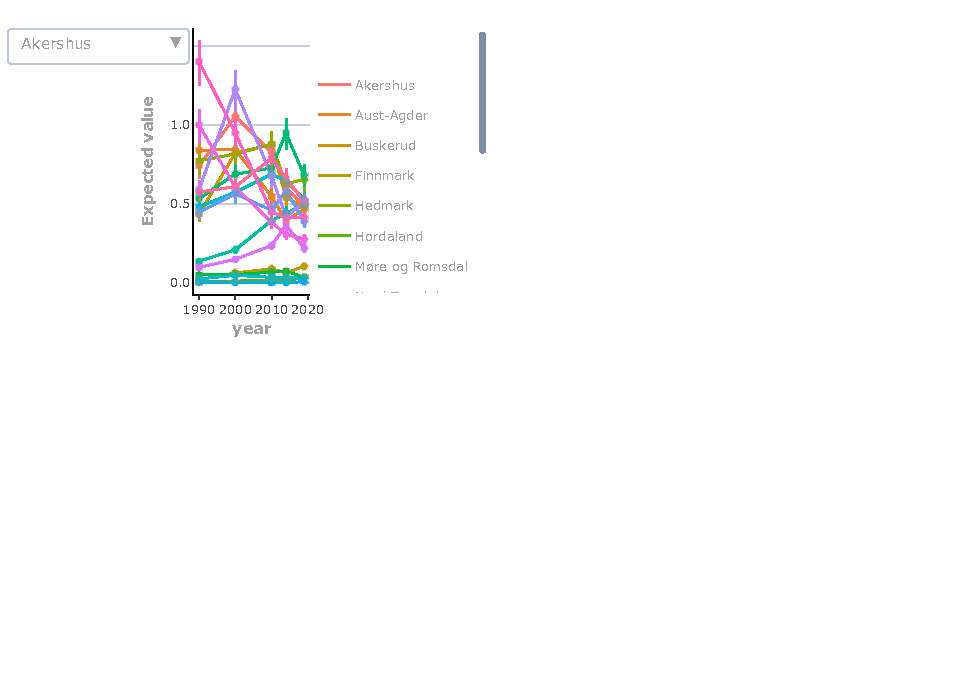
\includegraphics{02-time_series_files/figure-latex/scaled data-1.pdf}

\hypertarget{maps}{%
\chapter{Maps}\label{maps}}

\hypertarget{raw-data-1}{%
\section{Raw data}\label{raw-data-1}}

\hypertarget{scaled-data-1}{%
\section{Scaled data}\label{scaled-data-1}}

\hypertarget{jerv}{%
\subsection{Jerv}\label{jerv}}

\hypertarget{prepare-ni-data}{%
\subsubsection{Prepare NI data}\label{prepare-ni-data}}

The jerv (wolverine) data was downloaded using the \texttt{R/singleIndicator.R} script and the importDatasetApi() function,, and subsequently the assembleNiObject() function, so now I can simply import it.

\begin{Shaded}
\begin{Highlighting}[]
\NormalTok{jerv }\OtherTok{\textless{}{-}} \FunctionTok{readRDS}\NormalTok{(}\StringTok{"data/Jerv\_assemebled.rds"}\NormalTok{)}
\end{Highlighting}
\end{Shaded}

This data file contains the raw data in the form of expected values for each BSunits (municipalities). But we actually want to keep the original geometeris of the eight rovviltregioner, and so we need to focus in the ICunits instead.

\begin{Shaded}
\begin{Highlighting}[]
\FunctionTok{par}\NormalTok{(}\AttributeTok{mar=}\FunctionTok{c}\NormalTok{(}\DecValTok{9}\NormalTok{,}\DecValTok{5}\NormalTok{,}\DecValTok{1}\NormalTok{,}\DecValTok{1}\NormalTok{))}
\FunctionTok{barplot}\NormalTok{(jerv}\SpecialCharTok{$}\NormalTok{indicatorValues}\SpecialCharTok{$}\StringTok{\textasciigrave{}}\AttributeTok{2019}\StringTok{\textasciigrave{}}\SpecialCharTok{$}\NormalTok{expectedValue,}
        \AttributeTok{names.arg =}\NormalTok{ jerv}\SpecialCharTok{$}\NormalTok{indicatorValues}\SpecialCharTok{$}\StringTok{\textasciigrave{}}\AttributeTok{2019}\StringTok{\textasciigrave{}}\SpecialCharTok{$}\NormalTok{ICunitName, }
        \AttributeTok{las=}\DecValTok{2}\NormalTok{,}
        \AttributeTok{ylab =} \StringTok{"Estimated number of}\SpecialCharTok{\textbackslash{}n}\StringTok{wolverine in 2019"}\NormalTok{)}
\end{Highlighting}
\end{Shaded}

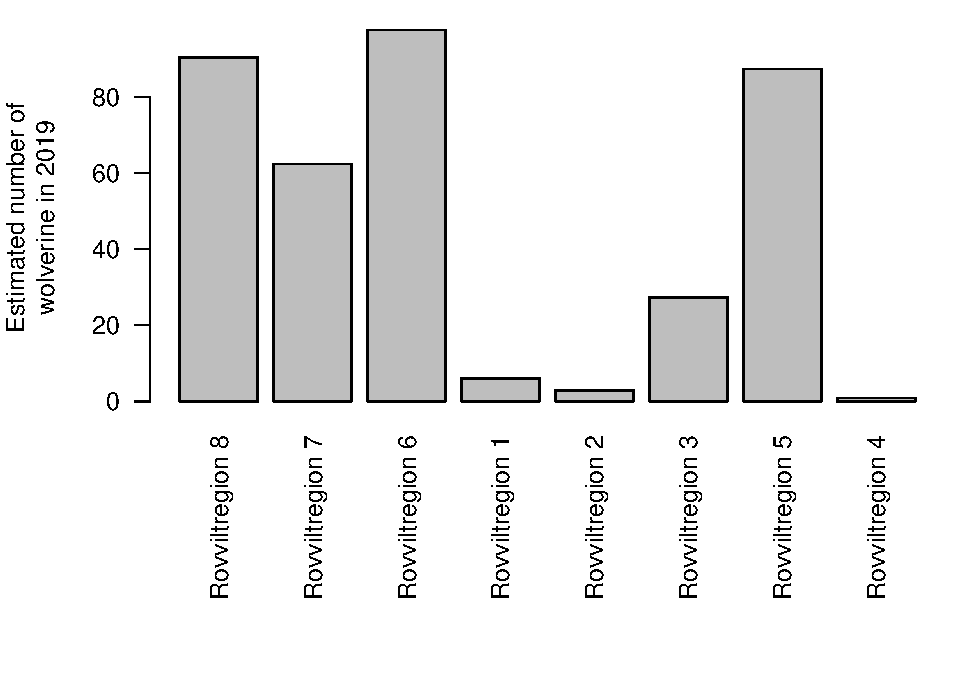
\includegraphics{03-maps_files/figure-latex/unnamed-chunk-3-1.pdf}

The data also contains upper and lower quantiles, but we can also get the full probability distribution and sample from it to get standard deviations.
but also as probability functions that we can sample from:

\begin{Shaded}
\begin{Highlighting}[]
\CommentTok{\# bruker tradOb siden custumDist er NA. Dette er ikke en generisk løsning. }
\NormalTok{obstype }\OtherTok{\textless{}{-}} \FunctionTok{rep}\NormalTok{(}\StringTok{"tradObs"}\NormalTok{, }\FunctionTok{nrow}\NormalTok{(jerv}\SpecialCharTok{$}\NormalTok{indicatorValues}\SpecialCharTok{$}\StringTok{\textquotesingle{}2019\textquotesingle{}}\NormalTok{))}

\CommentTok{\#myYears \textless{}{-} as.character(c(1990,2000,2010,2014,2019))}
\NormalTok{myYears }\OtherTok{\textless{}{-}} \FunctionTok{as.character}\NormalTok{(}\FunctionTok{c}\NormalTok{(}\DecValTok{2019}\NormalTok{))}

\ControlFlowTok{for}\NormalTok{(i }\ControlFlowTok{in} \DecValTok{1}\SpecialCharTok{:}\FunctionTok{length}\NormalTok{(myYears))\{}
\CommentTok{\# print(i)}

\NormalTok{myMat }\OtherTok{\textless{}{-}}\NormalTok{ NIcalc}\SpecialCharTok{::}\FunctionTok{sampleObsMat}\NormalTok{(}
  \AttributeTok{ICunitId           =}\NormalTok{ jerv}\SpecialCharTok{$}\NormalTok{indicatorValues[[i]]}\SpecialCharTok{$}\NormalTok{ICunitId, }
  \AttributeTok{value              =}\NormalTok{ jerv}\SpecialCharTok{$}\NormalTok{indicatorValues[[i]]}\SpecialCharTok{$}\NormalTok{expectedValue,}
  \AttributeTok{distrib            =}\NormalTok{ jerv}\SpecialCharTok{$}\NormalTok{indicatorValues[[i]]}\SpecialCharTok{$}\NormalTok{distributionFamilyName,}
  \AttributeTok{mu                 =}\NormalTok{ jerv}\SpecialCharTok{$}\NormalTok{indicatorValues[[i]]}\SpecialCharTok{$}\NormalTok{distParameter1,}
  \AttributeTok{sig                =}\NormalTok{ jerv}\SpecialCharTok{$}\NormalTok{indicatorValues[[i]]}\SpecialCharTok{$}\NormalTok{distParameter2,}
  \AttributeTok{customDistribution =}\NormalTok{ jerv}\SpecialCharTok{$}\NormalTok{indicatorValues[[i]]}\SpecialCharTok{$}\NormalTok{customDistribution,}
          \AttributeTok{obsType =}\NormalTok{ obstype,}
          \AttributeTok{nsim =} \DecValTok{1000}
          
\NormalTok{)}
\FunctionTok{assign}\NormalTok{(}\FunctionTok{paste0}\NormalTok{(}\StringTok{"myMat"}\NormalTok{, myYears[i]), myMat)}
\NormalTok{\}}
\CommentTok{\#\textgreater{} Warning: replacing previous import \textquotesingle{}distr::plot\textquotesingle{} by}
\CommentTok{\#\textgreater{} \textquotesingle{}graphics::plot\textquotesingle{} when loading \textquotesingle{}NIcalc\textquotesingle{}}

\FunctionTok{par}\NormalTok{(}\AttributeTok{mfrow =} \FunctionTok{c}\NormalTok{(}\DecValTok{1}\NormalTok{,}\DecValTok{2}\NormalTok{))}
\FunctionTok{hist}\NormalTok{(myMat2019[}\DecValTok{1}\NormalTok{,], }\AttributeTok{main =} \StringTok{"Rovviltregion 1"}\NormalTok{, }\AttributeTok{xlab =} \StringTok{""}\NormalTok{)}
\FunctionTok{hist}\NormalTok{(myMat2019[}\DecValTok{8}\NormalTok{,], }\AttributeTok{main =} \StringTok{"Rovviltregion 8"}\NormalTok{, }\AttributeTok{xlab =} \StringTok{""}\NormalTok{)}
\end{Highlighting}
\end{Shaded}

\includegraphics{03-maps_files/figure-latex/unnamed-chunk-4-1.pdf}

For some reason the extected values are far from the mean of these distributions. I did this exercise \href{https://ninanor.github.io/IBECA/jerv.html}{once before}, and did not get this problem then. I think the difference is that I use eco = NULL this time, in the \texttt{importDatasetApi()}, and this cause the output to somehow split into forest and alpine ecosystems. I will ignore this here for this example.

I can also get the reference values in the same way, and then divide one by the other to get scaled values

\begin{Shaded}
\begin{Highlighting}[]
\NormalTok{myMatr }\OtherTok{\textless{}{-}}\NormalTok{ NIcalc}\SpecialCharTok{::}\FunctionTok{sampleObsMat}\NormalTok{(}
\NormalTok{            jerv}\SpecialCharTok{$}\NormalTok{referenceValues}\SpecialCharTok{$}\NormalTok{ICunitId, }
\NormalTok{            jerv}\SpecialCharTok{$}\NormalTok{referenceValues}\SpecialCharTok{$}\NormalTok{expectedValue,}
\NormalTok{            jerv}\SpecialCharTok{$}\NormalTok{referenceValues}\SpecialCharTok{$}\NormalTok{distributionFamilyName,}
            \AttributeTok{mu =}\NormalTok{ jerv}\SpecialCharTok{$}\NormalTok{referenceValues}\SpecialCharTok{$}\NormalTok{distParameter1,}
            \AttributeTok{sig =}\NormalTok{ jerv}\SpecialCharTok{$}\NormalTok{referenceValues}\SpecialCharTok{$}\NormalTok{distParameter2,}
            \AttributeTok{customDistribution =}\NormalTok{ jerv}\SpecialCharTok{$}\NormalTok{referenceValues}\SpecialCharTok{$}\NormalTok{customDistribution,}
            \AttributeTok{obsType =}\NormalTok{ obstype,}
            \AttributeTok{nsim =}\DecValTok{1000}
\NormalTok{        )}

\NormalTok{temp }\OtherTok{\textless{}{-}} \FunctionTok{colSums}\NormalTok{(myMat2019)}\SpecialCharTok{/}\FunctionTok{colSums}\NormalTok{(myMatr)}
\FunctionTok{hist}\NormalTok{(temp)}
\end{Highlighting}
\end{Shaded}

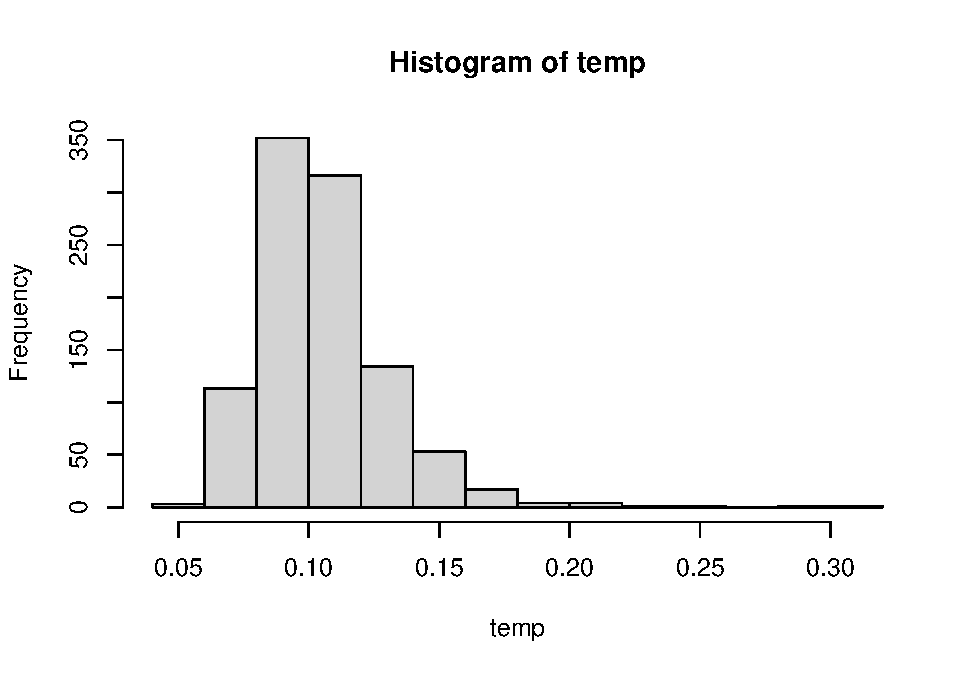
\includegraphics{03-maps_files/figure-latex/unnamed-chunk-5-1.pdf}

Then I will create a data frame with the mean indicator values and the SD.

\begin{Shaded}
\begin{Highlighting}[]
\FunctionTok{library}\NormalTok{(matrixStats)}
\CommentTok{\#\textgreater{} Warning: package \textquotesingle{}matrixStats\textquotesingle{} was built under R version}
\CommentTok{\#\textgreater{} 4.1.3}
\CommentTok{\#\textgreater{} }
\CommentTok{\#\textgreater{} Attaching package: \textquotesingle{}matrixStats\textquotesingle{}}
\CommentTok{\#\textgreater{} The following object is masked from \textquotesingle{}package:dplyr\textquotesingle{}:}
\CommentTok{\#\textgreater{} }
\CommentTok{\#\textgreater{}     count}
\NormalTok{jerv\_tbl }\OtherTok{\textless{}{-}} \FunctionTok{data.frame}\NormalTok{(}\StringTok{"raw2019"} \OtherTok{=} \FunctionTok{round}\NormalTok{(}\FunctionTok{rowMeans}\NormalTok{(myMat2019), }\DecValTok{2}\NormalTok{),}
                       \StringTok{"sd2019"}  \OtherTok{=} \FunctionTok{round}\NormalTok{(matrixStats}\SpecialCharTok{::}\FunctionTok{rowSds}\NormalTok{(myMat2019), }\DecValTok{2}\NormalTok{),}
                       \StringTok{"ref"}     \OtherTok{=} \FunctionTok{round}\NormalTok{(}\FunctionTok{rowMeans}\NormalTok{(myMatr), }\DecValTok{2}\NormalTok{))}
\NormalTok{jerv\_tbl}\SpecialCharTok{$}\NormalTok{scaled }\OtherTok{\textless{}{-}} \FunctionTok{round}\NormalTok{(jerv\_tbl}\SpecialCharTok{$}\NormalTok{raw2019}\SpecialCharTok{/}\NormalTok{jerv\_tbl}\SpecialCharTok{$}\NormalTok{ref, }\DecValTok{2}\NormalTok{)}
\NormalTok{jerv\_tbl}\SpecialCharTok{$}\NormalTok{cv }\OtherTok{\textless{}{-}} \FunctionTok{round}\NormalTok{(jerv\_tbl}\SpecialCharTok{$}\NormalTok{sd2019}\SpecialCharTok{/}\NormalTok{jerv\_tbl}\SpecialCharTok{$}\NormalTok{raw2019, }\DecValTok{2}\NormalTok{)}
\NormalTok{jerv\_tbl}\SpecialCharTok{$}\NormalTok{region }\OtherTok{\textless{}{-}}\NormalTok{ jerv}\SpecialCharTok{$}\NormalTok{indicatorValues}\SpecialCharTok{$}\StringTok{\textasciigrave{}}\AttributeTok{2019}\StringTok{\textasciigrave{}}\SpecialCharTok{$}\NormalTok{ICunitName}
\NormalTok{DT}\SpecialCharTok{::}\FunctionTok{datatable}\NormalTok{(jerv\_tbl)}
\end{Highlighting}
\end{Shaded}

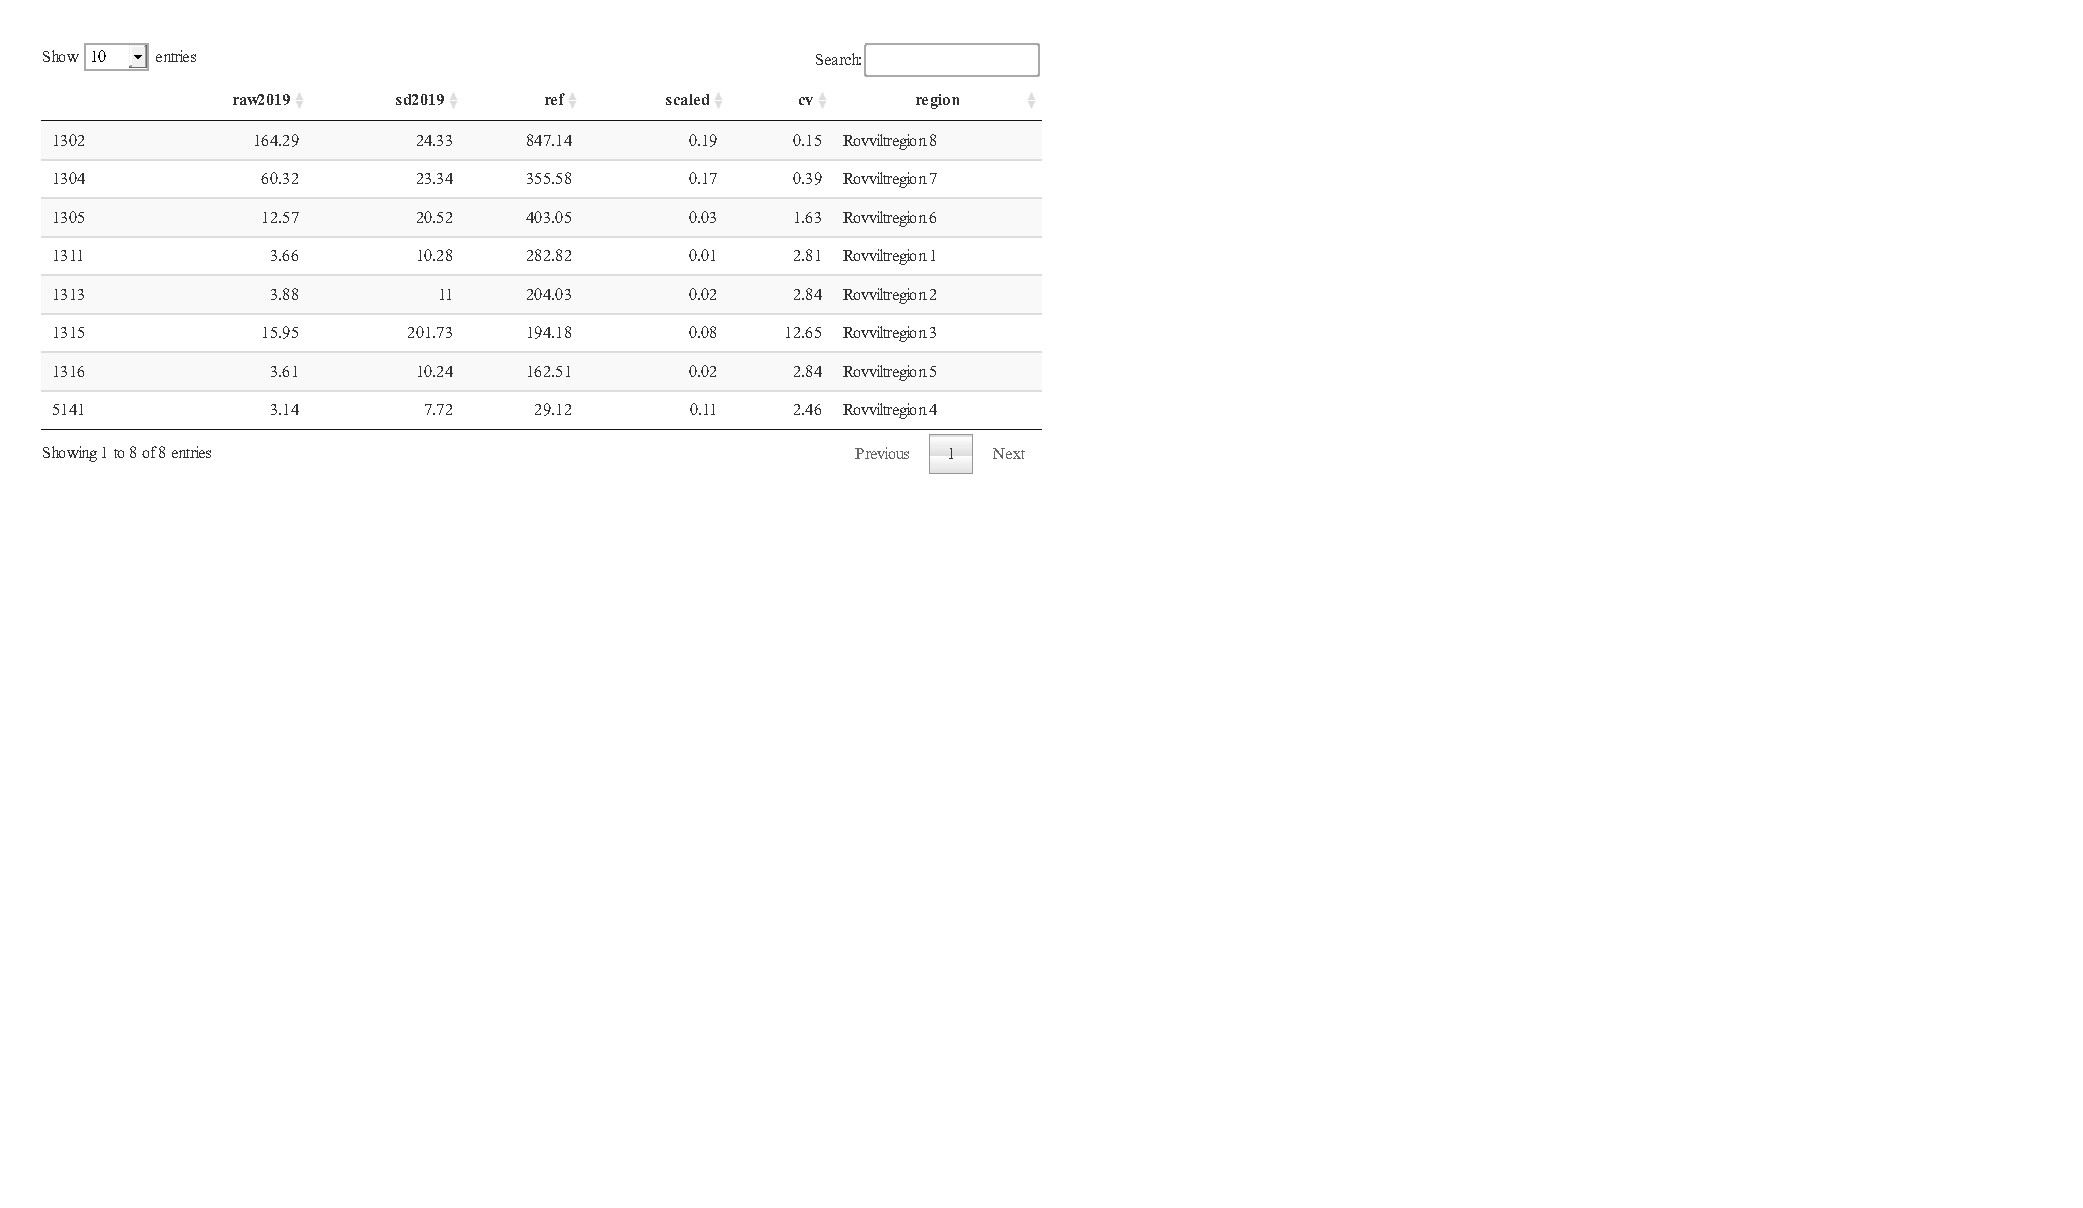
\includegraphics{03-maps_files/figure-latex/unnamed-chunk-6-1.pdf}
This is a special case maybe, because the sd is often larger than the mean.

Btw, we could use inbuilt NIcalc functions to get the indicator value, like I do below, but that will aggregate to regions, and we want to keep the original geometry.

\begin{Shaded}
\begin{Highlighting}[]
\NormalTok{jervComp }\OtherTok{\textless{}{-}}\NormalTok{ NIcalc}\SpecialCharTok{::}\FunctionTok{calculateIndex}\NormalTok{(}
  \AttributeTok{x       =}\NormalTok{ jerv,}
  \AttributeTok{nsim     =} \DecValTok{1000}\NormalTok{,}
  \AttributeTok{awBSunit =} \StringTok{"terrestrialArea"}\NormalTok{,}
  \AttributeTok{fids     =}\NormalTok{ F,    }\CommentTok{\# should fidelities be ignored in }
                   \CommentTok{\# the calculation of Wi?}
  \AttributeTok{tgroups  =}\NormalTok{ F, }\CommentTok{\# should grouping of indicators }
                   \CommentTok{\# into trophic and key indicator }
                   \CommentTok{\# groups be ignored}
  \AttributeTok{keys     =} \StringTok{"specialWeight"}\NormalTok{, }\CommentTok{\#"ignore",}
\NormalTok{)}
\CommentTok{\#\textgreater{} Indices for NIunits \textquotesingle{}wholeArea\textquotesingle{}, \textquotesingle{}E\textquotesingle{}, \textquotesingle{}S\textquotesingle{}, \textquotesingle{}W\textquotesingle{}, \textquotesingle{}C\textquotesingle{}, \textquotesingle{}N\textquotesingle{}}
\CommentTok{\#\textgreater{} and years \textquotesingle{}1990\textquotesingle{}, \textquotesingle{}2000\textquotesingle{}, \textquotesingle{}2010\textquotesingle{}, \textquotesingle{}2014\textquotesingle{}, \textquotesingle{}2019\textquotesingle{} will be calculated.}
\CommentTok{\#\textgreater{} The 30 index distributions will each be based on  1000 simulations.}
\CommentTok{\#\textgreater{} There are 8 ICunits with observations in data set \textquotesingle{}jerv\textquotesingle{}.}
\CommentTok{\#\textgreater{} }
\CommentTok{\#\textgreater{} Calculating weights that are the same for all years .....}
\CommentTok{\#\textgreater{} }
\CommentTok{\#\textgreater{} Sampling reference values .....}
\CommentTok{\#\textgreater{} }
\CommentTok{\#\textgreater{} Sampling and scaling indicator observations from  1990 .....}
\CommentTok{\#\textgreater{} }
\CommentTok{\#\textgreater{} Sampling and scaling indicator observations from  2000 .....}
\CommentTok{\#\textgreater{} }
\CommentTok{\#\textgreater{} Sampling and scaling indicator observations from  2010 .....}
\CommentTok{\#\textgreater{} }
\CommentTok{\#\textgreater{} Sampling and scaling indicator observations from  2014 .....}
\CommentTok{\#\textgreater{} }
\CommentTok{\#\textgreater{} Sampling and scaling indicator observations from  2019 .....}
\FunctionTok{plot}\NormalTok{(jervComp}\SpecialCharTok{$}\NormalTok{wholeArea)}
\end{Highlighting}
\end{Shaded}

\begin{figure}
\centering
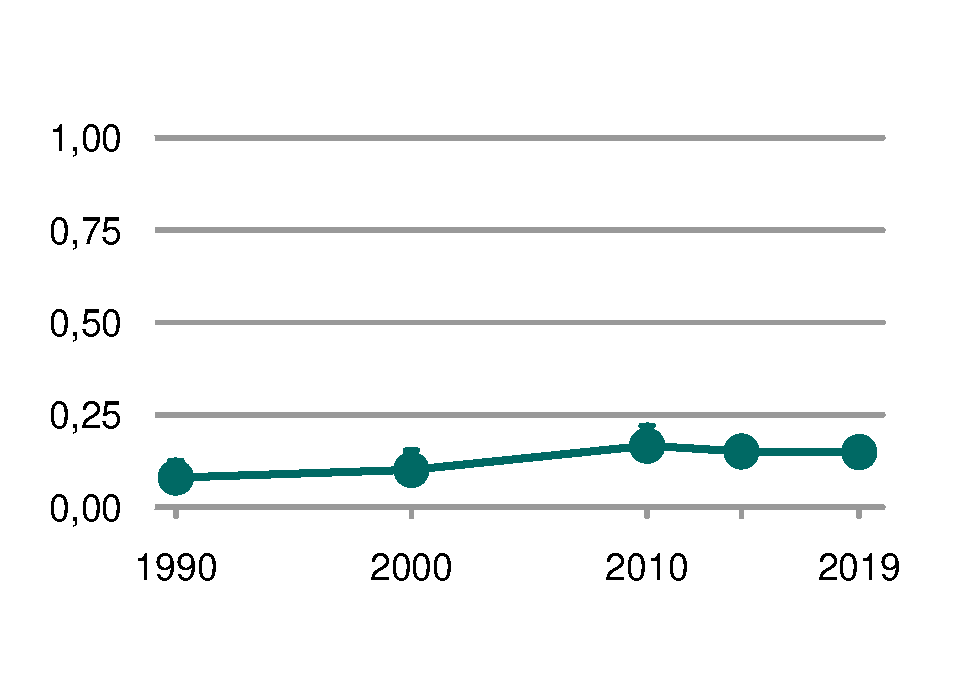
\includegraphics{03-maps_files/figure-latex/unnamed-chunk-7-1.pdf}
\caption{\label{fig:unnamed-chunk-7}The scaled indicator values for wolverine across Norway.}
\end{figure}

\hypertarget{get-geometries}{%
\subsubsection{Get geometries}\label{get-geometries}}

Then I can get the spatial geometries associated with the data. There are the so called rovviltregioner. There are eight of them. They are actually linked to the BS-units (municipalites), but we don't want to plot the outlines of the municipalities.
The geometries for the appropriate spatial units of each indicator can be downloaded in .json format via a previously created API for the nature index database: \url{https://ninweb08.nina.no/NaturindeksAPI/index.html}
To get the file for a specific indicator, one needs to enter the numerical indicator id under ``/api/Indicator/\{id\}/Areas'' and then click download. We then converted the .json file to shapefiles for use in R.

\begin{Shaded}
\begin{Highlighting}[]
\NormalTok{path }\OtherTok{\textless{}{-}} \StringTok{"P:/41201612\_naturindeks\_2021\_2023\_database\_og\_innsynslosning/Pilot\_Forbedring\_Innsynsløsning/Shapefiles/Jerv"}
\end{Highlighting}
\end{Shaded}

\begin{Shaded}
\begin{Highlighting}[]
\FunctionTok{library}\NormalTok{(sf)}
\CommentTok{\#\textgreater{} Warning: package \textquotesingle{}sf\textquotesingle{} was built under R version 4.1.3}
\CommentTok{\#\textgreater{} Linking to GEOS 3.10.2, GDAL 3.4.1, PROJ 7.2.1; sf\_use\_s2() is TRUE}
\NormalTok{rov }\OtherTok{\textless{}{-}}\NormalTok{ sf}\SpecialCharTok{::}\FunctionTok{read\_sf}\NormalTok{(path)}
\NormalTok{rov }\OtherTok{\textless{}{-}}\NormalTok{ sf}\SpecialCharTok{::}\FunctionTok{st\_make\_valid}\NormalTok{(rov)}
\NormalTok{rov }\OtherTok{\textless{}{-}}\NormalTok{ rov[rov}\SpecialCharTok{$}\NormalTok{area}\SpecialCharTok{!=}\StringTok{"DEF jerv"}\NormalTok{,]}
\end{Highlighting}
\end{Shaded}

Clip it against the outline of Norway to make it look more pretty

\begin{Shaded}
\begin{Highlighting}[]
\NormalTok{path }\OtherTok{\textless{}{-}} \StringTok{"data/outlineOfNorway\_EPSG25833.shp"}
\NormalTok{nor }\OtherTok{\textless{}{-}}\NormalTok{ sf}\SpecialCharTok{::}\FunctionTok{read\_sf}\NormalTok{(path)}
\NormalTok{nor }\OtherTok{\textless{}{-}} \FunctionTok{st\_transform}\NormalTok{(nor, }\AttributeTok{crs=}\FunctionTok{st\_crs}\NormalTok{(rov))}
\end{Highlighting}
\end{Shaded}

\begin{Shaded}
\begin{Highlighting}[]
\NormalTok{rov }\OtherTok{\textless{}{-}} \FunctionTok{st\_intersection}\NormalTok{(rov, nor)}
\CommentTok{\#\textgreater{} Warning: attribute variables are assumed to be spatially}
\CommentTok{\#\textgreater{} constant throughout all geometries}
\end{Highlighting}
\end{Shaded}

\hypertarget{link-data-and-geometries}{%
\subsubsection{Link data and geometries}\label{link-data-and-geometries}}

\begin{Shaded}
\begin{Highlighting}[]
\NormalTok{rov}\SpecialCharTok{$}\NormalTok{scaledIndicator }\OtherTok{\textless{}{-}}\NormalTok{ jerv\_tbl}\SpecialCharTok{$}\NormalTok{scaled[}\FunctionTok{match}\NormalTok{(rov}\SpecialCharTok{$}\NormalTok{area, jerv\_tbl}\SpecialCharTok{$}\NormalTok{region)]}
\NormalTok{rov}\SpecialCharTok{$}\NormalTok{cv }\OtherTok{\textless{}{-}}\NormalTok{ jerv\_tbl}\SpecialCharTok{$}\NormalTok{cv[}\FunctionTok{match}\NormalTok{(rov}\SpecialCharTok{$}\NormalTok{area, jerv\_tbl}\SpecialCharTok{$}\NormalTok{region)]}
\NormalTok{rov}\SpecialCharTok{$}\NormalTok{raw }\OtherTok{\textless{}{-}}\NormalTok{ jerv\_tbl}\SpecialCharTok{$}\NormalTok{raw2019[}\FunctionTok{match}\NormalTok{(rov}\SpecialCharTok{$}\NormalTok{area, jerv\_tbl}\SpecialCharTok{$}\NormalTok{region)]}
\end{Highlighting}
\end{Shaded}

\begin{Shaded}
\begin{Highlighting}[]
\FunctionTok{library}\NormalTok{(tmap)}
\CommentTok{\#\textgreater{} Warning: package \textquotesingle{}tmap\textquotesingle{} was built under R version 4.1.3}
\NormalTok{one }\OtherTok{\textless{}{-}} \FunctionTok{tm\_shape}\NormalTok{(rov)}\SpecialCharTok{+}
  \FunctionTok{tm\_polygons}\NormalTok{(}\AttributeTok{col=}\StringTok{"scaledIndicator"}\NormalTok{, }
              \AttributeTok{border.col =} \StringTok{"white"}\NormalTok{)}

\NormalTok{two }\OtherTok{\textless{}{-}} \FunctionTok{tm\_shape}\NormalTok{(rov)}\SpecialCharTok{+}
  \FunctionTok{tm\_polygons}\NormalTok{(}\AttributeTok{col=}\StringTok{"cv"}\NormalTok{, }
              \AttributeTok{border.col =} \StringTok{"white"}\NormalTok{)}

\NormalTok{three }\OtherTok{\textless{}{-}} \FunctionTok{tm\_shape}\NormalTok{(rov)}\SpecialCharTok{+}
  \FunctionTok{tm\_polygons}\NormalTok{(}\AttributeTok{col=}\StringTok{"raw"}\NormalTok{, }
              \AttributeTok{border.col =} \StringTok{"white"}\NormalTok{)}


\FunctionTok{tmap\_arrange}\NormalTok{(one, two, }
             \AttributeTok{widths =} \FunctionTok{c}\NormalTok{(.}\DecValTok{75}\NormalTok{, .}\DecValTok{25}\NormalTok{),}
             \AttributeTok{heights =} \FunctionTok{c}\NormalTok{(}\DecValTok{1}\NormalTok{, }\FloatTok{0.5}\NormalTok{))}
\end{Highlighting}
\end{Shaded}

\includegraphics{03-maps_files/figure-latex/unnamed-chunk-13-1.pdf}

\hypertarget{other-figures}{%
\chapter{Other figures}\label{other-figures}}

\hypertarget{gradient-density-plots-for-interactive-maps}{%
\section{Gradient density plots for interactive maps}\label{gradient-density-plots-for-interactive-maps}}

The maps presented on the webpage do not include any representation of uncertainty. One way of including that information without having to add additional (layers to the) maps would be to build on the interactive functions included so far and present a probability distribution for the given region and year. This could be displayed in the same box that currently appears when hovering over an area and displays area name and average indicator value.

To make these density plots, we use the previously simulated bootstrap samples, using Jerv as an example:

\begin{Shaded}
\begin{Highlighting}[]

\NormalTok{i }\OtherTok{\textless{}{-}} \StringTok{"Jerv"}
\NormalTok{bootStrp }\OtherTok{\textless{}{-}} \FunctionTok{readRDS}\NormalTok{(}\FunctionTok{paste0}\NormalTok{(}\StringTok{"data/"}\NormalTok{, i, }\StringTok{"\_bootstrapped\_scaled.rds"}\NormalTok{))}
\FunctionTok{head}\NormalTok{(bootStrp)}
\CommentTok{\#\textgreater{} \# A tibble: 6 x 4}
\CommentTok{\#\textgreater{}   ICunitID ICunitName      year  scaledIndicator}
\CommentTok{\#\textgreater{}   \textless{}chr\textgreater{}    \textless{}chr\textgreater{}           \textless{}chr\textgreater{}           \textless{}dbl\textgreater{}}
\CommentTok{\#\textgreater{} 1 1302     Rovviltregion 8 1990            0.194}
\CommentTok{\#\textgreater{} 2 1302     Rovviltregion 8 1990            0.233}
\CommentTok{\#\textgreater{} 3 1302     Rovviltregion 8 1990            0.190}
\CommentTok{\#\textgreater{} 4 1302     Rovviltregion 8 1990            0.207}
\CommentTok{\#\textgreater{} 5 1302     Rovviltregion 8 1990            0.199}
\CommentTok{\#\textgreater{} 6 1302     Rovviltregion 8 1990            0.164}
\end{Highlighting}
\end{Shaded}

I have considered forcing all indicator values \textgreater{} 1 to display as 1, but this messes up when plotting density functions. Still, this conversion is required for calculating the point estimate (median) and I therefore make a copy of the data in which no values are larger than 1.

\begin{Shaded}
\begin{Highlighting}[]
\NormalTok{bootStrp1 }\OtherTok{\textless{}{-}}\NormalTok{ bootStrp}
\NormalTok{bootStrp1}\SpecialCharTok{$}\NormalTok{scaledIndicator[}\FunctionTok{which}\NormalTok{(bootStrp1}\SpecialCharTok{$}\NormalTok{scaledIndicator }\SpecialCharTok{\textgreater{}} \DecValTok{1}\NormalTok{)] }\OtherTok{\textless{}{-}} \DecValTok{1}
\end{Highlighting}
\end{Shaded}

Next, we need to manually calculate the probability densities for the indicator values in each year and area. This is necessary for making density plots with a color gradient fill (but see further below for an alternative using the ``ggridges'' package which does not require this intermediate step).

\begin{Shaded}
\begin{Highlighting}[]
\NormalTok{years }\OtherTok{\textless{}{-}} \FunctionTok{unique}\NormalTok{(bootStrp}\SpecialCharTok{$}\NormalTok{year)}
\NormalTok{areas }\OtherTok{\textless{}{-}} \FunctionTok{unique}\NormalTok{(bootStrp}\SpecialCharTok{$}\NormalTok{ICunitName)}

\NormalTok{pDens }\OtherTok{\textless{}{-}} \FunctionTok{data.frame}\NormalTok{()}
\ControlFlowTok{for}\NormalTok{(t }\ControlFlowTok{in}\NormalTok{ years)\{}
  \ControlFlowTok{for}\NormalTok{(a }\ControlFlowTok{in}\NormalTok{ areas)\{}
    
\NormalTok{    bootStrp\_sub }\OtherTok{\textless{}{-}} \FunctionTok{subset}\NormalTok{(bootStrp, year }\SpecialCharTok{==}\NormalTok{ t }\SpecialCharTok{\&}\NormalTok{ ICunitName }\SpecialCharTok{==}\NormalTok{ a)}
    
\NormalTok{    pDens\_a\_t }\OtherTok{\textless{}{-}} \FunctionTok{data.frame}\NormalTok{(}
      \AttributeTok{ICunitName =}\NormalTok{ a,}
      \AttributeTok{year =}\NormalTok{ t, }
      \AttributeTok{x =} \FunctionTok{density}\NormalTok{(bootStrp\_sub}\SpecialCharTok{$}\NormalTok{scaledIndicator)}\SpecialCharTok{$}\NormalTok{x,}
      \AttributeTok{y =} \FunctionTok{density}\NormalTok{(bootStrp\_sub}\SpecialCharTok{$}\NormalTok{scaledIndicator)}\SpecialCharTok{$}\NormalTok{y}
\NormalTok{    )}
    
\NormalTok{    pDens }\OtherTok{\textless{}{-}} \FunctionTok{rbind}\NormalTok{(pDens, pDens\_a\_t)}
\NormalTok{  \}}
\NormalTok{\}}
\end{Highlighting}
\end{Shaded}

We can then proceed to plotting the probability density functions with a color gradient under the line:

\begin{Shaded}
\begin{Highlighting}[]

\CommentTok{\# Set maximum value (we will not plot beyond 4)}

\ControlFlowTok{for}\NormalTok{(t }\ControlFlowTok{in}\NormalTok{ years)\{}

  \CommentTok{\# Take data subsets for a given year}
\NormalTok{  bootStrp\_yr }\OtherTok{\textless{}{-}}\NormalTok{ bootStrp[}\FunctionTok{which}\NormalTok{(bootStrp}\SpecialCharTok{$}\NormalTok{year }\SpecialCharTok{==}\NormalTok{ t),]}
\NormalTok{  bootStrp1\_yr }\OtherTok{\textless{}{-}}\NormalTok{ bootStrp1[}\FunctionTok{which}\NormalTok{(bootStrp1}\SpecialCharTok{$}\NormalTok{year }\SpecialCharTok{==}\NormalTok{ t),]}
\NormalTok{  pDens\_yr }\OtherTok{\textless{}{-}}\NormalTok{ pDens[}\FunctionTok{which}\NormalTok{(pDens}\SpecialCharTok{$}\NormalTok{year }\SpecialCharTok{==}\NormalTok{ t),]}

  \CommentTok{\# Extract distribution medians}
\NormalTok{  sum\_values }\OtherTok{\textless{}{-}}\NormalTok{ bootStrp1\_yr }\SpecialCharTok{\%\textgreater{}\%} 
    \FunctionTok{group\_by}\NormalTok{(ICunitName) }\SpecialCharTok{\%\textgreater{}\%}
    \FunctionTok{summarise}\NormalTok{(}\AttributeTok{sumStat =} \FunctionTok{median}\NormalTok{(scaledIndicator)) }
  
  \CommentTok{\# Set maximum plotting value (never \textgreater{} 5) and mapping for custom color scale}
\NormalTok{  maxVal }\OtherTok{\textless{}{-}} \FunctionTok{ifelse}\NormalTok{(}\FunctionTok{max}\NormalTok{(pDens\_yr}\SpecialCharTok{$}\NormalTok{x) }\SpecialCharTok{\textgreater{}} \DecValTok{5}\NormalTok{, }\DecValTok{5}\NormalTok{, }\FunctionTok{max}\NormalTok{(pDens\_yr}\SpecialCharTok{$}\NormalTok{x))}
  
  \ControlFlowTok{if}\NormalTok{(maxVal }\SpecialCharTok{\textless{}} \DecValTok{1}\SpecialCharTok{+}\DecValTok{1}\SpecialCharTok{/}\DecValTok{9}\NormalTok{)\{}
\NormalTok{    valuesMap }\OtherTok{\textless{}{-}} \FunctionTok{c}\NormalTok{(}\SpecialCharTok{{-}}\FloatTok{0.1}\NormalTok{, }\FunctionTok{seq}\NormalTok{(}\DecValTok{0}\NormalTok{, }\DecValTok{1}\NormalTok{, }\AttributeTok{length.out =} \DecValTok{10}\NormalTok{))}
\NormalTok{    colorMap }\OtherTok{\textless{}{-}} \FunctionTok{c}\NormalTok{(}\StringTok{"\#1F8C81"}\NormalTok{, NIviz\_colours}\SpecialCharTok{$}\NormalTok{IndMap\_cols)}
\NormalTok{  \}}\ControlFlowTok{else}\NormalTok{\{}
\NormalTok{    valuesMap }\OtherTok{\textless{}{-}} \FunctionTok{c}\NormalTok{(}\SpecialCharTok{{-}}\FloatTok{0.1}\NormalTok{, }\FunctionTok{c}\NormalTok{(}\FunctionTok{seq}\NormalTok{(}\DecValTok{0}\NormalTok{, }\DecValTok{1}\NormalTok{, }\AttributeTok{length.out =} \DecValTok{10}\NormalTok{), maxVal)}\SpecialCharTok{/}\NormalTok{maxVal)}
\NormalTok{    colorMap }\OtherTok{\textless{}{-}} \FunctionTok{c}\NormalTok{(}\StringTok{"\#1F8C81"}\NormalTok{, NIviz\_colours}\SpecialCharTok{$}\NormalTok{IndMap\_cols, }\StringTok{"\#4B4BAF"}\NormalTok{)}
\NormalTok{  \}}
  
  \CommentTok{\# Plot densities}
  \FunctionTok{print}\NormalTok{(}
    \FunctionTok{ggplot}\NormalTok{(}\FunctionTok{subset}\NormalTok{(pDens\_yr, x }\SpecialCharTok{\textless{}=}\NormalTok{ maxVal), }\FunctionTok{aes}\NormalTok{(x, y)) }\SpecialCharTok{+} 
      \FunctionTok{geom\_segment}\NormalTok{(}\FunctionTok{aes}\NormalTok{(}\AttributeTok{xend =}\NormalTok{ x, }\AttributeTok{yend =} \DecValTok{0}\NormalTok{, }\AttributeTok{colour =}\NormalTok{ x)) }\SpecialCharTok{+} 
      \CommentTok{\#scale\_color\_NIviz\_c(name = "IndMap\_cols") + }
      \FunctionTok{scale\_colour\_gradientn}\NormalTok{(}\AttributeTok{colours =}\NormalTok{ colorMap,}
                             \AttributeTok{values =}\NormalTok{ valuesMap,}
                             \AttributeTok{limits =} \FunctionTok{c}\NormalTok{(}\SpecialCharTok{{-}}\FloatTok{0.01}\NormalTok{, }\FunctionTok{ifelse}\NormalTok{(maxVal }\SpecialCharTok{\textless{}} \DecValTok{1}\NormalTok{, }\DecValTok{1}\NormalTok{, maxVal))) }\SpecialCharTok{+}
      \FunctionTok{ggtitle}\NormalTok{(}\FunctionTok{paste0}\NormalTok{(i, }\StringTok{" ("}\NormalTok{, t, }\StringTok{")"}\NormalTok{)) }\SpecialCharTok{+}
      \FunctionTok{xlab}\NormalTok{(}\StringTok{"Value"}\NormalTok{) }\SpecialCharTok{+} 
      \FunctionTok{geom\_vline}\NormalTok{(}\AttributeTok{data =}\NormalTok{ sum\_values, }\FunctionTok{aes}\NormalTok{(}\AttributeTok{xintercept =}\NormalTok{ sumStat)) }\SpecialCharTok{+} 
      \FunctionTok{facet\_wrap}\NormalTok{(}\SpecialCharTok{\textasciitilde{}}\NormalTok{ ICunitName, }\AttributeTok{scales =} \StringTok{\textquotesingle{}free\textquotesingle{}}\NormalTok{) }\SpecialCharTok{+} 
      \FunctionTok{theme\_classic}\NormalTok{() }\SpecialCharTok{+} 
      \FunctionTok{theme}\NormalTok{(}\AttributeTok{strip.background =} \FunctionTok{element\_blank}\NormalTok{(), }
            \AttributeTok{legend.title =} \FunctionTok{element\_blank}\NormalTok{(),}
            \AttributeTok{axis.line.y =} \FunctionTok{element\_blank}\NormalTok{(), }\AttributeTok{axis.ticks.y =} \FunctionTok{element\_blank}\NormalTok{(),}
            \AttributeTok{axis.text.y =} \FunctionTok{element\_blank}\NormalTok{(), }\AttributeTok{axis.title.y =} \FunctionTok{element\_blank}\NormalTok{())}
\NormalTok{  )}
\NormalTok{\}}
\end{Highlighting}
\end{Shaded}

\includegraphics{04-other_figures_files/figure-latex/unnamed-chunk-4-1.pdf} 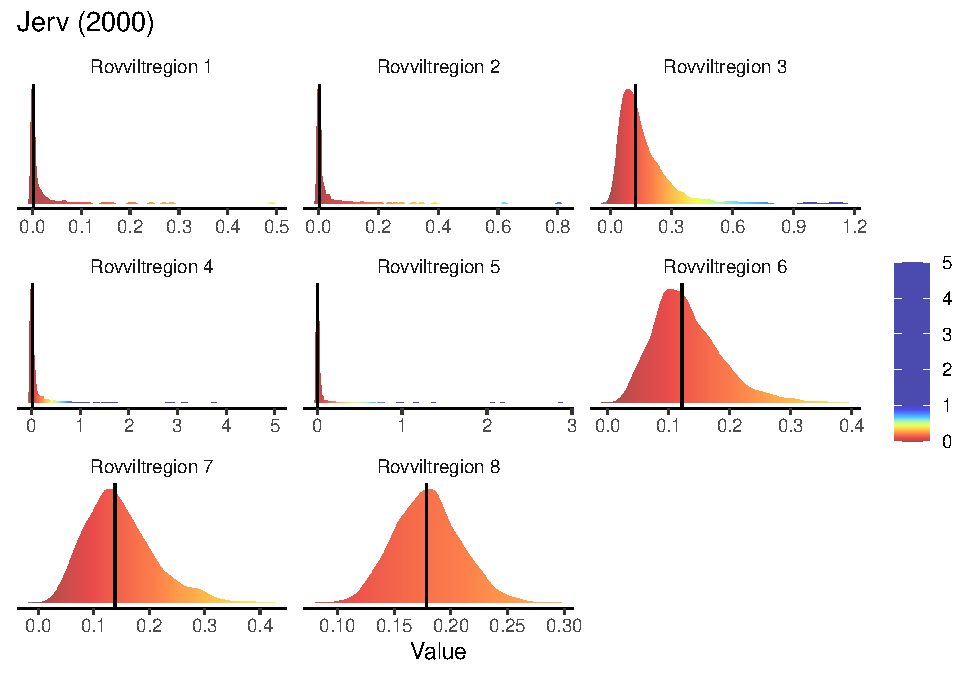
\includegraphics{04-other_figures_files/figure-latex/unnamed-chunk-4-2.pdf} 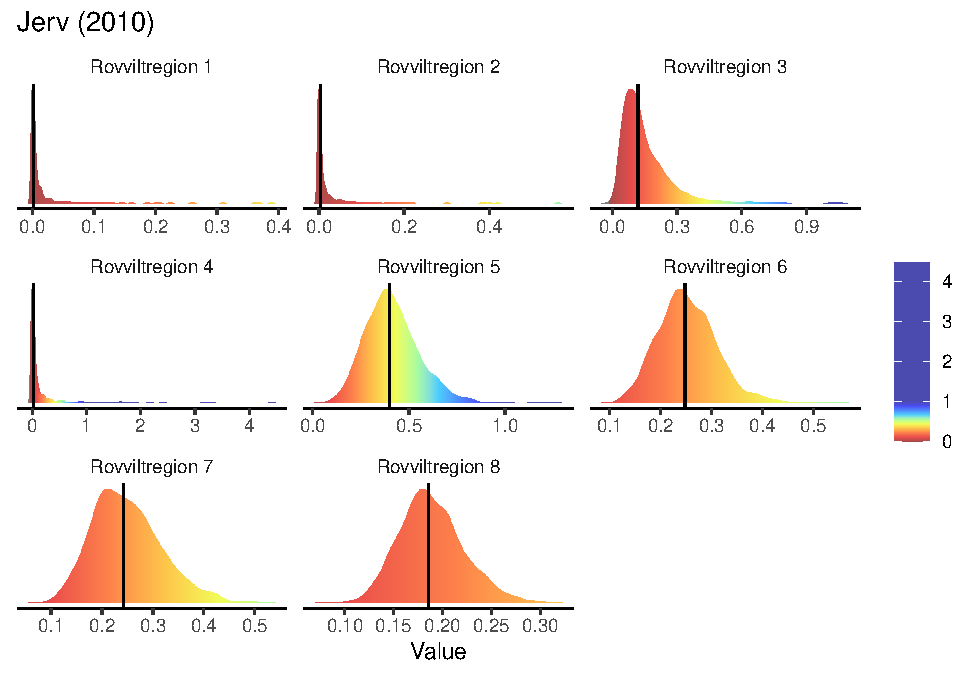
\includegraphics{04-other_figures_files/figure-latex/unnamed-chunk-4-3.pdf} 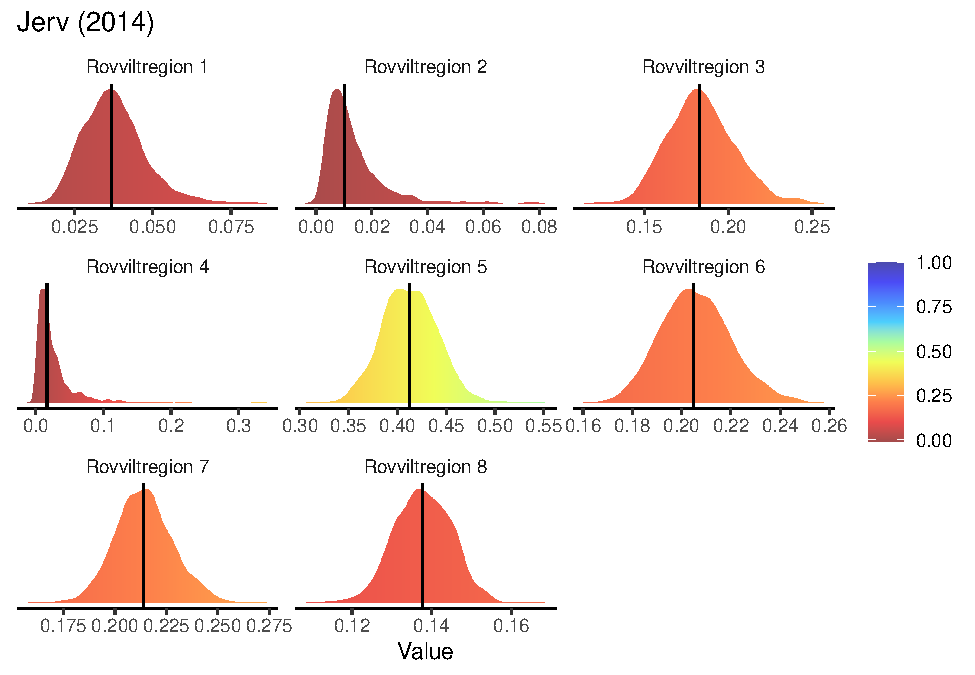
\includegraphics{04-other_figures_files/figure-latex/unnamed-chunk-4-4.pdf} 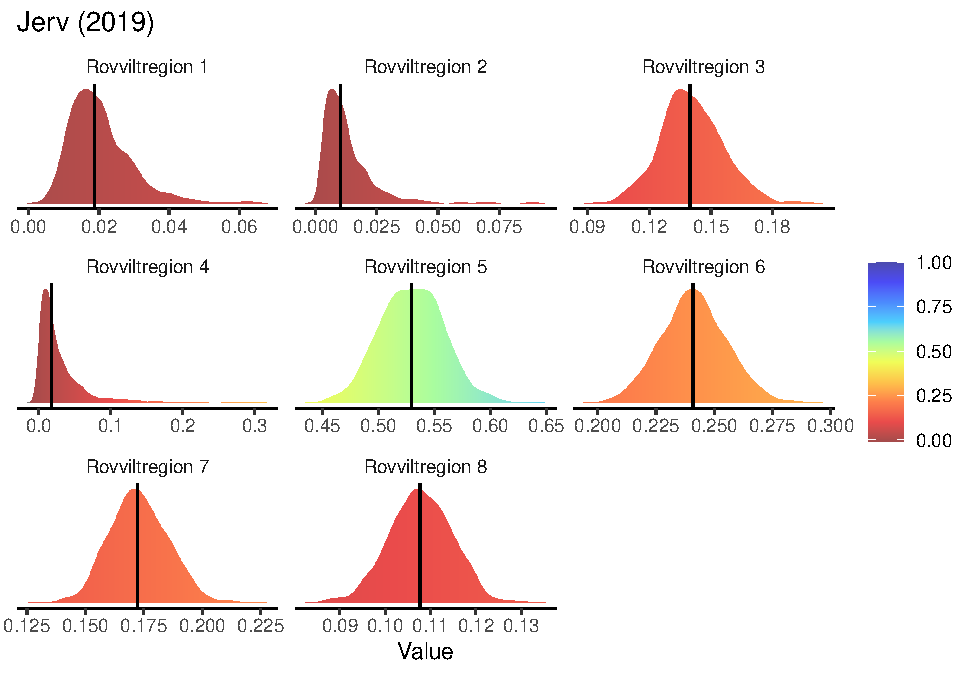
\includegraphics{04-other_figures_files/figure-latex/unnamed-chunk-4-5.pdf}

Gradient density plots might also be useful for other types of visualization of indicator and index data. For example, there is a very attractive way of using ridgeplots for visualizing time series inclusing uncertainty. Could look something like this:

\begin{Shaded}
\begin{Highlighting}[]

\ControlFlowTok{for}\NormalTok{(a }\ControlFlowTok{in}\NormalTok{ areas)\{}
  
  \CommentTok{\# Take data subsets for a given area}
\NormalTok{  bootStrp\_ar }\OtherTok{\textless{}{-}}\NormalTok{ bootStrp[}\FunctionTok{which}\NormalTok{(bootStrp}\SpecialCharTok{$}\NormalTok{ICunitName }\SpecialCharTok{==}\NormalTok{ a),]}
\NormalTok{  pDens\_ar }\OtherTok{\textless{}{-}}\NormalTok{ pDens[}\FunctionTok{which}\NormalTok{(pDens}\SpecialCharTok{$}\NormalTok{ICunitName }\SpecialCharTok{==}\NormalTok{ a),]}
  
  \CommentTok{\# Set maximum plotting value (never \textgreater{} 5) and mapping for custom color scale}
\NormalTok{  maxVal }\OtherTok{\textless{}{-}} \FunctionTok{ifelse}\NormalTok{(}\FunctionTok{max}\NormalTok{(pDens\_ar}\SpecialCharTok{$}\NormalTok{x) }\SpecialCharTok{\textgreater{}} \DecValTok{5}\NormalTok{, }\DecValTok{5}\NormalTok{, }\FunctionTok{max}\NormalTok{(pDens\_ar}\SpecialCharTok{$}\NormalTok{x))}
  
  \ControlFlowTok{if}\NormalTok{(maxVal }\SpecialCharTok{\textless{}} \DecValTok{1}\SpecialCharTok{+}\DecValTok{1}\SpecialCharTok{/}\DecValTok{9}\NormalTok{)\{}
\NormalTok{    valuesMap }\OtherTok{\textless{}{-}} \FunctionTok{c}\NormalTok{(}\SpecialCharTok{{-}}\FloatTok{0.1}\NormalTok{, }\FunctionTok{seq}\NormalTok{(}\DecValTok{0}\NormalTok{, }\DecValTok{1}\NormalTok{, }\AttributeTok{length.out =} \DecValTok{10}\NormalTok{))}
\NormalTok{    colorMap }\OtherTok{\textless{}{-}} \FunctionTok{c}\NormalTok{(}\StringTok{"\#1F8C81"}\NormalTok{, NIviz\_colours}\SpecialCharTok{$}\NormalTok{IndMap\_cols)}
\NormalTok{  \}}\ControlFlowTok{else}\NormalTok{\{}
\NormalTok{    valuesMap }\OtherTok{\textless{}{-}} \FunctionTok{c}\NormalTok{(}\SpecialCharTok{{-}}\FloatTok{0.1}\NormalTok{, }\FunctionTok{c}\NormalTok{(}\FunctionTok{seq}\NormalTok{(}\DecValTok{0}\NormalTok{, }\DecValTok{1}\NormalTok{, }\AttributeTok{length.out =} \DecValTok{10}\NormalTok{), maxVal)}\SpecialCharTok{/}\NormalTok{maxVal)}
\NormalTok{    colorMap }\OtherTok{\textless{}{-}} \FunctionTok{c}\NormalTok{(}\StringTok{"\#1F8C81"}\NormalTok{, NIviz\_colours}\SpecialCharTok{$}\NormalTok{IndMap\_cols, }\StringTok{"\#4B4BAF"}\NormalTok{)}
\NormalTok{  \}}
  
  \CommentTok{\# Plot densities}
  \FunctionTok{print}\NormalTok{(}
  
  \FunctionTok{ggplot}\NormalTok{(}\FunctionTok{subset}\NormalTok{(bootStrp\_ar, scaledIndicator }\SpecialCharTok{\textless{}=}\NormalTok{ maxVal), }\FunctionTok{aes}\NormalTok{(}\AttributeTok{x =}\NormalTok{ scaledIndicator, }\AttributeTok{y =}\NormalTok{ year, }\AttributeTok{fill =} \FunctionTok{stat}\NormalTok{(x))) }\SpecialCharTok{+}
    \FunctionTok{geom\_density\_ridges\_gradient}\NormalTok{(}\AttributeTok{scale =} \DecValTok{5}\NormalTok{, }\AttributeTok{rel\_min\_height =} \FloatTok{0.01}\NormalTok{, }\AttributeTok{quantile\_lines =} \ConstantTok{TRUE}\NormalTok{, }\AttributeTok{quantiles =} \DecValTok{2}\NormalTok{) }\SpecialCharTok{+} 
    \FunctionTok{scale\_fill\_gradientn}\NormalTok{(}\AttributeTok{colours =}\NormalTok{ colorMap,}
                         \AttributeTok{values =}\NormalTok{ valuesMap,}
                         \AttributeTok{limits =} \FunctionTok{c}\NormalTok{(}\SpecialCharTok{{-}}\FloatTok{0.02}\NormalTok{, }\FunctionTok{ifelse}\NormalTok{(maxVal }\SpecialCharTok{\textless{}} \DecValTok{1}\NormalTok{, }\DecValTok{1}\NormalTok{, maxVal))) }\SpecialCharTok{+}
    \FunctionTok{ggtitle}\NormalTok{(}\FunctionTok{paste0}\NormalTok{(i, }\StringTok{" ("}\NormalTok{, a, }\StringTok{")"}\NormalTok{)) }\SpecialCharTok{+} 
    \FunctionTok{xlab}\NormalTok{(}\StringTok{"Scaled indicator value"}\NormalTok{) }\SpecialCharTok{+} \FunctionTok{ylab}\NormalTok{(}\StringTok{""}\NormalTok{) }\SpecialCharTok{+} 
    \FunctionTok{theme\_classic}\NormalTok{() }\SpecialCharTok{+} 
    \FunctionTok{theme}\NormalTok{(}\AttributeTok{legend.title =} \FunctionTok{element\_blank}\NormalTok{(), }\AttributeTok{plot.title =} \FunctionTok{element\_text}\NormalTok{(}\AttributeTok{hjust =} \FloatTok{0.5}\NormalTok{),}
          \AttributeTok{axis.line.y =} \FunctionTok{element\_blank}\NormalTok{(), }\AttributeTok{axis.ticks.y =} \FunctionTok{element\_blank}\NormalTok{(),}
          \AttributeTok{panel.grid.major.y =} \FunctionTok{element\_line}\NormalTok{(}\AttributeTok{color =} \StringTok{"grey80"}\NormalTok{))}
\NormalTok{  )}
  
\NormalTok{\}}
\CommentTok{\#\textgreater{} Picking joint bandwidth of 0.00457}
\end{Highlighting}
\end{Shaded}

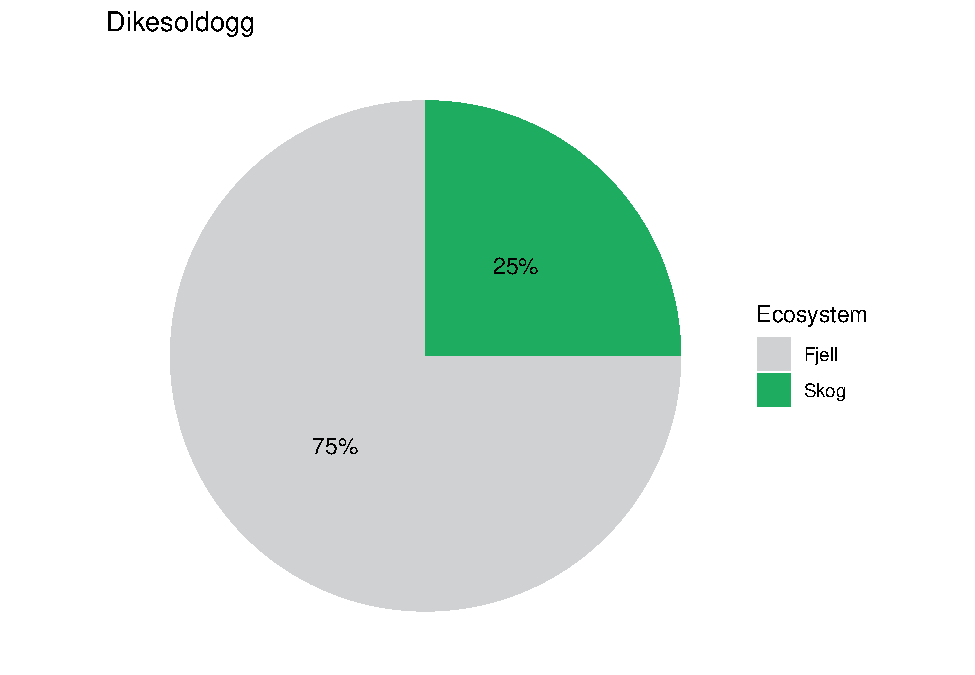
\includegraphics{04-other_figures_files/figure-latex/unnamed-chunk-5-1.pdf}

\begin{verbatim}
#> Picking joint bandwidth of 0.00947
\end{verbatim}

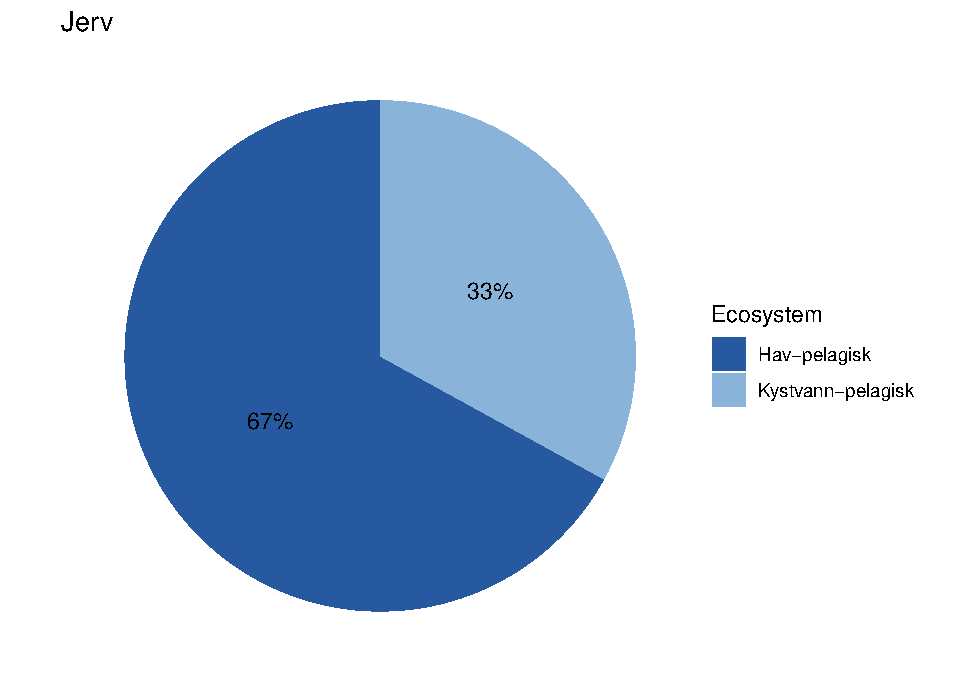
\includegraphics{04-other_figures_files/figure-latex/unnamed-chunk-5-2.pdf}

\begin{verbatim}
#> Picking joint bandwidth of 0.00715
\end{verbatim}

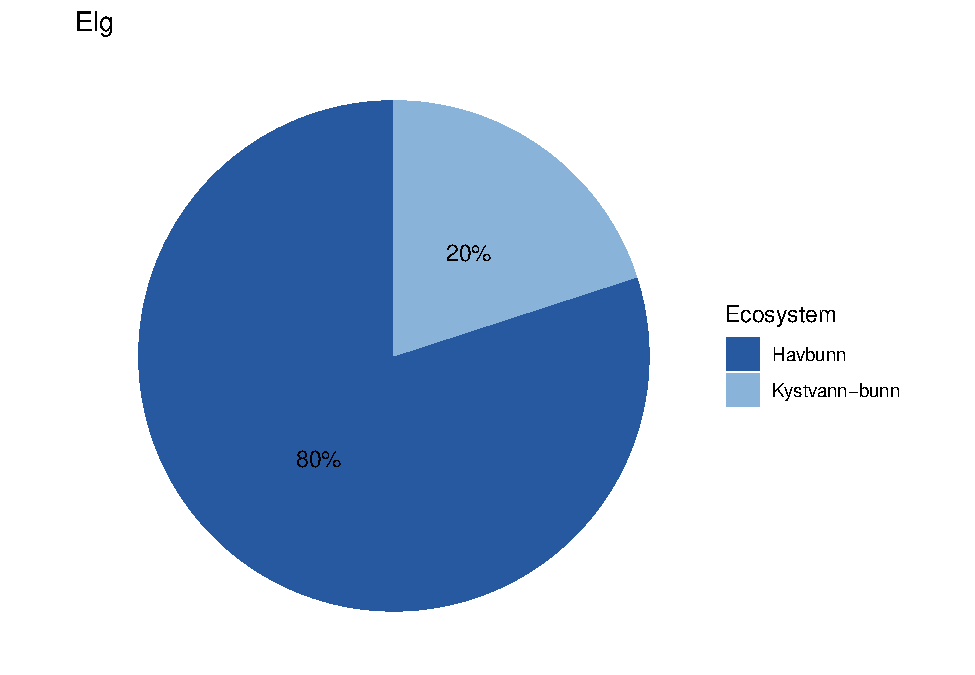
\includegraphics{04-other_figures_files/figure-latex/unnamed-chunk-5-3.pdf}

\begin{verbatim}
#> Picking joint bandwidth of 0.00184
\end{verbatim}

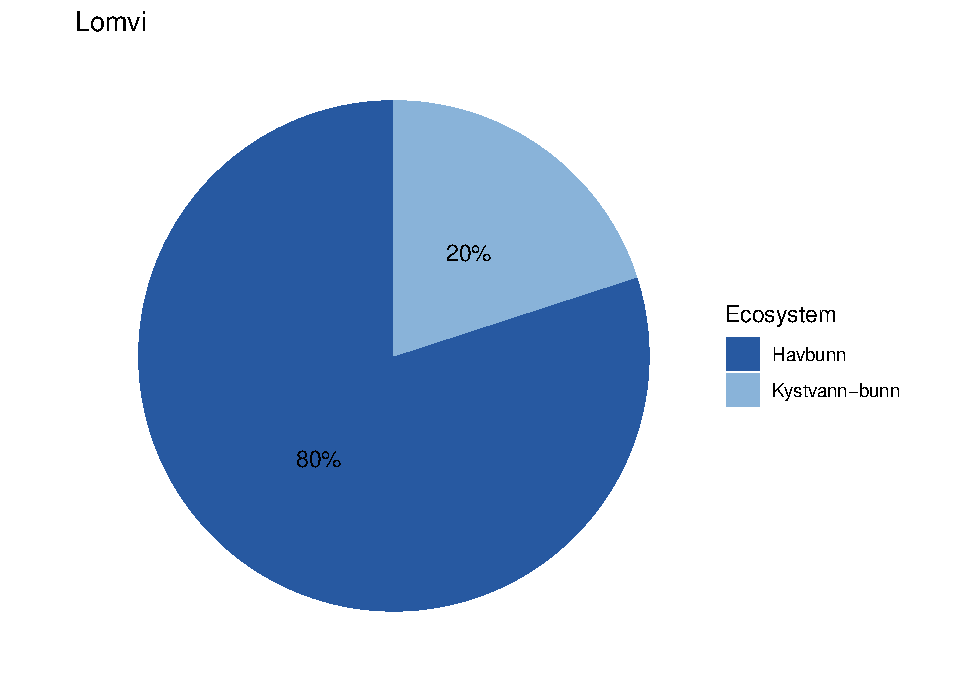
\includegraphics{04-other_figures_files/figure-latex/unnamed-chunk-5-4.pdf}

\begin{verbatim}
#> Picking joint bandwidth of 0.00215
\end{verbatim}

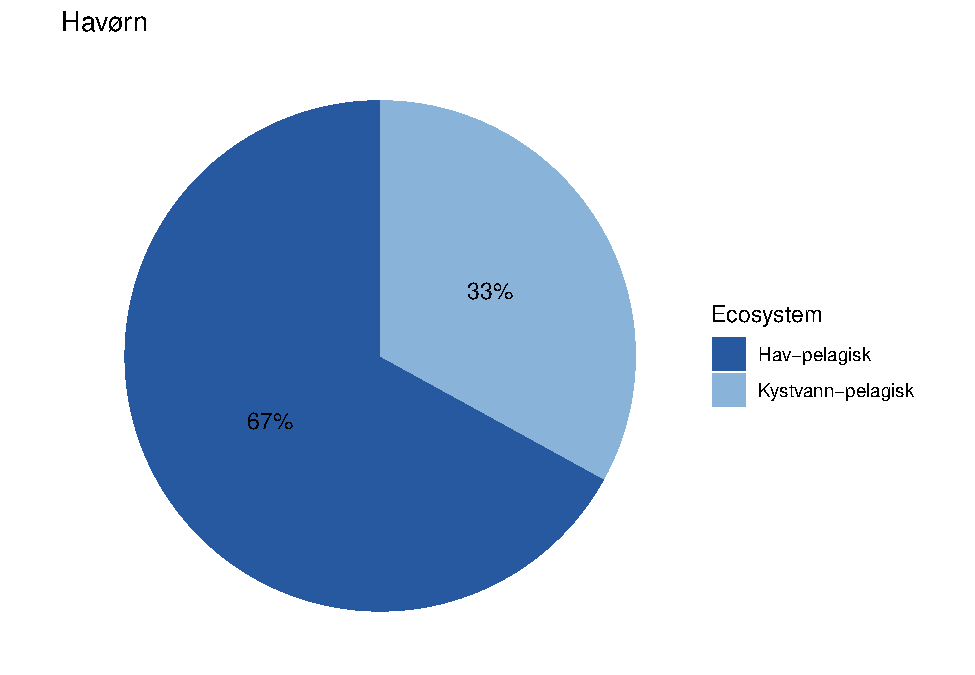
\includegraphics{04-other_figures_files/figure-latex/unnamed-chunk-5-5.pdf}

\begin{verbatim}
#> Picking joint bandwidth of 0.0101
\end{verbatim}

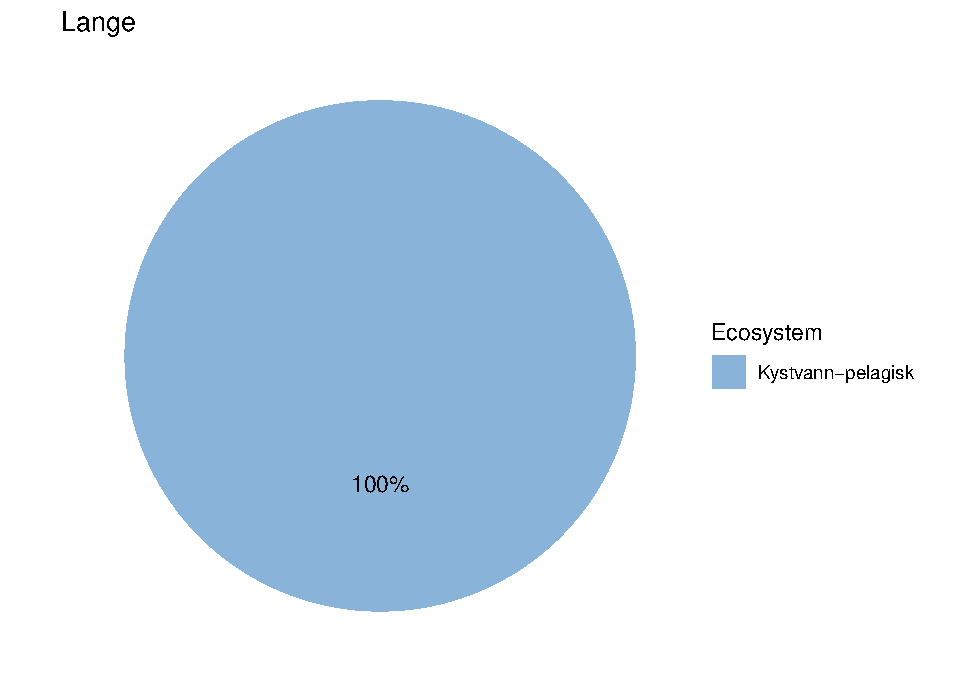
\includegraphics{04-other_figures_files/figure-latex/unnamed-chunk-5-6.pdf}

\begin{verbatim}
#> Picking joint bandwidth of 0.00966
\end{verbatim}

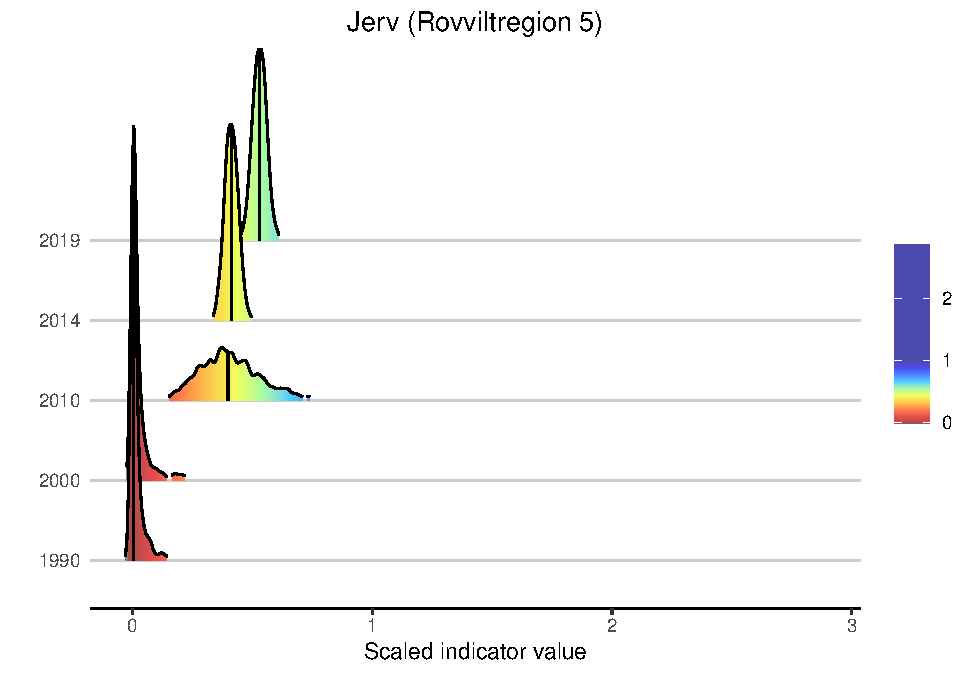
\includegraphics{04-other_figures_files/figure-latex/unnamed-chunk-5-7.pdf}

\begin{verbatim}
#> Picking joint bandwidth of 0.0112
\end{verbatim}

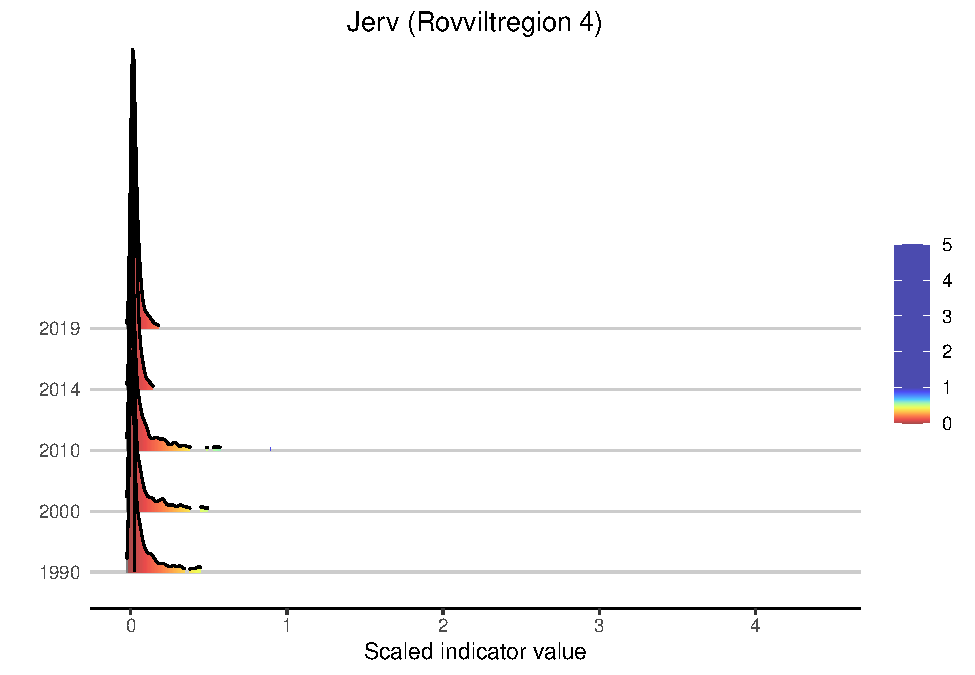
\includegraphics{04-other_figures_files/figure-latex/unnamed-chunk-5-8.pdf}

\hypertarget{ecosystem-fidelity}{%
\section{Ecosystem fidelity}\label{ecosystem-fidelity}}

All indicators are assigned to at least one ecosystem, but a fair number of them are assigned to multiple ecosystems by means of proportions. Wolverine (Jerv), for example, is assigned with 25\% to forest and and 75\% to mountain. This basic information could easily be displayed on each indicator's page on naturindeks.no.

The relevant information is found in the assembled indicator data under \$indicators:

\begin{Shaded}
\begin{Highlighting}[]

\NormalTok{i }\OtherTok{\textless{}{-}} \StringTok{"jerv"}
\NormalTok{indexData }\OtherTok{\textless{}{-}} \FunctionTok{readRDS}\NormalTok{(}\FunctionTok{paste0}\NormalTok{(}\StringTok{"data/"}\NormalTok{, i, }\StringTok{"\_assemebled.rds"}\NormalTok{))}

\FunctionTok{str}\NormalTok{(indexData}\SpecialCharTok{$}\NormalTok{indicators)}
\CommentTok{\#\textgreater{} \textquotesingle{}data.frame\textquotesingle{}:    1 obs. of  9 variables:}
\CommentTok{\#\textgreater{}  $ id               : num 88}
\CommentTok{\#\textgreater{}  $ name             : chr "Jerv"}
\CommentTok{\#\textgreater{}  $ keyElement       : logi FALSE}
\CommentTok{\#\textgreater{}  $ functionalGroup  : chr "Topp{-}predator generalist"}
\CommentTok{\#\textgreater{}  $ functionalGroupId: num 8}
\CommentTok{\#\textgreater{}  $ scalingModel     : chr "Low"}
\CommentTok{\#\textgreater{}  $ scalingModelId   : num 1}
\CommentTok{\#\textgreater{}  $ Fjell            : num 75}
\CommentTok{\#\textgreater{}  $ Skog             : num 25}
\end{Highlighting}
\end{Shaded}

Any ecosystem type relevant to a specific indicator appears as a separate column in this dataframe, and contains a value representing the \% fidelity to that ecosystem type.

Using separately stored information on available ecosystem types, we can assemble this data for all of our example indicators:

\begin{Shaded}
\begin{Highlighting}[]
\CommentTok{\# Load ecosystem info}
\NormalTok{EcoSysInfo }\OtherTok{\textless{}{-}} \FunctionTok{readRDS}\NormalTok{(}\StringTok{"data/EcosystemInfo.rds"}\NormalTok{)}

\CommentTok{\# Indicator list}
\NormalTok{indicator }\OtherTok{\textless{}{-}} \FunctionTok{c}\NormalTok{(}\StringTok{"Dikesoldogg"}\NormalTok{,}
               \StringTok{"Jerv"}\NormalTok{,}
               \StringTok{"Elg"}\NormalTok{,}
               \StringTok{"Lomvi"}\NormalTok{,}
               \StringTok{"Havørn"}\NormalTok{,}
               \StringTok{"Lange"}\NormalTok{)}

\CommentTok{\# Assemble fidelity data}
\NormalTok{fidData }\OtherTok{\textless{}{-}} \FunctionTok{data.frame}\NormalTok{()}

\ControlFlowTok{for}\NormalTok{(i }\ControlFlowTok{in} \DecValTok{1}\SpecialCharTok{:}\FunctionTok{length}\NormalTok{(indicator))\{}
  
\NormalTok{  indexData }\OtherTok{\textless{}{-}} \FunctionTok{readRDS}\NormalTok{(}\FunctionTok{paste0}\NormalTok{(}\StringTok{"data/"}\NormalTok{, indicator[i], }\StringTok{"\_assemebled.rds"}\NormalTok{))}
  
\NormalTok{  ColIdx }\OtherTok{\textless{}{-}} \FunctionTok{which}\NormalTok{(}\FunctionTok{names}\NormalTok{(indexData}\SpecialCharTok{$}\NormalTok{indicators) }\SpecialCharTok{\%in\%}\NormalTok{ EcoSysInfo}\SpecialCharTok{$}\NormalTok{ecosystem)}

\NormalTok{  fidDataI }\OtherTok{\textless{}{-}} \FunctionTok{data.frame}\NormalTok{(}
    \AttributeTok{indicator =}\NormalTok{ indicator[i],}
    \AttributeTok{ecosystem =} \FunctionTok{names}\NormalTok{(indexData}\SpecialCharTok{$}\NormalTok{indicators)[ColIdx],}
    \AttributeTok{fidelity =} \FunctionTok{unname}\NormalTok{(}\FunctionTok{as.numeric}\NormalTok{(indexData}\SpecialCharTok{$}\NormalTok{indicators[,ColIdx])))}
  
\NormalTok{  fidData }\OtherTok{\textless{}{-}} \FunctionTok{rbind}\NormalTok{(fidData, fidDataI)}
\NormalTok{\}}
\end{Highlighting}
\end{Shaded}

This gives us a dataframe with all indicators and their fidelity to different ecosystems:

\begin{Shaded}
\begin{Highlighting}[]
\FunctionTok{print}\NormalTok{(fidData)}
\CommentTok{\#\textgreater{}     indicator         ecosystem fidelity}
\CommentTok{\#\textgreater{} 1 Dikesoldogg           Våtmark      100}
\CommentTok{\#\textgreater{} 2        Jerv             Fjell       75}
\CommentTok{\#\textgreater{} 3        Jerv              Skog       25}
\CommentTok{\#\textgreater{} 4         Elg              Skog      100}
\CommentTok{\#\textgreater{} 5       Lomvi      Hav{-}pelagisk       67}
\CommentTok{\#\textgreater{} 6       Lomvi Kystvann{-}pelagisk       33}
\CommentTok{\#\textgreater{} 7      Havørn Kystvann{-}pelagisk      100}
\CommentTok{\#\textgreater{} 8       Lange           Havbunn       80}
\CommentTok{\#\textgreater{} 9       Lange     Kystvann{-}bunn       20}
\end{Highlighting}
\end{Shaded}

Before plotting, we match the integer ecosystem IDs to make sure the colour mapping works correctly:

\begin{Shaded}
\begin{Highlighting}[]
\NormalTok{fidData }\OtherTok{\textless{}{-}} \FunctionTok{merge}\NormalTok{(fidData, EcoSysInfo, }\AttributeTok{all.x =} \ConstantTok{TRUE}\NormalTok{)}
\end{Highlighting}
\end{Shaded}

Next, we'll visualize this information for each indicator by means of pie charts.

\begin{Shaded}
\begin{Highlighting}[]
\NormalTok{EcoSys\_cols }\OtherTok{\textless{}{-}}\NormalTok{ NIviz\_colours}\SpecialCharTok{$}\NormalTok{EcoSys\_cols[}\DecValTok{1}\SpecialCharTok{:}\DecValTok{11}\NormalTok{]}
\FunctionTok{names}\NormalTok{(EcoSys\_cols) }\OtherTok{\textless{}{-}}\NormalTok{ EcoSysInfo}\SpecialCharTok{$}\NormalTok{ecosystem}

\ControlFlowTok{for}\NormalTok{(i }\ControlFlowTok{in} \DecValTok{1}\SpecialCharTok{:}\FunctionTok{length}\NormalTok{(indicator))\{}
  
\NormalTok{  sub\_fidData }\OtherTok{\textless{}{-}}\NormalTok{ fidData[}\FunctionTok{which}\NormalTok{(fidData}\SpecialCharTok{$}\NormalTok{indicator }\SpecialCharTok{==}\NormalTok{ indicator[i]),]}
  
  \FunctionTok{print}\NormalTok{(}
    \FunctionTok{ggplot}\NormalTok{(sub\_fidData, }\FunctionTok{aes}\NormalTok{(}\AttributeTok{x =} \StringTok{""}\NormalTok{, }\AttributeTok{y =}\NormalTok{ fidelity, }\AttributeTok{fill =} \FunctionTok{fct\_inorder}\NormalTok{(ecosystem))) }\SpecialCharTok{+}
    \FunctionTok{ggtitle}\NormalTok{(indicator[i]) }\SpecialCharTok{+} 
    \FunctionTok{geom\_bar}\NormalTok{(}\AttributeTok{stat =} \StringTok{"identity"}\NormalTok{) }\SpecialCharTok{+}
    \FunctionTok{geom\_text}\NormalTok{(}\FunctionTok{aes}\NormalTok{(}\AttributeTok{label =} \FunctionTok{paste0}\NormalTok{(fidelity, }\StringTok{"\%"}\NormalTok{)),}
              \AttributeTok{position =} \FunctionTok{position\_stack}\NormalTok{(}\AttributeTok{vjust =} \FloatTok{0.5}\NormalTok{)) }\SpecialCharTok{+}
    \FunctionTok{coord\_polar}\NormalTok{(}\AttributeTok{theta =} \StringTok{"y"}\NormalTok{) }\SpecialCharTok{+}
    \FunctionTok{scale\_fill\_manual}\NormalTok{(}\AttributeTok{name =} \StringTok{"Økosystem"}\NormalTok{, }\AttributeTok{values =}\NormalTok{ EcoSys\_cols[}\FunctionTok{which}\NormalTok{(}\FunctionTok{names}\NormalTok{(EcoSys\_cols) }\SpecialCharTok{\%in\%}\NormalTok{ sub\_fidData}\SpecialCharTok{$}\NormalTok{ecosystem)]) }\SpecialCharTok{+} 
    \FunctionTok{theme\_void}\NormalTok{()}
\NormalTok{  )}

\NormalTok{\}}
\end{Highlighting}
\end{Shaded}

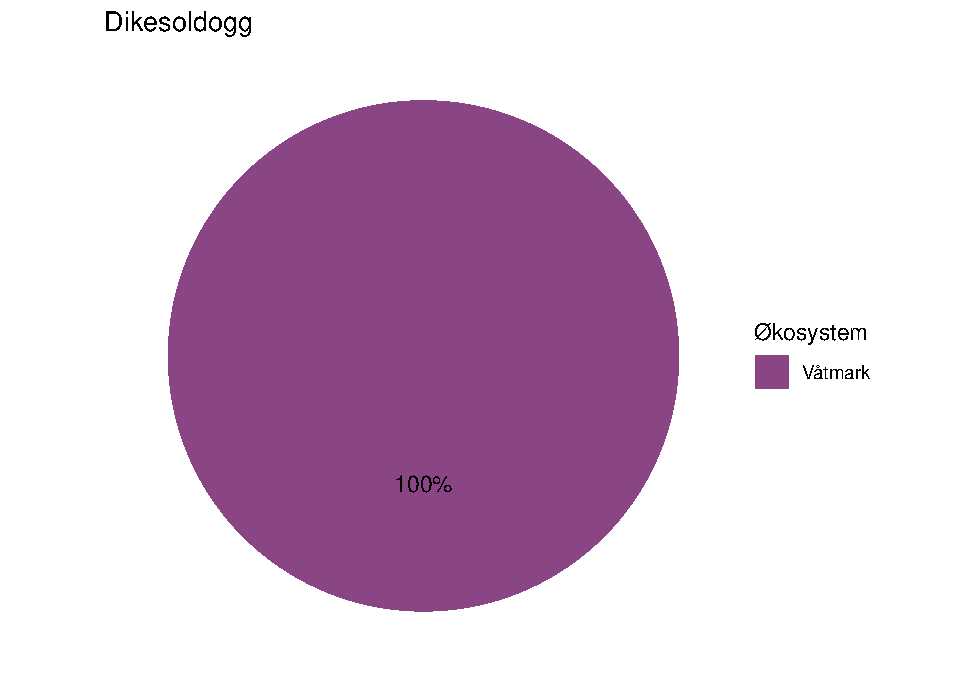
\includegraphics{04-other_figures_files/figure-latex/unnamed-chunk-10-1.pdf} 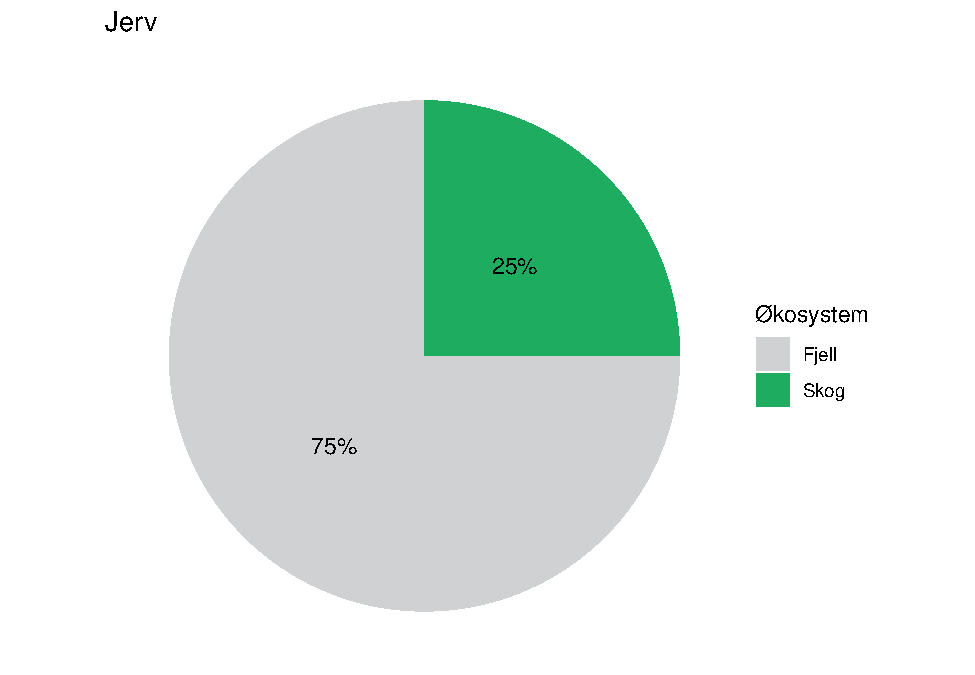
\includegraphics{04-other_figures_files/figure-latex/unnamed-chunk-10-2.pdf} 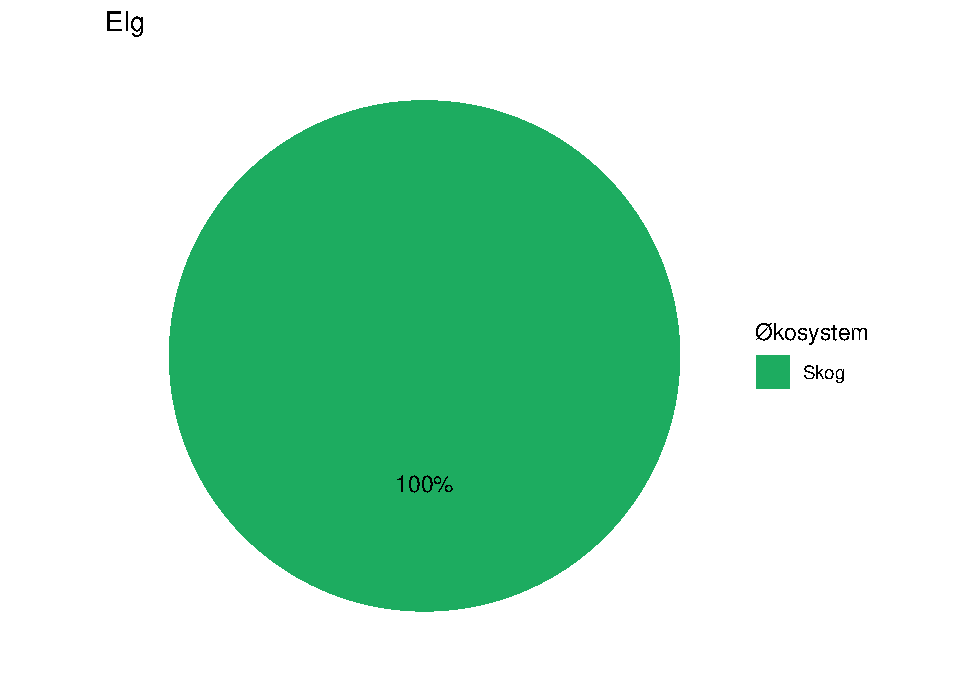
\includegraphics{04-other_figures_files/figure-latex/unnamed-chunk-10-3.pdf} 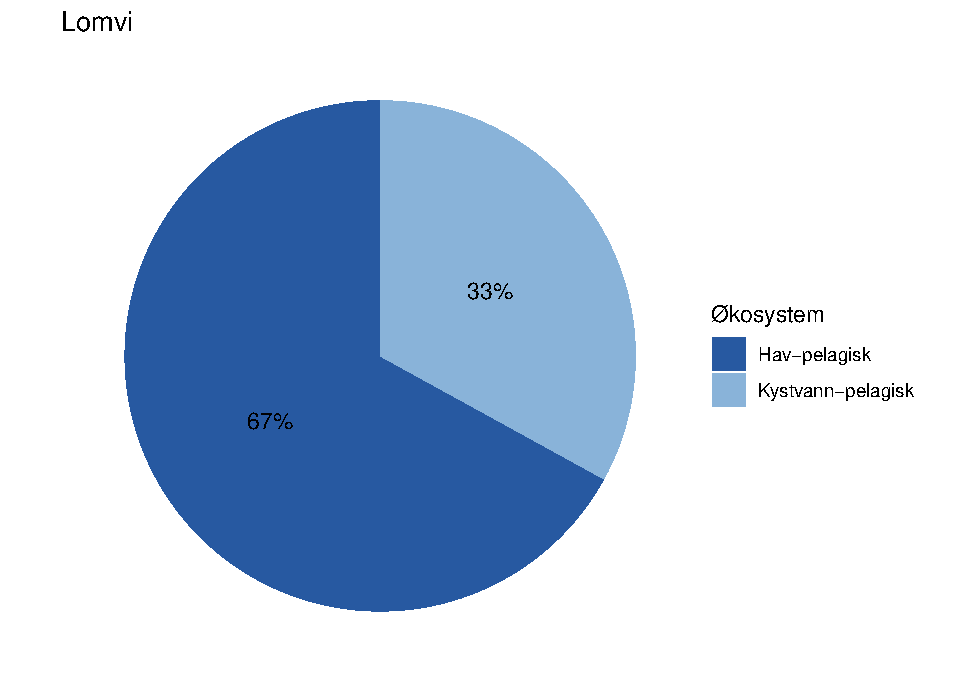
\includegraphics{04-other_figures_files/figure-latex/unnamed-chunk-10-4.pdf} 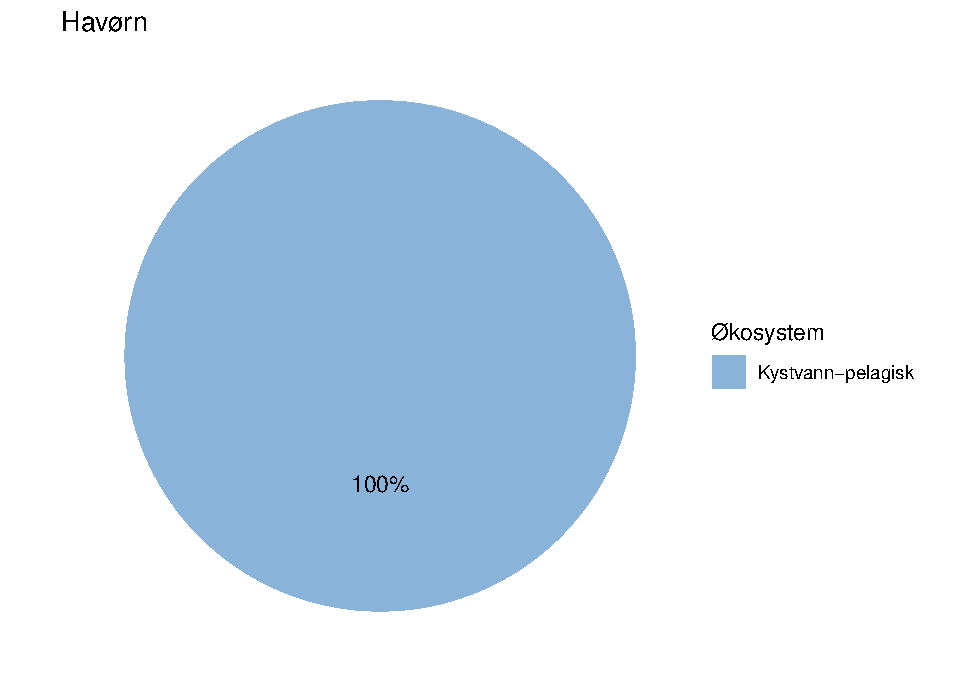
\includegraphics{04-other_figures_files/figure-latex/unnamed-chunk-10-5.pdf} 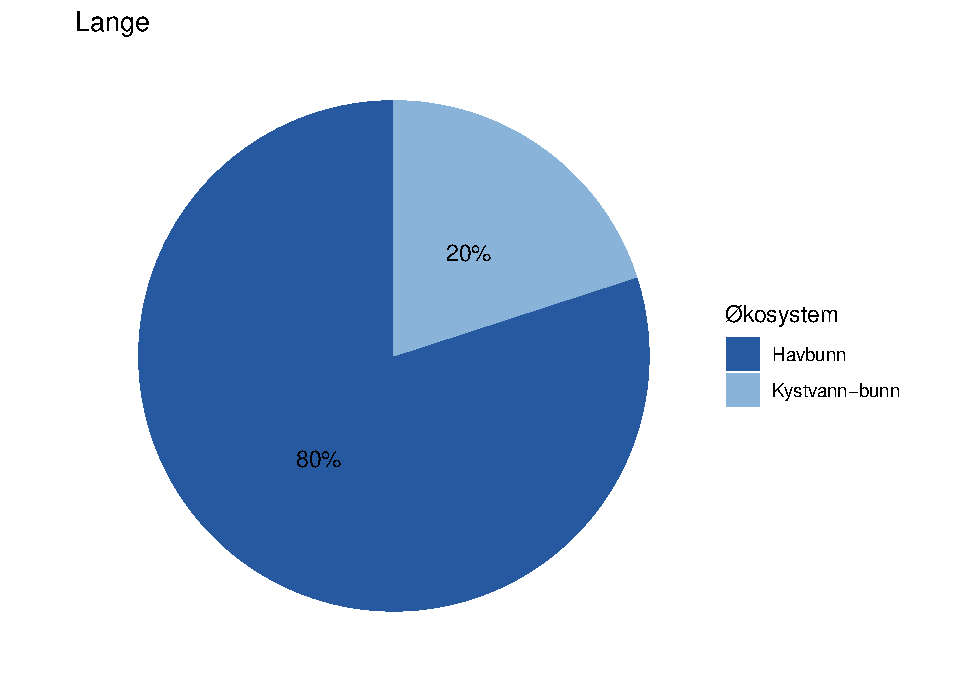
\includegraphics{04-other_figures_files/figure-latex/unnamed-chunk-10-6.pdf}
Depending on how large these pie charts should appear on the website in the end, it may be necessary to move the percentage labels outside the pies. Doing that is a bit more cumbersome, but works with the code below unless the indicator belongs 100 \% to one dataset. When that is the case, the solution below does not print the percentage label at all (see indicator Lange) and I have not figured out how to fix that yet.

\begin{Shaded}
\begin{Highlighting}[]
\ControlFlowTok{for}\NormalTok{(i }\ControlFlowTok{in} \DecValTok{1}\SpecialCharTok{:}\FunctionTok{length}\NormalTok{(indicator))\{}
  
\NormalTok{  sub\_fidData }\OtherTok{\textless{}{-}}\NormalTok{ fidData[}\FunctionTok{which}\NormalTok{(fidData}\SpecialCharTok{$}\NormalTok{indicator }\SpecialCharTok{==}\NormalTok{ indicator[i]),]}
  
\NormalTok{  posData }\OtherTok{\textless{}{-}}\NormalTok{ sub\_fidData }\SpecialCharTok{\%\textgreater{}\%} 
  \FunctionTok{mutate}\NormalTok{(}\AttributeTok{csum =} \FunctionTok{rev}\NormalTok{(}\FunctionTok{cumsum}\NormalTok{(}\FunctionTok{rev}\NormalTok{(fidelity))), }
         \AttributeTok{pos =}\NormalTok{ fidelity}\SpecialCharTok{/}\DecValTok{2} \SpecialCharTok{+} \FunctionTok{lead}\NormalTok{(csum, }\DecValTok{1}\NormalTok{),}
         \AttributeTok{pos =} \FunctionTok{if\_else}\NormalTok{(}\FunctionTok{is.na}\NormalTok{(pos), fidelity}\SpecialCharTok{/}\DecValTok{2}\NormalTok{, pos))}
  
  \FunctionTok{print}\NormalTok{(}
  \FunctionTok{ggplot}\NormalTok{(sub\_fidData, }\FunctionTok{aes}\NormalTok{(}\AttributeTok{x =} \StringTok{""}\NormalTok{, }\AttributeTok{y =}\NormalTok{ fidelity, }\AttributeTok{fill =}\NormalTok{ ecosystem)) }\SpecialCharTok{+}
    \FunctionTok{ggtitle}\NormalTok{(indicator[i]) }\SpecialCharTok{+} 
    \FunctionTok{geom\_bar}\NormalTok{(}\AttributeTok{stat =} \StringTok{"identity"}\NormalTok{) }\SpecialCharTok{+}
    \FunctionTok{coord\_polar}\NormalTok{(}\AttributeTok{theta =} \StringTok{"y"}\NormalTok{) }\SpecialCharTok{+}
    \CommentTok{\#scale\_fill\_manual(values = EcoSys\_cols) + }
    \FunctionTok{scale\_fill\_manual}\NormalTok{(}\AttributeTok{name =} \StringTok{"Økosystem"}\NormalTok{, }\AttributeTok{values =}\NormalTok{ EcoSys\_cols[}\FunctionTok{which}\NormalTok{(}\FunctionTok{names}\NormalTok{(EcoSys\_cols) }\SpecialCharTok{\%in\%}\NormalTok{ sub\_fidData}\SpecialCharTok{$}\NormalTok{ecosystem)]) }\SpecialCharTok{+} 
    \FunctionTok{scale\_y\_continuous}\NormalTok{(}\AttributeTok{breaks =}\NormalTok{ posData}\SpecialCharTok{$}\NormalTok{pos, }\AttributeTok{labels =} \FunctionTok{paste0}\NormalTok{(sub\_fidData}\SpecialCharTok{$}\NormalTok{fidelity, }\StringTok{"\%"}\NormalTok{)) }\SpecialCharTok{+}
    \FunctionTok{theme}\NormalTok{(}\AttributeTok{axis.ticks =} \FunctionTok{element\_blank}\NormalTok{(),}
          \AttributeTok{axis.title =} \FunctionTok{element\_blank}\NormalTok{(),}
          \AttributeTok{axis.text =} \FunctionTok{element\_text}\NormalTok{(}\AttributeTok{size =} \DecValTok{15}\NormalTok{), }
          \AttributeTok{panel.background =} \FunctionTok{element\_rect}\NormalTok{(}\AttributeTok{fill =} \StringTok{"white"}\NormalTok{))}
\NormalTok{  )}

\NormalTok{\}}
\end{Highlighting}
\end{Shaded}

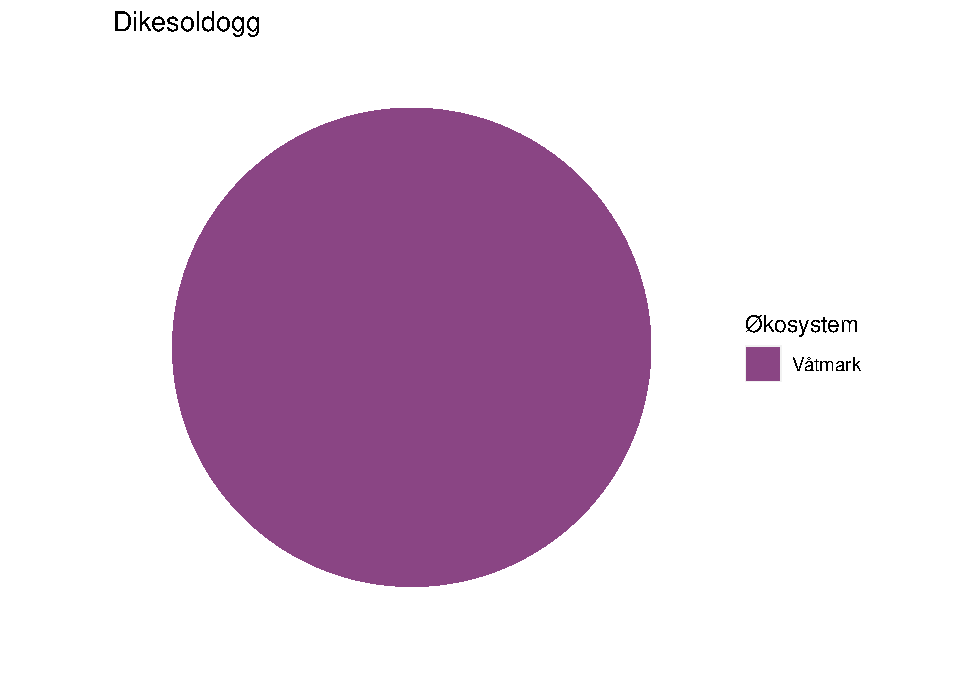
\includegraphics{04-other_figures_files/figure-latex/unnamed-chunk-11-1.pdf} 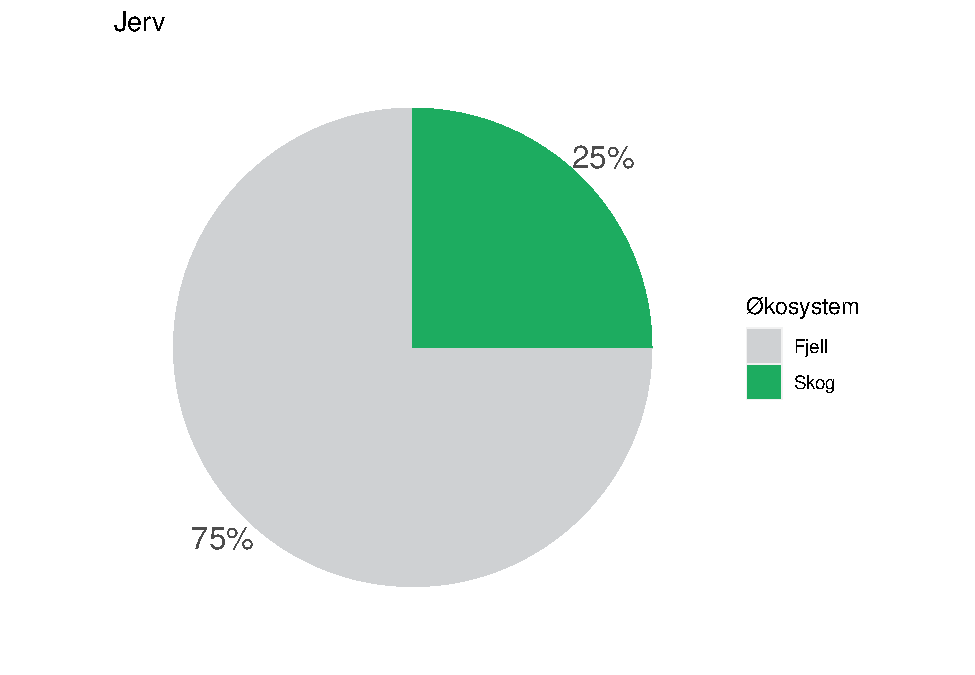
\includegraphics{04-other_figures_files/figure-latex/unnamed-chunk-11-2.pdf} 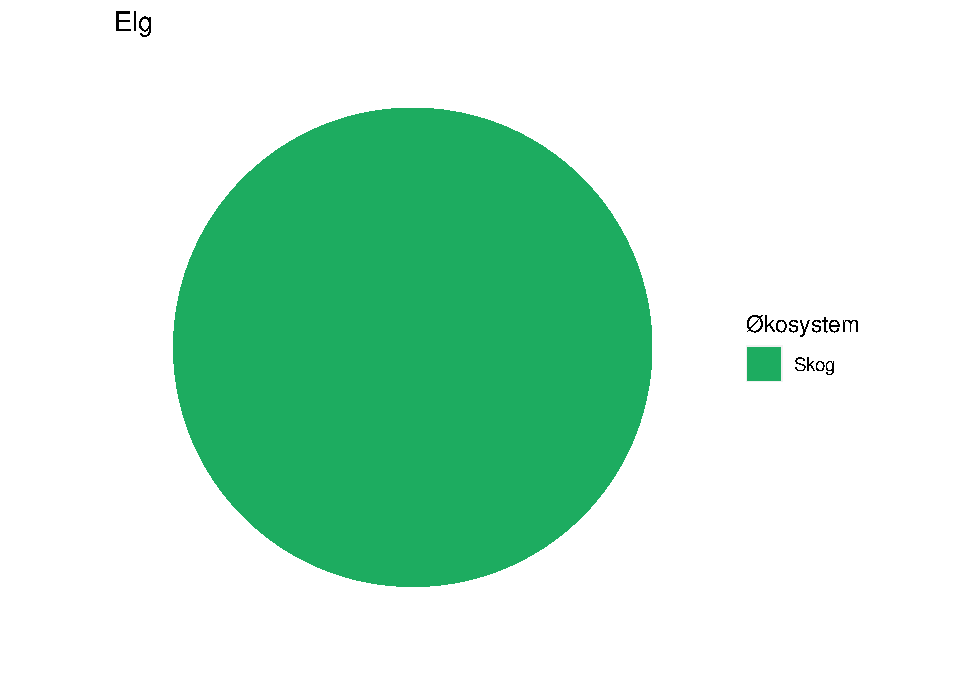
\includegraphics{04-other_figures_files/figure-latex/unnamed-chunk-11-3.pdf} 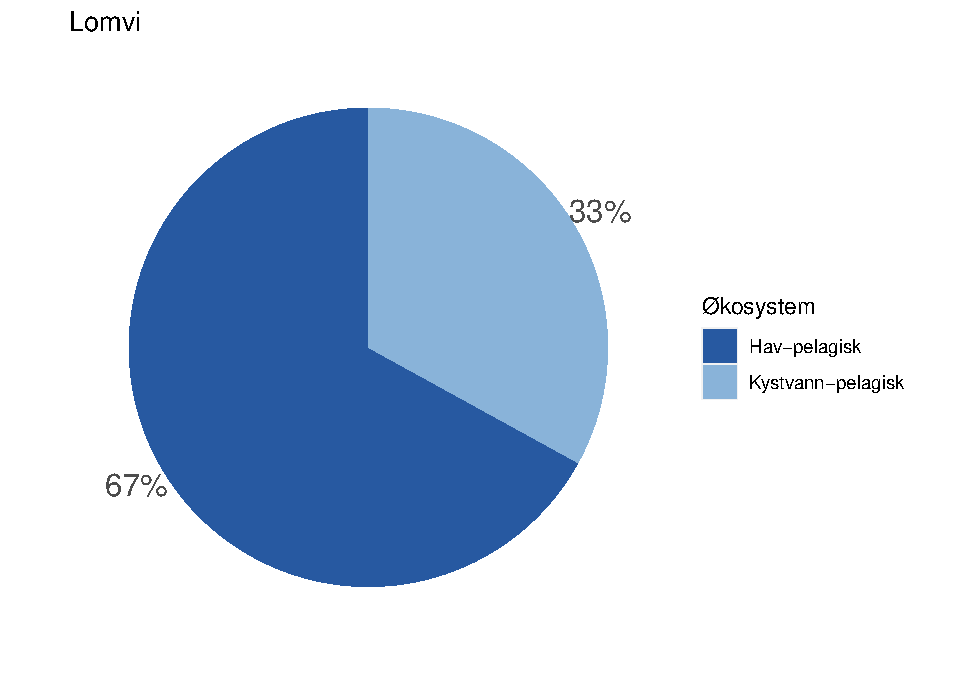
\includegraphics{04-other_figures_files/figure-latex/unnamed-chunk-11-4.pdf} 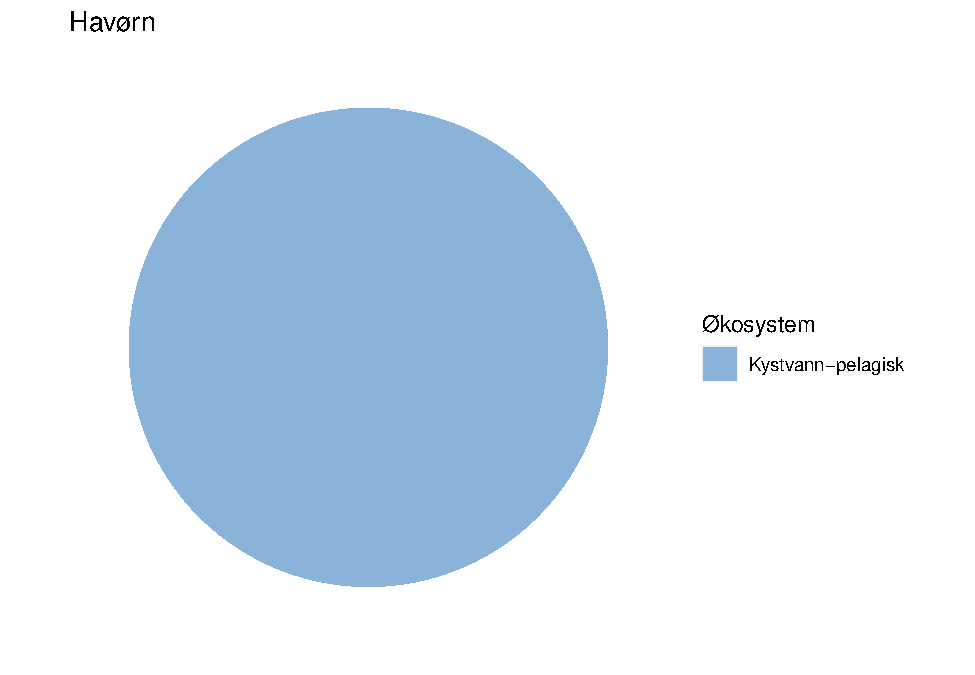
\includegraphics{04-other_figures_files/figure-latex/unnamed-chunk-11-5.pdf} 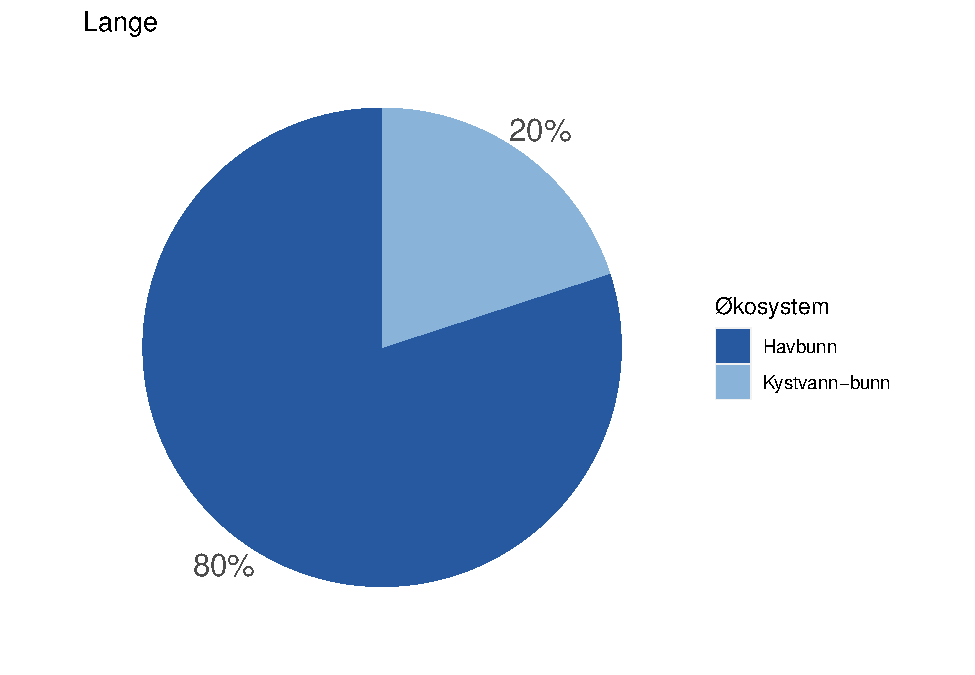
\includegraphics{04-other_figures_files/figure-latex/unnamed-chunk-11-6.pdf}

\hypertarget{impact-factor-wordclouds}{%
\section{Impact factor wordclouds}\label{impact-factor-wordclouds}}

\begin{Shaded}
\begin{Highlighting}[]

\FunctionTok{library}\NormalTok{(wordcloud)}
\FunctionTok{library}\NormalTok{(NIcalc)}
\FunctionTok{library}\NormalTok{(wordcloud2)}
\FunctionTok{library}\NormalTok{(RColorBrewer)}
\FunctionTok{library}\NormalTok{(readxl)}
\FunctionTok{library}\NormalTok{(dplyr)}
\FunctionTok{library}\NormalTok{(tm)}
\end{Highlighting}
\end{Shaded}

As per now, the website shows the most important impact factors for each indicator as a list in a pop-up window on the top-right. This is information that is likely of great interest to the general public, and would benefit from being placed more visible on the website and in a more engaging way than as a list. One attractive alternative way of presenting is via wordclouds.

The following wordcloud figures show the pressure factors for each indicator, where both the color saturation and text size represent the importance of each pressure factor. Small text size and low saturation means low importance, while large text size represent pressure factors with high importance to the indicator.

\begin{Shaded}
\begin{Highlighting}[]

\CommentTok{\# Load dataset}
\NormalTok{pressure }\OtherTok{=} \FunctionTok{read\_excel}\NormalTok{(}\StringTok{"P:/41201612\_naturindeks\_2021\_2023\_database\_og\_innsynslosning/Pilot\_Forbedring\_Innsynsløsning/R/Indikator\_paavirkning.xlsx"}\NormalTok{)}

\CommentTok{\# Filter for species of interest}
\NormalTok{pressure }\OtherTok{=}\NormalTok{ pressure }\SpecialCharTok{\%\textgreater{}\%} \FunctionTok{filter}\NormalTok{(navn\_norsk }\SpecialCharTok{==} \StringTok{"Elg"} \SpecialCharTok{|}\NormalTok{ navn\_norsk }\SpecialCharTok{==} \StringTok{"Dikesoldogg"} \SpecialCharTok{|}\NormalTok{ navn\_norsk }\SpecialCharTok{==} \StringTok{"Havørn"} \SpecialCharTok{|}\NormalTok{ navn\_norsk }\SpecialCharTok{==} \StringTok{"Lange"} \SpecialCharTok{|}\NormalTok{ navn\_norsk }\SpecialCharTok{==} \StringTok{"Jerv"} \SpecialCharTok{|}\NormalTok{ navn\_norsk }\SpecialCharTok{==} \StringTok{"Lomvi"}\NormalTok{) }\CommentTok{\# NB {-} Jerv was not included in the provided excel file}
\NormalTok{pressure }\OtherTok{=} \FunctionTok{arrange}\NormalTok{(pressure, }\AttributeTok{by =}\NormalTok{ navn\_norsk)}
\NormalTok{pressure }\OtherTok{=}\NormalTok{ pressure }\SpecialCharTok{\%\textgreater{}\%} \FunctionTok{rename}\NormalTok{(}\AttributeTok{PressureFactor =}\NormalTok{ Paavirkningsfaktor, }\AttributeTok{PressureValue =}\NormalTok{ FK\_PaavirkningsverdiID)}

\CommentTok{\# Remove all instances of "Ikke rel/ukjent" category" and increase the value of pressure factors for better contrast in wordcloud figures}
\NormalTok{pressure }\OtherTok{=}\NormalTok{ pressure }\SpecialCharTok{\%\textgreater{}\%} \FunctionTok{filter}\NormalTok{(PressureValue }\SpecialCharTok{!=} \DecValTok{7}\NormalTok{) }\SpecialCharTok{\%\textgreater{}\%} \FunctionTok{mutate}\NormalTok{(}\AttributeTok{PressureValue =}\NormalTok{ PressureValue}\SpecialCharTok{*}\DecValTok{2}\NormalTok{) }

\CommentTok{\# Create separate datasets for the different species}
\NormalTok{dikesoldogg }\OtherTok{=}\NormalTok{ pressure }\SpecialCharTok{\%\textgreater{}\%} \FunctionTok{filter}\NormalTok{(navn\_norsk }\SpecialCharTok{==} \StringTok{"Dikesoldogg"}\NormalTok{) }\SpecialCharTok{\%\textgreater{}\%}\NormalTok{ dplyr}\SpecialCharTok{::}\FunctionTok{select}\NormalTok{(PressureFactor, PressureValue)}

\NormalTok{elg }\OtherTok{=}\NormalTok{ pressure }\SpecialCharTok{\%\textgreater{}\%} \FunctionTok{filter}\NormalTok{(navn\_norsk }\SpecialCharTok{==} \StringTok{"Elg"}\NormalTok{) }\SpecialCharTok{\%\textgreater{}\%}\NormalTok{ dplyr}\SpecialCharTok{::}\FunctionTok{select}\NormalTok{(PressureFactor, PressureValue)}

\NormalTok{havørn }\OtherTok{=}\NormalTok{ pressure }\SpecialCharTok{\%\textgreater{}\%} \FunctionTok{filter}\NormalTok{(navn\_norsk }\SpecialCharTok{==} \StringTok{"Havørn"}\NormalTok{) }\SpecialCharTok{\%\textgreater{}\%}\NormalTok{ dplyr}\SpecialCharTok{::}\FunctionTok{select}\NormalTok{(PressureFactor, PressureValue)}

\NormalTok{lange }\OtherTok{=}\NormalTok{ pressure }\SpecialCharTok{\%\textgreater{}\%} \FunctionTok{filter}\NormalTok{(navn\_norsk }\SpecialCharTok{==} \StringTok{"Lange"}\NormalTok{) }\SpecialCharTok{\%\textgreater{}\%}\NormalTok{ dplyr}\SpecialCharTok{::}\FunctionTok{select}\NormalTok{(PressureFactor, PressureValue)}

\NormalTok{lomvi }\OtherTok{=}\NormalTok{ pressure }\SpecialCharTok{\%\textgreater{}\%} \FunctionTok{filter}\NormalTok{(navn\_norsk }\SpecialCharTok{==} \StringTok{"Lomvi"}\NormalTok{) }\SpecialCharTok{\%\textgreater{}\%}\NormalTok{ dplyr}\SpecialCharTok{::}\FunctionTok{select}\NormalTok{(PressureFactor, PressureValue)}

\CommentTok{\# Create a custom color gradient (green in this case)}
\NormalTok{pressureColors }\OtherTok{=} \FunctionTok{c}\NormalTok{(}\StringTok{"\#bde4aa"}\NormalTok{, }\StringTok{"\#addb9d"}\NormalTok{, }\StringTok{"\#9cd28f"}\NormalTok{, }\StringTok{"\#8cc982"}\NormalTok{, }\StringTok{"\#7dc275"}\NormalTok{, }\StringTok{"\#6cb967"}\NormalTok{, }\StringTok{"\#5db15a"}\NormalTok{, }\StringTok{"\#50a54e"}\NormalTok{, }\StringTok{"\#479845"}\NormalTok{, }\StringTok{"\#3f8c3b"}\NormalTok{, }\StringTok{"\#367e31"}\NormalTok{, }\StringTok{"\#2e7228"}\NormalTok{, }\StringTok{"\#25661f"}\NormalTok{) }
\end{Highlighting}
\end{Shaded}

\hypertarget{dikesoldogg-oblong-leaved-sundew}{%
\subsection{Dikesoldogg (oblong-leaved sundew)}\label{dikesoldogg-oblong-leaved-sundew}}

\begin{Shaded}
\begin{Highlighting}[]

\CommentTok{\# Dikesoldogg}
\FunctionTok{wordcloud}\NormalTok{(}\AttributeTok{words =}\NormalTok{ dikesoldogg}\SpecialCharTok{$}\NormalTok{PressureFactor, }\AttributeTok{freq =}\NormalTok{ dikesoldogg}\SpecialCharTok{$}\NormalTok{PressureValue, }\AttributeTok{min.freq =} \DecValTok{1}\NormalTok{, }\AttributeTok{max.words =} \DecValTok{200}\NormalTok{, }\AttributeTok{random.order =} \ConstantTok{FALSE}\NormalTok{, }\AttributeTok{rot.per =} \FloatTok{0.35}\NormalTok{, }\AttributeTok{colors =}\NormalTok{ pressureColors, }\AttributeTok{scale =} \FunctionTok{c}\NormalTok{(}\FloatTok{1.5}\NormalTok{, }\FloatTok{0.5}\NormalTok{)) }\CommentTok{\# use rot.per to set the percentage of words that are at a 90 degree angle}
\end{Highlighting}
\end{Shaded}


\includegraphics{04-other_figures_files/figure-latex/Wordcloud - Dikesoldogg-1.pdf}

\hypertarget{elg-moose}{%
\subsection{Elg (Moose)}\label{elg-moose}}

\begin{Shaded}
\begin{Highlighting}[]

\FunctionTok{wordcloud}\NormalTok{(}\AttributeTok{words =}\NormalTok{ elg}\SpecialCharTok{$}\NormalTok{PressureFactor, }\AttributeTok{freq =}\NormalTok{ elg}\SpecialCharTok{$}\NormalTok{PressureValue, }\AttributeTok{min.freq =} \DecValTok{1}\NormalTok{, }\AttributeTok{max.words =} \DecValTok{200}\NormalTok{, }\AttributeTok{random.order =} \ConstantTok{FALSE}\NormalTok{, }\AttributeTok{rot.per =} \FloatTok{0.35}\NormalTok{, }\AttributeTok{colors =}\NormalTok{ pressureColors, }\AttributeTok{scale =} \FunctionTok{c}\NormalTok{(}\FloatTok{1.5}\NormalTok{, }\FloatTok{0.5}\NormalTok{))}
\end{Highlighting}
\end{Shaded}

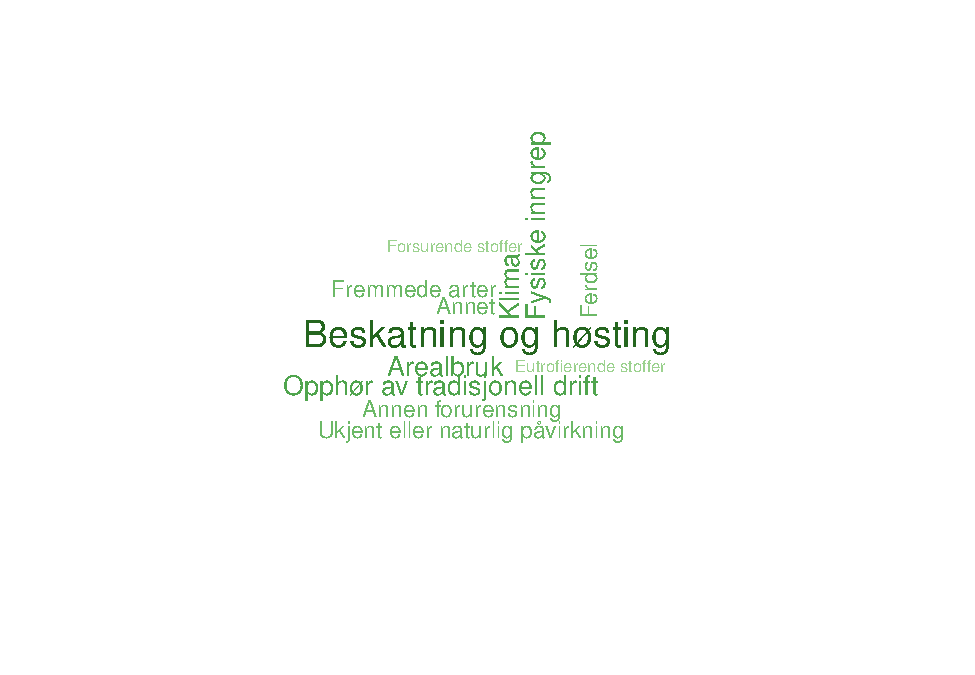
\includegraphics{04-other_figures_files/figure-latex/Wordcloud - Elg-1.pdf}

\hypertarget{havuxf8rn-white-tailed-eagle}{%
\subsection{Havørn (White-tailed eagle)}\label{havuxf8rn-white-tailed-eagle}}

\begin{Shaded}
\begin{Highlighting}[]

\FunctionTok{wordcloud}\NormalTok{(}\AttributeTok{words =}\NormalTok{ havørn}\SpecialCharTok{$}\NormalTok{PressureFactor, }\AttributeTok{freq =}\NormalTok{ havørn}\SpecialCharTok{$}\NormalTok{PressureValue, }\AttributeTok{min.freq =} \DecValTok{1}\NormalTok{, }\AttributeTok{max.words =} \DecValTok{200}\NormalTok{, }\AttributeTok{random.order =} \ConstantTok{FALSE}\NormalTok{, }\AttributeTok{rot.per =} \FloatTok{0.35}\NormalTok{, }\AttributeTok{colors =}\NormalTok{ pressureColors, }\AttributeTok{scale =} \FunctionTok{c}\NormalTok{(}\FloatTok{1.5}\NormalTok{, }\FloatTok{0.5}\NormalTok{))}
\end{Highlighting}
\end{Shaded}

\includegraphics{04-other_figures_files/figure-latex/Wordcloud - Havørn-1.pdf}

\hypertarget{lange-common-ling}{%
\subsection{Lange (Common ling)}\label{lange-common-ling}}

\begin{Shaded}
\begin{Highlighting}[]

\FunctionTok{wordcloud}\NormalTok{(}\AttributeTok{words =}\NormalTok{ lange}\SpecialCharTok{$}\NormalTok{PressureFactor, }\AttributeTok{freq =}\NormalTok{ lange}\SpecialCharTok{$}\NormalTok{PressureValue, }\AttributeTok{min.freq =} \DecValTok{1}\NormalTok{, }\AttributeTok{max.words =} \DecValTok{200}\NormalTok{, }\AttributeTok{random.order =} \ConstantTok{FALSE}\NormalTok{, }\AttributeTok{rot.per =} \FloatTok{0.35}\NormalTok{, }\AttributeTok{colors =}\NormalTok{ pressureColors, }\AttributeTok{scale =} \FunctionTok{c}\NormalTok{(}\FloatTok{1.5}\NormalTok{, }\FloatTok{0.5}\NormalTok{))}
\end{Highlighting}
\end{Shaded}

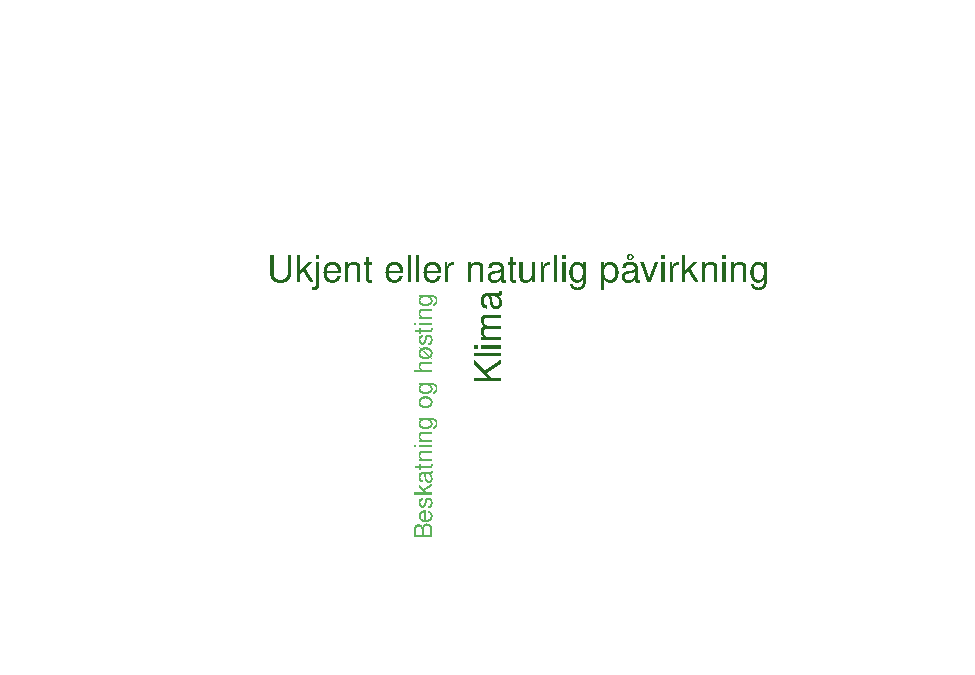
\includegraphics{04-other_figures_files/figure-latex/Wordcloud - Lange-1.pdf}

\hypertarget{lomvi-common-guillemot}{%
\subsection{Lomvi (common guillemot)}\label{lomvi-common-guillemot}}

\begin{Shaded}
\begin{Highlighting}[]

\FunctionTok{wordcloud}\NormalTok{(}\AttributeTok{words =}\NormalTok{ lomvi}\SpecialCharTok{$}\NormalTok{PressureFactor, }\AttributeTok{freq =}\NormalTok{ lomvi}\SpecialCharTok{$}\NormalTok{PressureValue, }\AttributeTok{min.freq =} \DecValTok{1}\NormalTok{, }\AttributeTok{max.words =} \DecValTok{200}\NormalTok{, }\AttributeTok{random.order =} \ConstantTok{FALSE}\NormalTok{, }\AttributeTok{rot.per =} \FloatTok{0.35}\NormalTok{, }\AttributeTok{colors =}\NormalTok{ pressureColors, }\AttributeTok{scale =} \FunctionTok{c}\NormalTok{(}\FloatTok{1.5}\NormalTok{, }\FloatTok{0.5}\NormalTok{))}
\end{Highlighting}
\end{Shaded}

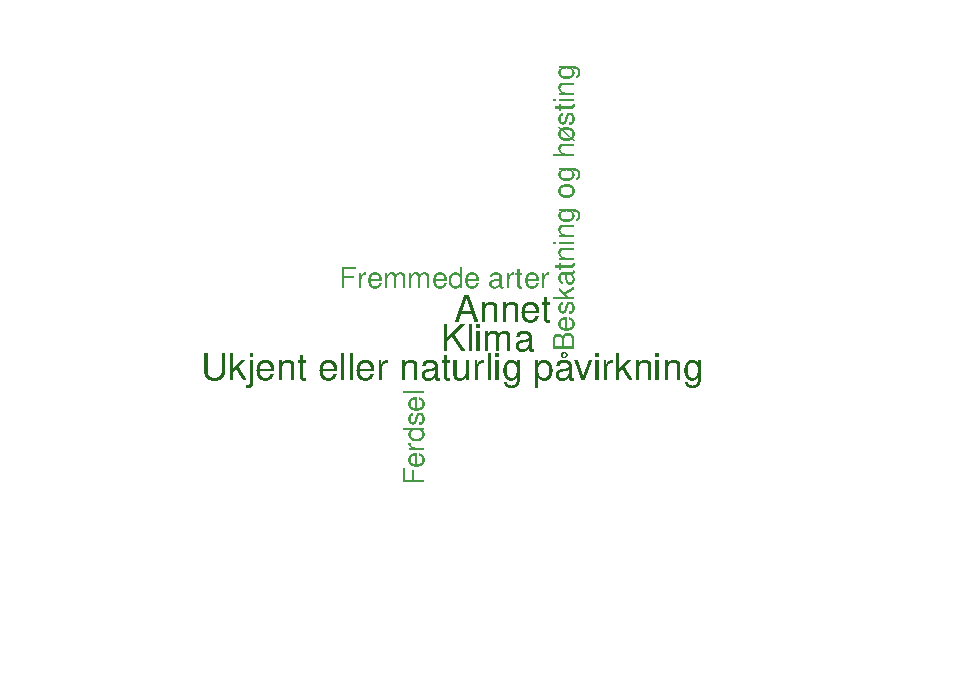
\includegraphics{04-other_figures_files/figure-latex/Wordcloud - Lomvi-1.pdf}

\hypertarget{data-type}{%
\section{Data type}\label{data-type}}

\begin{Shaded}
\begin{Highlighting}[]
\FunctionTok{source}\NormalTok{(}\StringTok{"R/colorPalettes.R"}\NormalTok{)}
\end{Highlighting}
\end{Shaded}

\begin{Shaded}
\begin{Highlighting}[]
\CommentTok{\#Elg datatyper}
\NormalTok{data }\OtherTok{\textless{}{-}} \FunctionTok{data.frame}\NormalTok{(}
  \AttributeTok{category=}\FunctionTok{c}\NormalTok{(}\StringTok{"Ekspert"}\NormalTok{, }
             \StringTok{"Modeller"}\NormalTok{, }
             \StringTok{"Overvåkning"}\NormalTok{),}
  \AttributeTok{count=}\FunctionTok{c}\NormalTok{(}\FloatTok{4.9}\NormalTok{, }\FloatTok{95.1}\NormalTok{, }\DecValTok{0}\NormalTok{)}
\NormalTok{)}

\CommentTok{\# load library}
\FunctionTok{library}\NormalTok{(tidyverse)}
\CommentTok{\# Compute percentages}
\NormalTok{data}\SpecialCharTok{$}\NormalTok{fraction }\OtherTok{\textless{}{-}}\NormalTok{ data}\SpecialCharTok{$}\NormalTok{count }\SpecialCharTok{/} \FunctionTok{sum}\NormalTok{(data}\SpecialCharTok{$}\NormalTok{count)}

\CommentTok{\# Compute the cumulative percentages (top of each rectangle)}
\NormalTok{data}\SpecialCharTok{$}\NormalTok{ymax }\OtherTok{\textless{}{-}} \FunctionTok{cumsum}\NormalTok{(data}\SpecialCharTok{$}\NormalTok{fraction)}

\CommentTok{\# Compute the bottom of each rectangle}
\NormalTok{data}\SpecialCharTok{$}\NormalTok{ymin }\OtherTok{\textless{}{-}} \FunctionTok{c}\NormalTok{(}\DecValTok{0}\NormalTok{, }\FunctionTok{head}\NormalTok{(data}\SpecialCharTok{$}\NormalTok{ymax, }\AttributeTok{n=}\SpecialCharTok{{-}}\DecValTok{1}\NormalTok{))}

\CommentTok{\# Compute label position}
\NormalTok{data}\SpecialCharTok{$}\NormalTok{labelPosition }\OtherTok{\textless{}{-}}\NormalTok{ (data}\SpecialCharTok{$}\NormalTok{ymax }\SpecialCharTok{+}\NormalTok{ data}\SpecialCharTok{$}\NormalTok{ymin) }\SpecialCharTok{/} \DecValTok{2}
\NormalTok{data}\SpecialCharTok{$}\NormalTok{labelPosition[}\DecValTok{3}\NormalTok{]}\OtherTok{\textless{}{-}}\FloatTok{0.8}
\CommentTok{\# Compute a good label}
\NormalTok{data}\SpecialCharTok{$}\NormalTok{label }\OtherTok{\textless{}{-}} \FunctionTok{paste0}\NormalTok{(data}\SpecialCharTok{$}\NormalTok{category, }\StringTok{"}\SpecialCharTok{\textbackslash{}n}\StringTok{ "}\NormalTok{, data}\SpecialCharTok{$}\NormalTok{count, }\StringTok{" \%"}\NormalTok{)}
\FunctionTok{library}\NormalTok{(ggrepel)}
\CommentTok{\#\textgreater{} Warning: package \textquotesingle{}ggrepel\textquotesingle{} was built under R version 4.1.3}
\CommentTok{\# Make the plot}
\FunctionTok{ggplot}\NormalTok{(data, }\FunctionTok{aes}\NormalTok{(}\AttributeTok{ymax=}\NormalTok{ymax, }\AttributeTok{ymin=}\NormalTok{ymin, }\AttributeTok{xmax=}\DecValTok{4}\NormalTok{, }\AttributeTok{xmin=}\DecValTok{3}\NormalTok{, }\AttributeTok{fill=}\NormalTok{category)) }\SpecialCharTok{+}
  \FunctionTok{geom\_rect}\NormalTok{() }\SpecialCharTok{+}
  \FunctionTok{geom\_text}\NormalTok{(}\AttributeTok{x=}\DecValTok{2}\NormalTok{, }\FunctionTok{aes}\NormalTok{(}\AttributeTok{y=}\NormalTok{labelPosition, }\AttributeTok{label=}\NormalTok{label, }\AttributeTok{color=}\NormalTok{category), }\AttributeTok{size=}\FloatTok{2.5}\NormalTok{) }\SpecialCharTok{+} \CommentTok{\# x here controls label position (inner / outer)}
  \FunctionTok{scale\_fill\_NIviz\_d}\NormalTok{(}\StringTok{"IndMap\_cols"}\NormalTok{) }\SpecialCharTok{+}
  \FunctionTok{scale\_colour\_NIviz\_d}\NormalTok{(}\StringTok{"IndMap\_cols"}\NormalTok{) }\SpecialCharTok{+}
  \FunctionTok{coord\_polar}\NormalTok{(}\AttributeTok{theta=}\StringTok{"y"}\NormalTok{) }\SpecialCharTok{+}
  \FunctionTok{xlim}\NormalTok{(}\FunctionTok{c}\NormalTok{(}\SpecialCharTok{{-}}\DecValTok{1}\NormalTok{, }\DecValTok{4}\NormalTok{)) }\SpecialCharTok{+}
  \FunctionTok{theme\_void}\NormalTok{() }\SpecialCharTok{+}
  \FunctionTok{theme}\NormalTok{(}\AttributeTok{legend.position =} \StringTok{"none"}\NormalTok{)}
\end{Highlighting}
\end{Shaded}

\includegraphics{04-other_figures_files/figure-latex/unnamed-chunk-13-1.pdf}

  \bibliography{book.bib,packages.bib}

\end{document}
